% +--------------------------------------------------------------------+
% | Chapter 03 - Characterization of (h,e)-implications				   |
% +--------------------------------------------------------------------+

\graphicspath{{./_figures/03_heimplications/}}

\section{Introduction}\label{section:introduction(h,e))}

In this chapter, we are interested in the study of the family of generalized $(h,e)$-implications. These fuzzy implication functions were defined for the first time in \cite{Massanet2011A} under the motivation of generalizing $h$-implications to a new family of functions satisfying the property \NPe, that is, $I(e,y)=y$ for all $y \in [0,1]$ and some $e \in (0,1)$.  The family of generalized $(h,e)$-implications has presented very interesting properties such as the controlled increasingness in the second variable by the parameter $e$ or that they constitute a whole family of fuzzy implication functions fulfilling the exchange principle but not the law of importation for any t-norm $T$ \cite{Massanet2011B}. Additionally, they have been applied on image processing for edge detection (see \cite{Gonzalez-Hidalgo2015}), obtaining good results with respect to other families of fuzzy implication functions. Although the properties of $(h,e)$-implications were analyzed for the first time in \cite{Massanet2011A}, in \cite{Hlinena2013} it was pointed out that a more general definition was possible. Therefore, our first contribution is to adapt all the existing results to this more general definition and to provide all the proofs. 

In \cite{Massanet2012A} it was proved that $h$-implications were characterized by the fact that their structure is determined by two Yager's implications through the threshold horizontal method \cite{Massanet2012A}. More specifically, the structure of an $h$-implication is like an adequately scaled $f$-generated implication whenever $y \leq e$ and like an adequately scaled $g$-generated implication whenever $y>e$. In this chapter, as a second contribution, we provide a similar result for $(h,e)$-implications but, in our case,  the structure of $(h,e)$-implications is described in terms of two subfamilies of some new families of fuzzy implication functions which are generalizations of Yager's implications, called $(f,g)$ and $(g,f)$-implications \cite{Massanet2013B}. Until nowadays there has been several proposals of generalizations of Yager's implications by considering different approaches: generalizing the inner factors $x$ and  $\frac{1}{x}$, in the expression of $f$ and $g$-generated implications, respectively \cite{Massanet2013B,VemuriJayaram2012,XieLiu2013,PeiZhu2017}, considering a different internal function from the product \cite{Hlinena2012,Massanet2012C,ZhangLiu2013}; among others \cite{Liu2012,ZhangZhang2017}. The families of $(f,g)$ and $(g,f)$-implications are of the first kind since they consider the internal factor $x$ as a continuous and strictly increasing function $g:[0,1] \to [0,+\infty]$ with $g(0)=0$ and $\frac{1}{x}$ as a continuous and strictly decreasing function $f:[0,1] \to [0,+\infty]$ with $f(0)=+\infty$. This approach is different from all the other generalization proposals, and then the interest in these two families is twofold: to describe the structure of generalized $(h,e)$-implications and to study these families in order to compare their properties with other generalizations considered in the literature. Although these two families were preliminary studied in \cite{Massanet2013B}, the results were provided without any proof and some of them were partially erroneous. Our third contribution is to provide the proofs of all the results and to rectify the mistakes in some statements.

Next, we solve the problem of the characterization of generalized $(h,e)$-implications. To do so, we first provide the characterizations of two subfamilies of $(f,g)$ and $(g,f)$-implications, called $(f,e)$ and $(g,e)$-implications. Consequently, using the representation theorem of generalized $(h,e)$-implications, we provide an axiomatic characterization of this family in terms of their own properties. These three characterizations are based on two novel properties of fuzzy implication functions which are variations of the law of importation different from the generalizations found in the literature \cite{Baczynski2020,Massanet2011B}. In addition, we perform a similar study like the one presented in \cite{Vemuri2014} to provide a representation theorem for $(f,e)$ and $(g,e)$-implications. 

The chapter is structured as follows:  in Section \ref{section:generalized(h,e)impl} the family of generalized $(h,e)$-implications and its main properties are recalled and a proof of the representation theorem is given; in Section \ref{section:(f,g)&(g,f)} the families of $(f,g)$ and $(g,f)$-implications are presented and their properties are studied; in Section \ref{section:characterizations(f,e)&(g,e)} the characterizations of $(f,e)$ and $(g,e)$-implications are presented and in Section \ref{section:representation(f,e)} the representation theorem for $(f,e)$ and $(g,e)$-implications is obtained; in Section \ref{section:characterization(h,e)} the characterization of generalized $(h,e)$-implications is given. The chapter ends in Section \ref{section:conclusionshe} with some conclusions and future work.

\section{Definition and additional properties of generalized $(h,e)$-implications}\label{section:generalized(h,e)impl}

In \cite{Massanet2011A} a new class of fuzzy implication functions was presented, the family of $(h,e)$-implications. The motivation behind its definition was modifying the $h$-implications towards fulfilling the property \NPe. Indeed, the family of $h$-implications presented an unexpected behavior. Most of the families of fuzzy implication functions generated from uninorms such as RU-implications \cite{DeBaets1999}, which are generalizations of R-implications, tend to satisfy \NPe instead of \NP. Being $h$-generators the additive generators of representable uninorms, it would be expected that this family of fuzzy implications functions would satisfy \NPe instead of \NP. This is achieved with a slight modification in the definition leading to the so-called $(h,e)$-implications. 

Although $(h,e)$-implications were first defined in \cite[Definition 7]{Massanet2011A}, in \cite{Hlinena2013} it was pointed out that a more general definition allowing $h(0)>-\infty$ was possible. The latter is the one recalled here.

\begin{definition}[\textbf{\cite[Definition 11]{Hlinena2013}}] Fix an $e \in (0,1)$ and let $h:[0,1] \to [-\infty,+\infty]$ be a strictly increasing and continuous function with $h(e)=0$ and $h(1)= +\infty$. The function $I^{h_g,e}:[0,1]^2 \to [0,1]$ defined by
	$$
	I^{h_g,e}(x,y) = \left\{ \begin{array}{lcl}
		1 &   \hbox{if}  & x=0, \\
		h^{(-1)}\left(\frac{x}{e}h(y)\right)\ &  \hbox{if} & x>0 \text{ and } y\leq e, \\
		h^{-1}\left(\frac{e}{x}h(y)\right) &  \hbox{if}  & x>0 \text{ and } y>e,
	\end{array}
	\right.
	$$
	\noindent where the function $h^{(-1)}$ is the pseudo-inverse of $h$ given by
	$$
	h^{(-1)}(x) = \left\{ \begin{array}{lcl}
		h^{-1}(x) &   \hbox{if}  & x \in [ h(0), + \infty),\\
		0 &  \hbox{if} & x \in (-\infty,h(0)),
	\end{array}
	\right.
	$$
	\noindent is called a \emph{generalized $(h,e)$-implication}. The function $h$ itself is called a \emph{generalized $h$-generator} (with respect to $e$) of the implication function $I^{h_g,e}$ defined as above.
\end{definition}

Although the above definition was proposed in \cite{Hlinena2013} and the properties that were already studied for $(h,e)$-implications in \cite{Massanet2011A} were reconsidered for this more general definition, the results in \cite{Hlinena2013} were announced without any proof. Therefore, hereafter we recall those results but providing the corresponding proof. Having said this, the next proposition ensures that generalized $(h,e)$-implications are indeed fuzzy implication functions.

\begin{proposition}[\textbf{\cite[Proposition 9]{Hlinena2013}}] If $h$ is a generalized $h$-generator with respect to a fixed $e \in (0,1)$, then $I^{h_g,e}$ is a fuzzy implication function.
\end{proposition}
\begin{proof}
	\hspace{0.5cm}
	\begin{itemize}
		\item Let $x_1,x_2,y \in [0,1]$ with $x_1 < x_2$. Since $h$ is strictly increasing we have that $h(x_1) < h(x_2)$ and it holds that $h^{(-1)}$ is an increasing function. Now, we have to distinguish three cases:
		\begin{itemize}
			\item If $x_1=0$ then $ I^{h_g,e}(0,y)=1 \geq I^{h_g,e}(x_2,y)$.
			\item If $x_1 \not = 0$ and $y \leq e$ then $h(y) \leq 0$ and $ \frac{x_1}{e}h(y) \geq  \frac{x_2}{e}h(y)$. Consequently,
			$$ I^{h_g,e}(x_1,y)=h^{(-1)}\left(\frac{x_1}{e}h(y)\right) \geq h^{(-1)}\left(\frac{x_2}{e}h(y)\right) = I^{h_g,e}(x_2,y).$$
			\item If $x_1 \not = 0$ and  $y>e$ then $h(y)>0$ and  $ \frac{e}{x_1}h(y) >  \frac{e}{x_2}h(y)$. Therefore, 
			$$ I^{h_g,e}(x_1,y)=h^{(-1)}\left(\frac{e}{x_1}h(y)\right) \geq h^{(-1)}\left(\frac{e}{x_2}h(y)\right) = I^{h_g,e}(x_2,y).$$
		\end{itemize}
		\item Let $x,y_1,y_2 \in [0,1]$ with $y_1 < y_2$. Then, similarly to the previous point we have that $h(y_1) < h(y_2)$ and we have to consider four different cases:
		\begin{itemize}
			\item If $x=0$ then $I^{h_g,e}(0,y_1)=1=I^{h_g,e}(0,y_2)$.
			\item If $x \not =0$ and $y_1 < y_2 \leq e$ we have that $ h(y_1) < h(y_2) \leq h(e)=0$ and
			$$I^{h_g,e}(x,y_1)=h^{(-1)}\left( \frac{x}{e}h(y_1) \right) \leq  h^{(-1)}\left( \frac{x}{e}h(y_2) \right) = I^{h_g,e}(x,y_1).$$
			\item If $x \not =0$ and $y_1  \leq e < y_2$, we have that $ h(y_1) \leq 0 < h(y_2)$ so $ \frac{x}{e}h(y_1)  \leq 0 <  \frac{e}{x}h(y_2)$ and we get that
			$$I^{h_g,e}(x,y_1)=h^{(-1)}\left( \frac{x}{e}h(y_1)\right) \leq 
			h^{(-1)}(0)=e < h^{-1}\left( \frac{e}{x}h(y_2) \right) = I^{h_g,e}(x,y_2).$$
			\item If $x \not = 0$ and $ e < y_1 <y_2$ then we have that $0 < h(y_1) < h(y_2)$. Thus,
			$$I^{h_g,e}(x,y_1)=h^{-1}\left( \frac{e}{x}h(y_1)\right) \leq 
			h^{-1}\left( \frac{e}{x}h(y_2) \right) = I^{h_g,e}(x,y_2).$$
		\end{itemize}
		\item Finally, $I^{h_g,e}$ satisfies the boundary conditions since
		\begin{itemize}
			\item $I^{h_g,e}(0,0)=1$ by definition.
			\item $I^{h_g,e}(1,1)= h^{-1}\left(\frac{e}{1}h(1)\right) = h^{-1}(+\infty)=1$.
			\item $I^{h_g,e}(1,0)=h^{(-1)}\left(\frac{1}{e}h(0)\right) = 0$.
		\end{itemize}
	\end{itemize}
\end{proof}

Moreover, like in the case of $h$-implications, the generator of a generalized $(h,e)$-implication
is unique up to two positive multiplicative constants.

\begin{proposition}[\textbf{\cite[Proposition 10]{Hlinena2013}}]
	Let $h_1, h_2:[0,1] \to [-\infty,+\infty]$ be two generalized $h$-generators with respect to a fixed $e \in (0,1)$. Then the following statements are equivalent:
	\begin{enumerate}[label=(\roman*)]
		\item $I^{h_{1,g},e}=I^{h_{2,g},e}$.
		\item There exist constants $k,c \in (0,+\infty)$ such that
		$$h_2(x)
		=
		\left\{ \begin{array}{ll}
			k \cdot h_1(x) &   \text{if }   x \in [0,e), \\
			c \cdot h_1(x) &   \text{if }  x \in [e,1].
		\end{array} \right.	
		$$
	\end{enumerate} 
\end{proposition}

\begin{proof}
	The proof is identical to the proof of \cite[Theorem 17]{Massanet2011A}.
\end{proof}
Hereunder, we recall some of the basic properties of generalized $(h,e)$-implications. First of all, the next result studies the natural negation. Notice that in contrast with $(h,e)$-implications, the presence of $h^{(-1)}$ in the more general definition implies that the behavior of the natural negation depends on the value of $h$ in zero.
\pagebreak
\begin{proposition}[\textbf{\cite[Proposition 11]{Hlinena2013}}]\label{prop:naturalnegation(h,e)}
	 Let $h$ be a generalized $h$-generator. Then,
	\begin{enumerate}[label=(\roman*)]
		\item If $h(0)=-\infty$, then the natural negation $N_{I^{h_g,e}}$ is the G\"odel negation or least negation \NDOne.
		\item If $h(0)>- \infty$, then the natural negation $N_{I^{h_g,e}}$ is given by
		$$N_{I^{h_g,e}}(x) = \left\{ \begin{array}{lcl}
			1 &   \hbox{if}  & x=0,\\
			h^{-1}\left(\frac{x}{e}h(0)\right) &  \hbox{if} & x \leq e, \\
			0 &  \hbox{if} & x>e.
		\end{array}
		\right.
		$$
	\end{enumerate}
	\label{negation(h,e)}
\end{proposition}
\begin{proof}
	Let $h$ be a generalized $h$-generator. Then,
	\begin{enumerate}[label=(\roman*)]
		\item If $h(0)=-\infty$, then $h^{(-1)}=h^{-1}$ and for all $x\in [0,1]$ we get
		$$N_{I^{h_g,e}}(x)=I^{h_g,e}(x,0) =  \left\{ \begin{array}{lcl}
			1 &   \hbox{if}  & x=0,\\
			h^{-1}\left(-\infty\right) &  \hbox{if} & x \in (0,1],
		\end{array}
		\right.
		= \left\{ \begin{array}{ll}
			1   &   \text{if } x=0,\\
			0  &   \text{if } x \in (0,1].
		\end{array}
		\right.
		$$
		\item If $h(0)>-\infty$ then we have
		\begin{eqnarray*}
			N_{I^{h_g,e}}(x)
			&=&
			I^{h_g,e}(x,0) =  \left\{ \begin{array}{lcl}
				1 &   \hbox{if}  & x=0,\\
				h^{-1}\left(\frac{x}{e}h(0)\right) &  \hbox{if} & \frac{x}{e}h(0) \geq h(0), \\
				0 &  \hbox{if} & \frac{x}{e}h(0) < h(0),
			\end{array}
			\right. \\
			&=& \left\{ \begin{array}{ll}
				1 &   \text{if } x=0,\\
				h^{-1}\left(\frac{x}{e}h(0)\right)&   \text{if } x \leq e, \\
				0 &   \text{if } x>e.
			\end{array}
			\right.
		\end{eqnarray*}
	\end{enumerate}	
\end{proof}

The following proposition studies when generalized $(h,e)$-implications fulfill some additional properties of fuzzy implication functions.

\begin{theorem}[\textbf{\cite[Theorem 22]{Hlinena2013}}]\label{th:AddProp(h,e)} Let $h$ be a generalized $h$-generator and $e \in (0,1)$. The following properties hold:
	\begin{enumerate}[label=(\roman*)]
		\item $I^{h_g,e}(x,y) \leq e$ if and only if $(x>0 \hbox{ and } y \leq e)$. Moreover $I^{h_g,e}(x,e)=e$ for all $x>0$.
		\item $I^{h_g,e}$ satisfies {\bf (EP)} if and only if $h(0)=-\infty$.
		\item $I^{h_g,e}(x,y)=1$ if and only if $x=0$ or $y=1$. Thus, $I^{h_g,e}$ does not satisfy either {\bf (OP)} or {\bf (IP)}.
		\item $I^{h_g,e}$ is continuous except at the points $(0,y)$ with $y \leq e$.
		\item $I^{h_g,e}$ satisfies \NPe but does not satisfy {\bf (NP)}.
		\item $I^{h_g,e}$ does not satisfy \LI with respect to any t-norm $T$.
		\item $I^{h_g,e}$ does not satisfy {\bf (CP(N))} with any fuzzy negation $N$.
	\end{enumerate}
	\label{propietats1(h,e)}
\end{theorem}
\begin{proof}
	\hspace{0.5cm}
	\begin{enumerate}[label=(\roman*)]
		\item It is clear that if $x>0$ and $y \leq e$ then $I^{h_g,e}(x,y)= h^{(-1)}\left(\frac{x}{e}h(y) \right) \leq e$ since $h(y) \leq 0$. Otherwise, if $x=0$, $I^{h_g,e}(0,y)=1$ for all $y \in [0,1]$ and if $x>0$ and $y>e$, $I^{h_g,e}(x,y)=h^{-1}\left(\frac{e}{x}h(y) \right)>e$ because $h(y)>0$. Moreover we have that $I^{h_g,e}(x,e)=h^{(-1)}\left(\frac{x}{e}h(e)\right)=h^{(-1)}(0)=e$ for all $x>0$.
		\item Assume that $I^{h_g,e}$ satisfies {\bf (EP)}. Now, let us consider $h(0)>-\infty$ and we will get a contradiction. Let us fix an $x_0 \in (0,e^2)$, notice that 
		$$ x_0 <e^2 \Rightarrow x_0 <e \Rightarrow \frac{x_0}{e}h(0) > h(0) \Rightarrow I^{h_g,e}(x_0,0)= h^{-1}\left(\frac{x_0}{e}h(0)\right).$$
		
		On the one hand, we have
		$$I^{h_g,e}(x_0,I^{h_g,e}(1,0))= I^{h_g,e}(x_0,0) = h^{-1}\left(\frac{x_0}{e}h(0)\right).$$
		
		On the other hand, since $x_0<e^2$ and by Point (i) $I^{h_g,e}(x_0,0) \leq e$ we get 
		$$I^{h_g,e}(1,I^{h_g,e}(x_0,0)) = I^{h_g,e}\left(1,h^{-1}\left(\frac{x_0}{e}h(0)\right)\right)
		=h^{(-1)}\left(\frac{x_0}{e^2}h(0)\right) = h^{-1}\left(\frac{x_0}{e^2}h(0)\right).
		$$
		Thus, since we have that $h^{-1}$ is strictly increasing in $[h(0),+\infty]$ we get that 
		$$ h^{-1}\left(\frac{x_0}{e^2}h(0) \right) < h^{-1}\left(\frac{x_0}{e}h(0) \right).$$
		Hence, $I^{h_g,e}(1,I^{h_g,e}(x_0,0)) < I^{h_g,e}(x_0,I^{h_g,e}(1,0))$. Contradiction with the fact that $I^{h_g,e}$ satisfies \EP.\\
		For the reverse implication, if $h(0)=-\infty$ we know that in this case $h^{(-1)}=h^{-1}$ and $N_{I^{h_g,e}}=\NDOne$. For any $x,y,z \in [0,1]$, let us distinguish five cases:
		\begin{itemize}
			\item If $x=0$ then for all $y,z \in [0,1]$ we have that
			$$I^{h_g,e}(0,I^{h_g,e}(y,z))=1=I^{h_g,e}(y,1)= I^{h_g,e}(y,I^{h_g,e}(0,z)).$$
			\item If $y=0$ for all $x,z \in [0,1]$ we have that
			$$I^{h_g,e}(x,I^{h_g,e}(0,z))=I^{h_g,e}(x,1)= 1=I^{h_g,e}(0,I^{h_g,e}(x,z)).$$
			\item If $ x \not = 0$, $y \not = 0$ and $z=0$, we obtain
			\begin{eqnarray*}
				I^{h_g,e}(x,I^{h_g,e}(y,0))&=&I^{h_g,e}(x,N_{I^{h_g,e}}(y))= I^{h_g,e}(x,0)=N_{I^{h_g,e}}(x)=0 \\
				&=&N_{I^{h_g,e}}(y)=I^{h_g,e}(y,0)=I^{h_g,e}(y,N_{I^{h_g,e}}(x))\\
				&=&I^{h_g,e}(y,I^{h_g,e}(x,0)).
			\end{eqnarray*}
			\item If $x \not = 0$, $y \not = 0$ and $0<z \leq e$, by Point (i), $I^{h_g,e}(y,z) \leq e$ and $I^{h_g,e}(x,z) \leq e$  and consequently
			$$I^{h_g,e}(x,I^{h_g,e}(y,z))=I^{h_g,e}\left(x,h^{-1}\left(\frac{y}{e}h(z)\right)\right) = h^{-1}\left(\frac{xy}{e^2}h(z)\right).$$
			Similarly,
			$$I^{h_g,e}(y,I^{h_g,e}(x,z))=I^{h_g,e}\left(y,h^{-1}\left(\frac{x}{e}h(z)\right)\right) = h^{-1}\left(\frac{xy}{e^2}h(z)\right).$$
			\item Finally, if $x \not = 0$, $y \not = 0$ and $e<z\leq 1$, then again by (i) we have $I^{h_g,e}(y,z)>e$ and $I^{h_g,e}(x,z)>e$ and thus
			$$I^{h_g,e}(x,I^{h_g,e}(y,z))=I^{h_g,e}\left(x,h^{-1}\left(\frac{e}{y}h(z)\right)\right) = h^{-1}\left(\frac{e^2}{xy}h(z)\right),$$
			$$I^{h_g,e}(y,I^{h_g,e}(x,z))=I^{h_g,e}\left(y,h^{-1}\left(\frac{e}{x}h(z)\right)\right) = h^{-1}\left(\frac{e^2}{xy}h(z)\right).$$
		\end{itemize}
		\item It is obvious that if $x=0$ or $y=1$, $I^{h_g,e}(x,y)=1$ since $I^{h_g,e}$ is a fuzzy implication function. If $x \not = 0$ and $y \leq e$, by Point (i) we have $I^{h_g,e}(x,y) \leq e <1$. If $x \not = 0$ and $e <y <1$ then $0< h(y) < + \infty$ and we get that
		$$I^{h_g,e}(x,y)= h^{-1}\left(\frac{e}{x}h(y)\right) < h^{-1}(+\infty)=1.$$
		\item By definition, the implication $I^{h_g,e}$ is continuous for all $(x,y) \in (0,1] \times [0,e)$ and for all $(x,y) \in (0,1] \times (e,1]$. 
		Further, the vertical sections with  a fixed $x>0$ are continuous since
		$$I^{h_g,e}(x,e) = h^{(-1)}\left(\frac{x}{e}h(e)\right) = h^{(-1)}(0)=e,$$
		and
		$$\lim_{y \to e^{-}} I^{h_g,e}(x,y) = \lim_{y \to e^-} h^{(-1)}\left(\frac{x}{e}h(y)\right) = h^{(-1)}(0)=e,$$
		$$\lim_{y \to e^{+}}I^{h_g,e}(x,y) = \lim_{y \to e^+} h^{-1}\left(\frac{e}{x}h(y)\right) = h^{-1}(0)=e.$$
		On the other hand, the horizontal sections with $y>e$ are continuous since $I^{h_g,e}(0,y)=1$ and
		$$\lim_{x \to 0^{+}}I^{h_g,e}(x,y) = \lim_{x \to 0^+} h^{-1}\left(\frac{e}{x}h(y)\right) = h^{-1}(+\infty)=1.$$
		However, for a fixed $y \in(0,1)$ such that $0 < y \leq e$ and $- \infty < h(y) \leq 0$ we know that $I^{h_g,e}(0,y)=1$, but
		$$\lim_{x \to 0^{+}} I^{h_g,e}(x,y) = \lim_{x \to 0^+} h^{(-1)}\left(
		\frac{x}{e}h(y)\right) = h^{(-1)}(0)=e.$$
		Thus, horizontal sections of $I^{h_g,e}$ with $y \leq e$ are continuous expect at the points $(0,y)$ with $0 <y \leq e$. Finally, by Proposition \ref{negation(h,e)}, $I^{h_g,e}$ is not continuous also at the point $(0,0)$. Now, applying Theorem \ref{theorem:A04} adequately, we can prove that $I^{h_g,e}$ is continuous except at the points $(0,y)$ with $y \leq e$.
		\item For all $y \in [0,1]$ we have that
		$$I^{h_g,e}(e,y)= \left\{ \begin{array}{lcl}
			h^{(-1)}\left(h(y)\right) &   \hbox{if}  & y \leq e,\\
			h^{-1}\left(h(y)\right) &  \hbox{if} & y > e,
		\end{array}
		\right. = y.
		$$
		Thus, $I^{h_g,e}$ satisfies \NPe. On the other hand, for all $y >e$ we have that
		$$I^{h_g,e}(1,y) =y \Leftrightarrow h^{-1}(eh(y))=y \Leftrightarrow eh(y)=h(y) \Leftrightarrow e=1.$$
		Thus $I^{h_g,e}$ does not satisfy \NP.
		\item  Suppose that $I^{h_g,e}$ fulfills \LI with respect to a t-norm $T$, then we know that it also fulfills  \EP and by Point (ii), $h(0)=-\infty$. Now, taking $x=y=1$ and $e<z<1$, since $T(1,1)=1$ we have that
		$$I^{h_g,e}(T(1,1),z)= I^{h_g,e}(1,I^{h_g,e}(1,z)) \Leftrightarrow h^{-1} (eh(z))=h^{-1} (e^2h(z)) \Leftrightarrow e=1.$$
		Thus, $I^{h_g,e}$ does not satisfy \LI with respect to any t-norm $T$.
		\item Suppose that $I^{h_g,e}$ satisfies {\bf (CP(N))} with a fuzzy negation $N$. So, we have $I^{h_g,e}(x,y)=I^{h_g,e}(N(y),N(x))$ for all $x,y \in [0,1]$. Taking $x=1$ and $y=e$, we know by Point (i) that $I^{h_g,e}(1,e)=e$ and then 
		$$e=I^{h_g,e}(1,e)=I^{h_g,e}(N(e),N(1))=I^{h_g,e}(N(e),0)=N_{I^{h_g,e}}\circ N(e).$$ 
		If $h(0)=-\infty$ then $N_{I^{h_g,e}}=\NDOne$ and we obtain a contradiction. If $h(0) > - \infty$ then 
		$$e= N_{I^{h_g,e}}\circ N(e) =
		\left\{ \begin{array}{ll}
			1 & \text{if } N(e)=0, \\
			h^{-1}\left(\frac{N(e)}{e}h(0)\right) &   \text{if } N(e)\leq e, \\
			0 &   \text{if } N(e)>e, 
		\end{array}
		\right.
		$$
		and the only feasible case is $N(e) \in (0,e]$ and then $N(e)h(0)=h(e) \cdot e=0$ which is also a contradiction.
	\end{enumerate}
\end{proof}

Perhaps one of the main properties of $(h,e)$-implications is given by (i) in the previous theorem. It reflects that these operators have a controlled increasingness with respect to the second variable produced by the insertion of the parameter $e$, as we can graphically see in Figure \ref{exempl(h,e)}. Observe that the fuzzy implication functions generated by the horizontal threshold method in Theorem \ref{horizontalthreshold} had a similar property, so it is intuitive to think that generalized $(h,e)$-implications are related in some way with this method. Also, notice that the family of generalized $(h,e)$-implications provides an example of fuzzy implication functions which do not satisfy \LI with respect to any t-norm $T$ and yet satisfy \EP when $h(0)=-\infty$, providing another argument of the fact that \LI is stronger than \EP \cite{Massanet2011B}.

\begin{example} Let us consider the generalized $h$-generator
	$$h(x)=
	\left\{ \begin{array}{ll}
		\ln \left(\frac{x}{e}\right) &   \text{if } x\leq e, \\
		-\ln \left( \frac{1-x}{1-e}\right) &   \text{if } x>e, 
	\end{array}
	\right.
	$$
	with $e \in (0,1)$. The corresponding generalized $(h,e)$-implication is the following one
	\begin{equation}
		I^{h_g,e}(x,y) = \left\{ \begin{array}{ll}
			1 &   \text{if } x=0, \\
			e\left(\frac{y}{e}\right)^{\frac{x}{e}} &   \text{if } x>0,y\leq e, \\
			1-(1-e)\cdot \left(\frac{1-y}{1-e}\right)^{\frac{e}{x}} &   \text{if } x>0,y>e. 
		\end{array}
		\right.
		\label{exemple(h,e)}
	\end{equation}
	The plot of this generalized $(h,e)$-implication for different values of the parameter $e$ can be seen in Figure \ref{exempl(h,e)}.
	\begin{figure}[H]
		\centering
		\subfloat[\centering $e=0.25$]{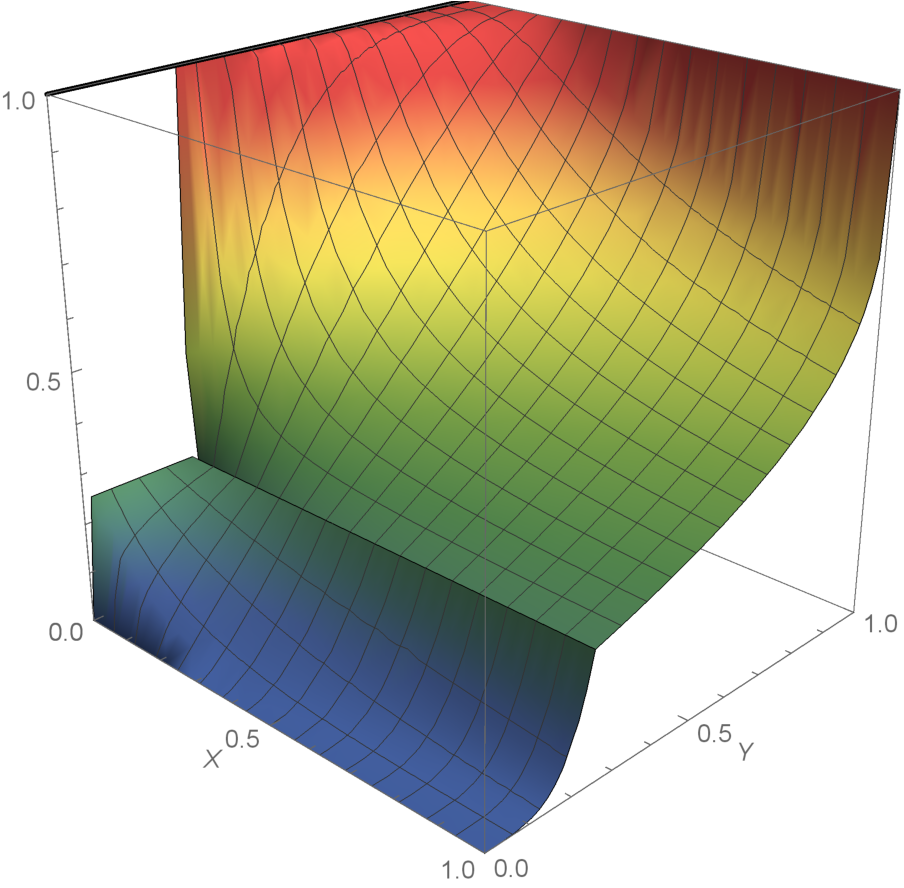
\includegraphics[width=4cm]{he1.pdf} }
		\subfloat[\centering $e=0.5$]{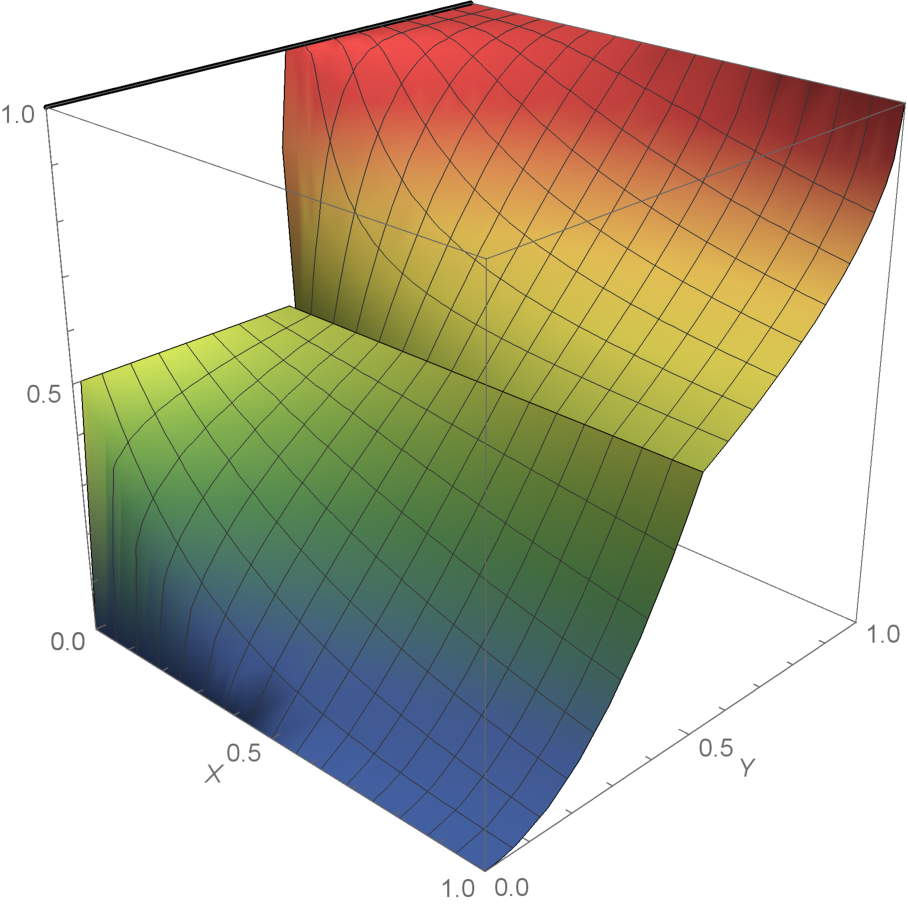
\includegraphics[width=4cm]{he2.pdf} }
		\subfloat[\centering $e=0.75$]{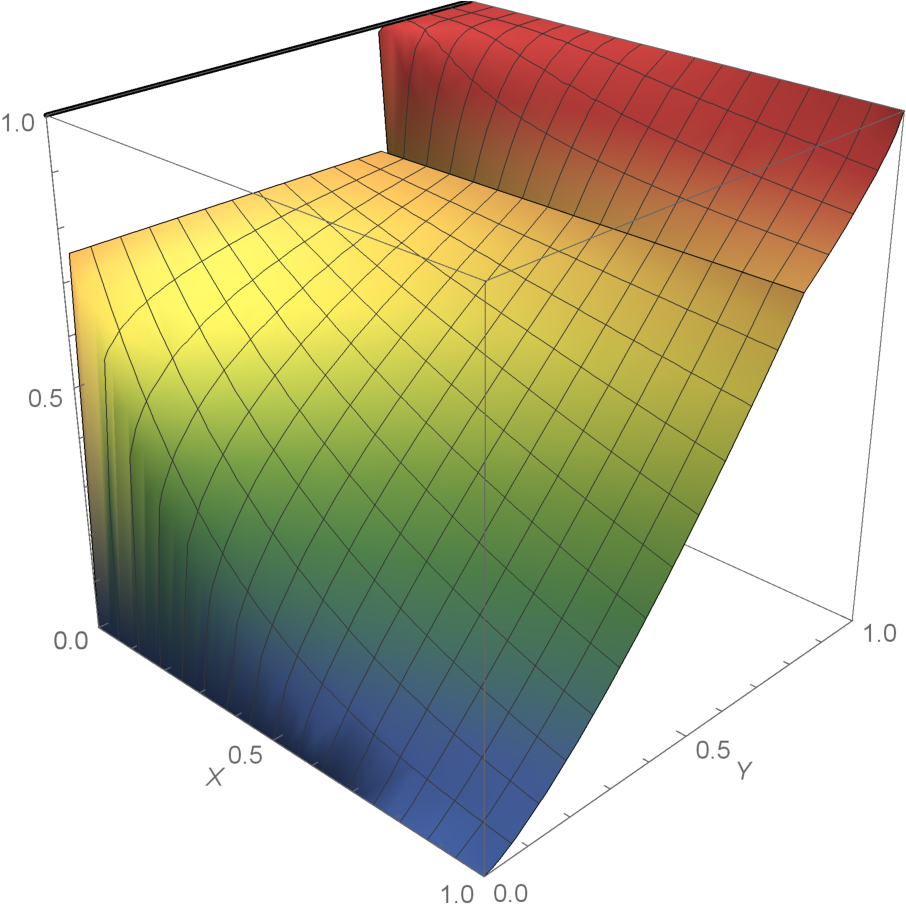
\includegraphics[width=4cm]{he3.pdf} }\\
		\caption[Plot of a generalized $(h,e)$-implication for different values of $e$.]{Plot of the generalized $(h,e)$-implication given by Equation (\ref{exemple(h,e)}) for different values of $e$.}\label{exempl(h,e)}
	\end{figure}
	\label{controlledincreasingness}
\end{example}

\subsection{Representation theorem}\label{subsection:representation_theorem}

Although prior to this study no axiomatic characterization of $(h,e)$-implications was available in the literature, in \cite{Massanet2013B} a representation theorem for this family was presented without the corresponding proof. In this section, we provide a proof for that result and we adjust it to the case of generalized $(h,e)$-implications.

\begin{theorem}\label{ThmRepresentacio(h,e)}
	Let $I:[0,1]^2 \to [0,1]$ be a binary function and $e \in (0,1)$. Then $I$ is a generalized $(h,e)$-implication with respect to $e$ if and only if there exist an $f$-generator and a $g$-generator with $g(1)=+\infty$ such that $I$ is given by
	\label{ThmRep(h,e)}
	\begin{equation}
		I(x,y) = \left\{ \begin{array}{lcl}
			1 &   \hbox{if}  & x=0, \\
			e \cdot f^{(-1)}\left(\frac{x}{e} \cdot f\left( \frac{y}{e}\right)\right)\ &  \hbox{if} & x>0,y\leq e, \\
			e+(1-e)\cdot g^{-1}\left( \frac{e}{x} \cdot g \left(\frac{y-e}{1-e}\right)\right) &  \hbox{if}  & x>0,y>e.
		\end{array}
		\right.
		\label{eq4}
	\end{equation}
	Moreover, in this case generators $h$, $f$ and $g$ are related in the following way
	
	$$f(x)=-h(e\cdot x), \quad \text{for all } x \in [0,1], \quad g(x)=h(e+(1-e)\cdot x), \quad \text{for all } x \in [0,1],$$
	
	$$ h(x) =  \left\{ \begin{array}{lcl}
		-f\left(\frac{x}{e} \right) &   \hbox{if}  & x \leq e, \\
		g\left(\frac{x-e}{1-e}\right) &  \hbox{if} & x>e.
	\end{array}
	\right.
	$$
\end{theorem}

\begin{proof}
	Let $I$ be a generalized $(h,e)$-implication with respect to $e$. We know that $h$ is a continuous and strictly increasing function with $h(e)=0$ and $h(1)=+\infty$. First of all, note that $f(x)=-h(ex)$ and $g(x)=h(e+(1-e)x)$ are $f$ and $g$-generators, respectively, since $f$ is a continuous and strictly decreasing function with $f(1)=-h(e)=0$ and $g$ is a continuous and strictly increasing function with $g(0)=h(e)=0$.  Note that since $h^{-1}$ is well defined on $[h(0), +\infty)$ with $h(0)<0$ then we have for all $ x \in [0, +\infty)$ that
	$$ f^{(-1)}(x) = \frac{h^{(-1)}(-x)}{e}, \quad g^{-1}(x) = \frac{h^{-1}(x)-e}{1-e}.$$
	For $x=0$ it is clear that $I(0,y)=1$ for all $y \in [0,1]$ and $I$ corresponds to Equation (\ref{eq4}) on these points. For the situation $x>0$ we will split the proof in two cases:
	\begin{itemize}
		\item If $x>0$ and $y \leq e$ then
		$$ e f^{(-1)} \left(\frac{x}{e}f\left(\frac{y}{e}\right) \right) = ef^{(-1)}\left(-\frac{x}{e}h(y)\right)= h^{(-1)} \left(\frac{x}{e}h(y) \right) = I(x,y).$$
		\item If $x>0$ and $ y > e$ then
		\begin{eqnarray*}
			e + (1-e) \cdot g^{-1}\left(\frac{e}{x}g\left(\frac{y-e}{1-e}\right)\right) &=& e + (1-e) \cdot \frac{h^{-1}\left( \frac{e}{x} h\left(e+(1-e) \frac{y-e}{1-e} \right)\right)-e}{1-e} \\
			&=& h^{-1} \left(\frac{e}{x}h(y) \right) = I(x,y).
		\end{eqnarray*}
	\end{itemize}
	For the reverse implication, let us consider $f$ and $g$-generators such that $I$ is given by Equation (\ref{eq4}). Consider
	$$h(x) = \left\{ \begin{array}{lcc}
		-f\left(\frac{x}{e} \right) &   \hbox{if}  & x \leq e, \\
		g \left( \frac{x-e}{1-e} \right) &  \hbox{if} & x>e .
	\end{array}
	\right.
	$$
	This function is continuous, strictly increasing, $h(e)=-f(1)=0$ and $h(1)=g(1)= + \infty$. Now, let us prove that $I = I^{h_g,e}$. Notice that
	\begin{eqnarray*}
		h^{(-1)}(x) &=& \left\{ \begin{array}{lcc}
			h^{-1}(x) &   \hbox{if}  & x \in [h(0), + \infty), \\
			0 &  \hbox{if} & x \in (- \infty, h(0)) ,
		\end{array}
		\right. \\
		&=&
		\left\{ \begin{array}{lcc}
			0 &  \hbox{if} & x \in (- \infty, -f(0)) , \\
			e \cdot f^{-1}(-x) &   \hbox{if}  & x \in [-f(0), 0], \\
			e+(1-e) \cdot g^{-1}(x) &  \hbox{if} & x \in (0, + \infty).
		\end{array}
		\right.
	\end{eqnarray*}
	Then, studying again two cases we have that
	\begin{itemize}
		\item If $x>0$ and $y \leq e$ then
		$$I^{h_g,e}(x,y)= h^{(-1)} \left(\frac{x}{e} h(y) \right) = h^{(-1)} \left(- \frac{x}{e} f \left( \frac{y}{e} \right) \right) = e \cdot f^{(-1)} \left(\frac{x}{e} f \left(\frac{y}{e} \right) \right)  = I(x,y).$$
		\item If $x>0$ and $y>e$ then
		\begin{eqnarray*}
			I^{h_g,e}(x,y) &=& h^{-1} \left(\frac{e}{x}h(y) \right) = h^{-1} \left(\frac{e}{x} g \left( \frac{y-e}{1-e}\right) \right) = e + (1-e) \cdot g^{-1} \left( \frac{e}{x} g \left( \frac{y-e}{1-e}\right) \right) \\
			&=&I(x,y).
		\end{eqnarray*}
	\end{itemize}
\end{proof}

The next example provides the construction of a generalized $(h,e)$-implication by using the threshold horizontal method given an $f$-generator and a $g$-generator with $g(1)=+\infty$.
\begin{example} Let us consider $e=\frac{1}{2}$ and the subsequent $f$ and $g$-generators
	
	$$ f(x)= - \ln \left( \frac{x}{2-x} \right), \quad g(x)=\ln \left( \frac{1+x}{1-x}\right).$$
	It is easy to check that the following functions are fuzzy implication functions
	$$I_1(x,y)=f^{(-1)}\left(\frac{x}{e} f(y)\right)= \frac{2y^{2x}}{(2-y)^{2x}+y^{2x}},$$
	$$ I_2(x,y)=\quad g^{-1}\left(\frac{e}{x}g(y)\right)=\frac{(1+y)^{\frac{1}{2x}}-(1-y)^{\frac{1}{2x}}}{(1+y)^{\frac{1}{2x}}+(1-y)^{\frac{1}{2x}}}.$$
	Then, a generalized $(h,e)$-implication is constructed from $I_1$ and $I_2$ by using the threshold horizontal method as described in Theorem \ref{ThmRepresentacio(h,e)}. Concretely, the $h$-generator corresponds to  
	$$h(x)=  \ln \left( \frac{x}{1-x}\right).$$
	We can see the construction method graphically in Figure \ref{thresholdimpl}.
	
	\begin{figure}[H]
		\centering
		\subfloat[\centering $I_1$]{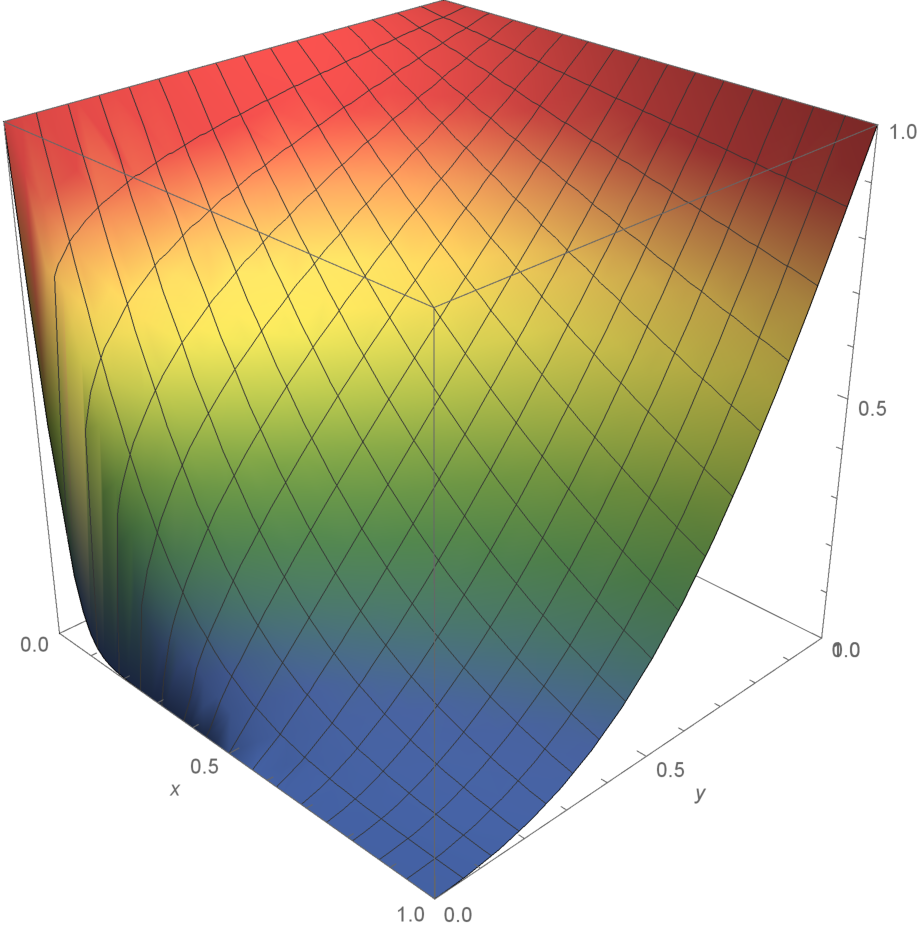
\includegraphics[width=4cm]{fe1.pdf} }
		\subfloat[\centering $I_2$]{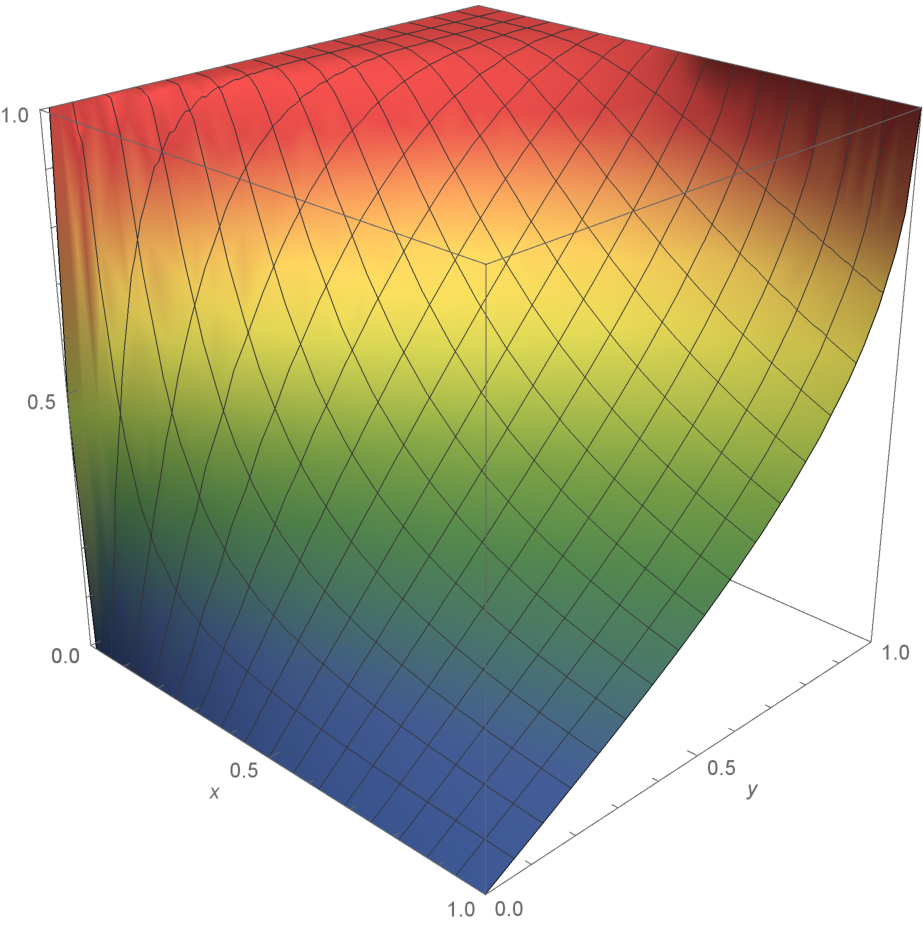
\includegraphics[width=4cm]{ge1.pdf} }
		\subfloat[\centering $I^{h,e} = I_{I_1-I_2}$]{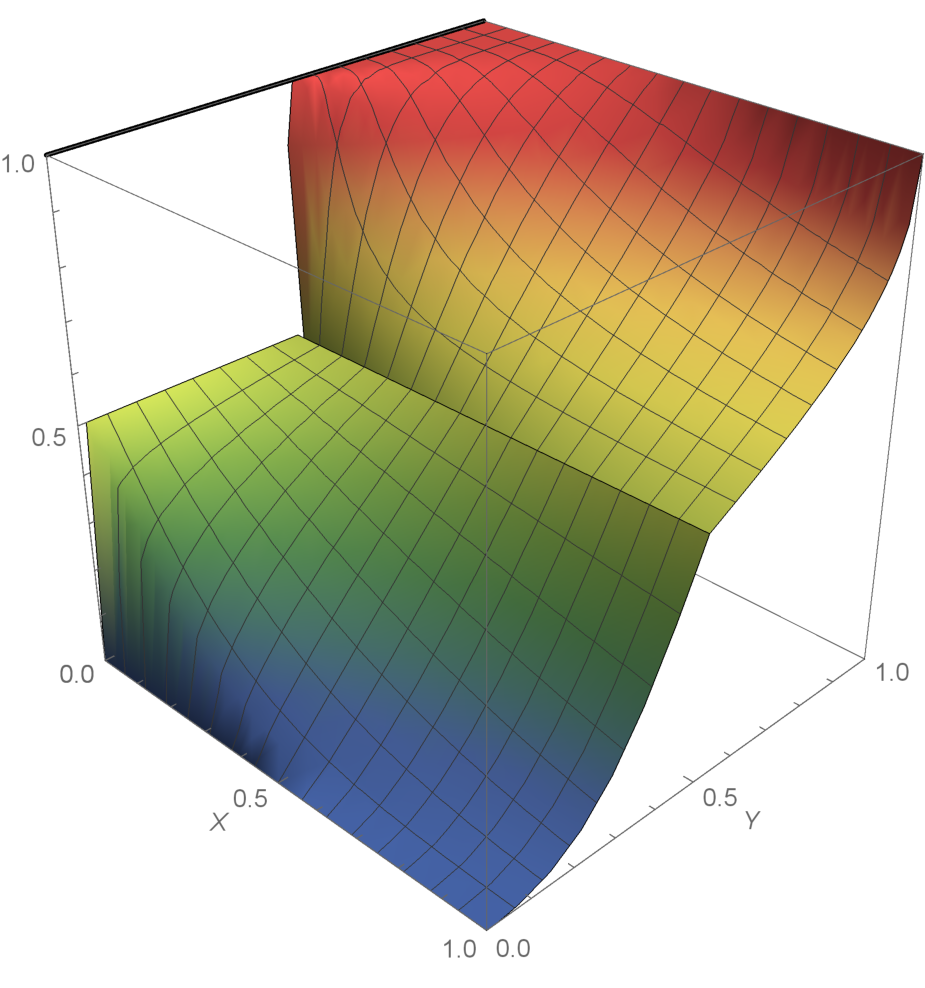
\includegraphics[width=4cm]{he.pdf} }\\
		
		\caption[Plot of a generalized $(h,e)$-implication constructed via the horizontal threshold method jointly with the two fuzzy implication functions that act as generators.]{Plot of a generalized $(h,e)$-implication with $e=\frac{1}{2}$ constructed via the horizontal threshold method jointly with the two fuzzy implication functions $I_1$, $I_2$ that act as generators.}\label{thresholdimpl}
	\end{figure}
	\label{ExempleRepresentació(h,e)}
\end{example}

Although Theorem \ref{ThmRepresentacio(h,e)} gives a useful description of the family of generalized $(h,e)$-implications, it is not an axiomatic characterization of this family, i.e., a characterization in terms of their own properties. For providing such result, a deeper study of this family is needed.

Let us recall that the characterization of $h$-implications presented in \cite{Massanet2012A} was written in terms of the threshold horizontal method, in particular $h$-implications are characterized by the fact that they are generated by an $f$-implication and a $g$-implication through the horizontal threshold method. In this case, the axiomatic characterization was not provided but it can be easily obtained by using the characterizations of Yager's implications presented in \cite{Massanet2012B}. For the case of generalized $(h,e)$-implications, it is straightforward to prove that if we consider an $f$-generator, the function $I_{f,e}:[0,1]^2 \to [0,1]$ defined by
$$I_{f,e}(x,y)=f^{(-1)}\left(\frac{x}{e}f(y)\right), \quad x,y \in [0,1],$$
with the understanding $+ \infty \cdot 0 = 0$ is a fuzzy implication function and if we consider a $g$-generator with $g(1)=+\infty$, the function $I_{g,e}:[0,1]^2 \to [0,1]$ defined by
$$I_{g,e}(x,y)=g^{(-1)}\left(\frac{e}{x}g(y)\right), \quad x,y \in [0,1],$$
with the understanding $\frac{1}{0}=+\infty$ and $+\infty \cdot 0 =+\infty$ is also a fuzzy implication function. Thus, Theorem \ref{ThmRepresentacio(h,e)} discloses that generalized $(h,e)$-implications are also characterized by the fact that they can be generated through the horizontal threshold method by the two new families of fuzzy implication functions just introduced.  Therefore, in order to obtain a characterization of $(h,e)$-implications, we have to study and characterize these two families.

In particular, $I_{f,e}$ and $I_{g,e}$ are fuzzy implication functions that belong to two families which are generalizations of the well-known Yager's implications, the $(f,g)$ and $(g,f)$-generated implications \cite{Massanet2013B}. In the next section we deeply study these two families.


\section{Generalized Yager's implications}\label{section:(f,g)&(g,f)}

In \cite{Massanet2013B} two new families of fuzzy implication functions, called the $(f,g)$ and $(g,f)$-generated implications, were defined as a generalization of the well-known Yager's $f$ and $g$-generated implications, respectively. In the definition of the $f$-generated implications one can consider the function $x$ as a particular case of a family of strictly increasing and continuous  functions defined as $g:[0,1] \to [0,+\infty]$ such that $g(0)=0$. The same happens to the role of $\frac{1}{x}$ as a concrete case of a continuous, strictly decreasing function $f:[0,1] \to [0,+\infty]$ such that $f(0)=+\infty$. In this section we recall the definitions and properties of these two families of fuzzy implication functions published in \cite{Massanet2013B}, providing the corresponding proofs and rectifying some  wrongly stated results.

\subsection{Generalization of Yager's $f$-generated implications}\label{subsection:f-generated}

First, we will study a generalization of the $f$-generated implications, generalizing the function $x$ in its definition as a strictly increasing function $g: [0,1] \to [0, + \infty]$ with $g(0)=0$.
\begin{definition}\label{def:(f,g)operations} Let $f:[0,1] \to [0,+\infty]$ be a strictly decreasing and continuous function with $f(1)=0$ and $g:[0,1] \to [0, + \infty]$ be a continuous and strictly increasing function with $g(0)=0$. The function $I_{f,g} : [0,1]^2 \to [0,1]$ defined by
	\begin{equation}
		I_{f,g}(x,y)=f^{(-1)}(g(x)f(y)),  \quad \text{for all } x,y \in [0,1],
		\label{expressiofg}
	\end{equation}
	\noindent with the understanding $0 \cdot (+\infty)=0$, is called an $(f,g)$-generated operation.
\end{definition}

\begin{remark} An initial difference between the family of $f$-generated implications and its generalization is that we need to consider the pseudo-inverse of $f$. This is because when $f(0) < + \infty$, $g(x) \cdot f(y)$ may be bigger than the initial value $f(0)$. Nevertheless, notice that Equation (\ref{expressiofg}) can also be written in the following form without explicitly using the pseudo-inverse of $f$:
	\begin{equation}
		I(x,y)=f^{-1}\Big(\min \Big\lbrace g(x)f(y),f(0) \Big\rbrace \Big), \quad \text{for all } x,y \in [0,1].
		\label{expressio2fg}
	\end{equation}
\end{remark}

An $(f,g)$-generated operation may not fulfill all the conditions in Definition \ref{defimp} and then it need not be a fuzzy implication function always.

\begin{theorem}\label{th:(f,g)implications} An $(f,g)$-operation $I_{f,g}$ is a fuzzy implication function if and only if one of the following conditions hold:
	\begin{enumerate}[label=(\roman*)]
		\item $f(0)=+\infty$.
		\item $f(0)< +\infty$ and $g(1) \geq 1$.
	\end{enumerate}
\end{theorem}
\begin{proof}
	First, we will consider that $I_{f,g}$ is a fuzzy implication function with $f(0)< + \infty$. In this case
	$$I_{f,g}(1,0)=f^{(-1)}(g(1)f(0)) =  \left\{ \begin{array}{lcc}
		f^{-1}(g(1)f(0)) &   \hbox{if}  & g(1) < 1, \\
		\\ 0 &   \hbox{if} & g(1)\geq 1.
	\end{array}
	\right.
	$$
	Since $I_{f,g}$ is a fuzzy implication function then it holds that $I_{f,g}(1,0)=0$ and hence, $g(1) \geq 1 $. Now, let us consider an $(f,g)$-operation satisfying (i) or (ii). The fact that $I_{f,g}$ is a fuzzy implication function can be seen from the following:
	\begin{itemize}
		\item Let $x_1,x_2,y \in [0,1]$ with $x_1 \leq x_2$. Since $g$ is strictly increasing we have that $g(x_1) \leq g(x_2)$. Now, since $f$ is strictly decreasing, $f^{(-1)}$ is decreasing and we get that
		$$ I_{f,g}(x_1,y) = f^{(-1)}(g(x_1)f(y)) \geq f^{(-1)}(g(x_2)f(y)) =I_{f,g}(x_2,y),$$
		and $I_{f,g}$ satisfies \Ione.
		\item Consider $x,y_1,y_2 \in [0,1]$ with $y_1 \leq y_2$ then, again by the strictly decreasing nature of $f$, $f^{(-1)}$ is decreasing, and hence, we have
		\begin{eqnarray*}
			f(y_1) \geq f(y_2) &\Rightarrow& g(x) \cdot f(y_1) \geq g(x) \cdot f(y_2) \\
			&\Rightarrow & f^{(-1)}(g(x) \cdot f(y_1)) \leq f^{(-1)}(g(x) \cdot f(y_2)) \\
			&\Rightarrow & I_{f,g}(x,y_1) \leq I_{f,g}(x,y_2),
		\end{eqnarray*}
		and $I_{f,g}$ satisfies \Itwo.
		\item $I_{f,g}(0,0)=f^{(-1)}(g(0)f(0))=f^{(-1)}(0)=1$.
		\item $I_{f,g}(1,1)=f^{(-1)}(g(1)f(1))=f^{(-1)}(0)=1$.
		\item $I_{f,g}(1,0)=f^{(-1)}(g(1)f(0))$ and we have two cases. If $f(0)= + \infty$ then $I_{f,g}(1,0)=f^{-1}(+\infty)=0$. Otherwise, if $f(0) < +\infty$ and $g(1) \geq 1$ then, $f(0)g(1) \geq f(0)$ and $I_{f,g}(1,0)=0$.
	\end{itemize}
\end{proof}
When an $(f,g)$-operation fulfills Definition \ref{defimp}, we will use the nomenclature $(f,g)$-implication and we will call an admissible pair of generators to the pair of functions $(f,g)$.
\begin{remark}\label{Remark:Comparison(f,g)}
	In \cite{XieLiu2013} a similar approach to provide a generalization of Yager's $f$-implications was considered. In this case, the authors consider the fuzzy implication function given by $I_{f,g}(x,y)=f^{(-1)}(g(x)f(y))$ where  $f$ is an $f$-generator and $g:[0,1] \to [0,1]$ is an increasing function satisfying $g(0)=0$ and $g(1)=1$. In this case, they consider functions $g$ which are not necessarily continuous but with $g(1)=1$. Our approach restricts to the case when $g$ is continuous but allows any value in $(0,+\infty)$ of $g(1)$ whenever $f(0)=+\infty$ and any value $g(1) \geq 1$ whenever $f(0)<+\infty$. Clearly, the two families intersect when we consider a continuous, strictly decreasing function $g$ with $g(1)=1$. Moreover, by Remark 2.1 in \cite{XieLiu2013}, in this particular case the resulting $(f,g)$-implications are in fact $\phi$-conjugated of $f$-generated implications with $f$ generator given by $f \circ g^{-1}$ and $\varphi=g$.
\end{remark}
The next result shows that it is enough to consider the pairs $(f,g)$ of admissible generators such that $f(0)=+\infty$ or $f(0)=1$.
\begin{proposition} Let $I_{f,g}$ be a fuzzy implication function with $f(0) < +\infty$, then there exists a function $f_1$ with $f_1(0)=1$ such that $(f_1,g)$ is an admissible pair of generators and $I_{f,g}=I_{f_1,g}$.
\end{proposition}
\begin{proof}
	Let $I_{f,g}$ be a fuzzy implication function with $f(0) < + \infty$ and consider $f_1(x)=\frac{f(x)}{f(0)}$. Then, $(f_1,g)$ is an admissible pair of generators with $f_1(0)=\frac{f(0)}{f(0)}=1$ and since $f_1^{-1}(x) = f^{-1}(xf(0))$ then
	\begin{eqnarray*}
		I_{f_1,g}(x,y)&=&f_1^{(-1)}\left(g(x)f_1(y)\right) = f_1^{(-1)}\left(g(x)\frac{f(y)}{f(0)}\right) =  f_1^{-1} \left( \min \left\lbrace g(x)\frac{f(y)}{f(0)},f_1(0)\right \rbrace\right) \\
		&=& f^{-1}\left( \min \{ g(x)f(y), f(0) \}\right) = I_{f,g}(x,y).
	\end{eqnarray*}
\end{proof}


Then next proposition shows that the $(f,g)$-generated implications have non-trivial zero region for some choice of generators.


\begin{proposition} Let $(f,g)$ be an admissible pair of generators. Then the following statements hold:
	\begin{enumerate}[label=(\roman*)]
		\item If $g(1) < f(0) = + \infty$, then $I_{f,g}(x,y)=0$ if and only if $y=0<x$.
		\item If $g(1)=f(0)= + \infty$, then $I_{f,g}(x,y)=0$ if and only if $y<x=1$ or $y=0<x$.
		\item If $f(0)< + \infty$, then $I_{f,g}(x,y)= 0$ if and only if $g(x) \geq 1$ and $ y \leq f^{-1}\left(\frac{f(0)}{g(x)}\right)$.
	\end{enumerate}
\end{proposition}
\begin{proof} \hspace{0.5cm}
	\begin{enumerate}[label=(\roman*)]
		\item Let us assume that $g(1)<f(0)= + \infty$ then $f^{(-1)}=f^{-1}$. Hence, for every $x,y \in [0,1]$ we have that 
		$$I_{f,g}(x,y)=f^{-1}(g(x)f(y))=0 \Leftrightarrow g(x)f(y)=f(0)=+\infty.$$
		However, we know that $g(x) \leq g(1) < + \infty$ and then, the only possibility is $f(y)=+\infty$ and $g(x) \not = 0$. Consequently, $y=0<x$.
		\item Again we have that $f^{(-1)}=f^{-1}$ and then,
		$$I_{f,g}(x,y)=0 \Leftrightarrow g(x)f(y)= + \infty.$$
		Therefore, $g(x)=+ \infty$ and $f(y)>0$ or, $g(x)>0$ and $f(y)=+\infty$. Hence, the results follows.
		\item Consider $x,y \in [0,1]$ then
		$$I_{f,g}(x,y)=0 \Leftrightarrow f^{(-1)}(g(x)f(y))=0 \Leftrightarrow g(x)f(y) \in [f(0), + \infty).$$
		Now, since $f$ is strictly decreasing, $f(y) \leq f(0)$ for all $ y \in [0,1]$ and then necessarily $g(x) \geq 1$. Finally,
		$$g(x)f(y)\geq f(0) \Leftrightarrow f(y) \geq \frac{f(0)}{g(x)} \Leftrightarrow y \leq f^{-1}\left(\frac{f(0)}{g(x)}\right).$$
	\end{enumerate}
\end{proof}


On the other hand, the next proposition shows that the region where the $(f,g)$-generated implications take the value 1 is independent of their generators.

\begin{proposition}\label{onezonefg} Let $(f,g)$ be an admissible pair of generators. Then $I_{f,g}(x,y)=1$ if and only if $x=0$ or $y=1$.
\end{proposition}
\begin{proof} Let $(f,g)$ be an admissible pair of generators and $x,y \in [0,1]$. Then,
	\begin{eqnarray*}
		I_{f,g}(x,y)=1 & \Leftrightarrow & f^{(-1)}(g(x)f(y))=1 \Leftrightarrow g(x)f(y)=0 \\
		& \Leftrightarrow & g(x)=0 \text{ or } f(y)=0 \Leftrightarrow x=0 \text{ or } y=1.
	\end{eqnarray*}
\end{proof}
The determination of the one region obtained in the previous proposition is a property of fuzzy implication functions deeply studied in \cite{Bustince2013} where it is explained that the property ($I(x,y)=1 \Leftrightarrow x=0 \hbox{ or } y=1$) is very important for the definition of strong equality indices. Consequently, $(f,g)$-implications could be used to generate strong equality indices. Also, in \cite{Massanet2012B} this property plays a crucial role in the characterization of $f$-generated implications.

From the previous proposition, the following result is straightforward.

\begin{corollary} Let $(f,g)$ be an admissible pair of generators. Then the $(f,g)$-implication $I_{f,g}$ does not satisfy either \IP or \OP.
\end{corollary}

The next proposition studies under which conditions \NP is satisfied by the $(f,g)$-generated implications. This property is satisfied by many of the most well-known families and therefore, to determine when $(f,g)$-implications fulfill \NP is a necessary step for forthcoming studies on the intersections of this family with other existing families.

\begin{proposition}\label{prop:(f,g):(NP)}
	 Let $(f,g)$ be an admissible pair of generators. Then $I_{f,g}$ satisfies \NP if and only if $g(1)=1$.
\end{proposition}
\begin{proof}
	Consider $(f,g)$ an admissible pair of generators. It is straightforward to prove that if $g(1)=1$ then $I_{f,g}$ satisfies \NP, so let us prove the reverse implication. If $I_{f,g}$ satisfies \NP then
	$$f^{(-1)}(g(1)f(y))=I_{f,g}(1,y)=y, \quad \text{for all } y \in [0,1].$$
	Thus, $g(1)<+\infty$. Now, since $f$ is strictly decreasing and continuous with $f(1)=0$ we can choose $y \in (0,1)$ such that $g(1)f(y)< f(0)$ and then
	$$
	y=I_{f,g}(1,y)=f^{(-1)}(g(1)f(y))  \Rightarrow  g(1)f(y)=f(y) \Rightarrow  g(1)=1.
	$$
\end{proof}

The following result studies the natural negation of these fuzzy implication functions. The properties of the natural negation play an important role in many characterization results of fuzzy implication functions.
\begin{proposition}\label{negationfg} Let $(f,g)$ be an admissible pair of generators. Then the following properties hold:
	\begin{enumerate}[label=(\roman*)]
		\item If $f(0)=+\infty$, then the natural negation $N_{I_{f,g}}$ is the G\"odel or least negation $\NDOne$.
		\item If $f(0)<+\infty$, then the natural negation $N_{I_{f,g}}$ is given by
		$$N_{I_{f,g}}(x)= \left\{ \begin{array}{lcc}
			f^{-1}(g(x)f(0)) &   \hbox{if}  & g(x) < 1, \\
			0 &  \hbox{if} & g(x)\geq 1.
		\end{array}
		\right.
		$$
		\item The natural negation $N_{I_{f,g}}$ is strict if and only if $f(0) < +\infty$ and $g(1)=1$.   
	\end{enumerate}
\end{proposition}

\begin{proof}
	\begin{enumerate}[label=(\roman*)]
		\item If $f(0)=+\infty$, then $f^{(-1)}=f^{-1}$ and for every $x \in [0,1]$ we get
		\begin{eqnarray*}
			N_{I_{f,g}}(x)&=&f^{-1}(g(x)f(0)) = \left\{ \begin{array}{lcc}
				f^{-1}(+ \infty) &   \hbox{if}  & g(x) \not = 0, \\
				f^{-1}(0) &  \hbox{if} & g(x) = 0,
			\end{array}
			\right.
			=
			\left\{ \begin{array}{lcc}
				0 &   \hbox{if}  & x>0, \\
				1 &  \hbox{if} & x=0,
			\end{array}
			\right. \\
			&=& \NDOne(x).
		\end{eqnarray*}
		\item If $f(0) < + \infty$ then we have
		\begin{eqnarray*}
			N_{I_{f,g}}(x)&=&f^{(-1)}(g(x)f(0)) =            \left\{ \begin{array}{lcc}
				f^{-1}(g(x)f(0)) &   \hbox{if}  & g(x)f(0) < f(0), \\
				0 &  \hbox{if} & g(x)f(0)\geq f(0),
			\end{array}
			\right. \\
			&=&
			\left\{ \begin{array}{lcc}
				f^{-1}(g(x)f(0)) &   \hbox{if}  & g(x) < 1, \\
				0 &  \hbox{if} & g(x)\geq 1.
			\end{array}
			\right.
		\end{eqnarray*}
		\item If $f(0) < + \infty$ and $g(1)=1$ it is straightforward from Point (ii) that $N_{I_{f,g}}$ is a continuous function since it is the composition of real continuous functions. Consider $x_1<x_2$, by the strictly increasing nature of $g$, we have that $g(x_1)f(0) < g(x_2)f(0)$. Now, since $f$ is strictly decreasing, $f^{-1}$ is strictly decreasing in $[0,f(0)]$ and we get that
		$$N_{I_{f,g}}(x_1)=f^{-1}(g(x_1)f(0))>f^{-1}(g(x_2)f(0))=N_{I_{f,g}}(x_2).$$
		Hence, $N_{I_{f,g}}$ is strictly decreasing and therefore, it is a strict fuzzy negation. Reciprocally, Points (i) and (ii) show that the obtained natural negations are not strictly decreasing when $f(0)=+\infty$ or when $f(0)<+\infty$ and $g(1)>1$.
	\end{enumerate}
\end{proof}

At this point, we analyze the discontinuity points of the $(f,g)$-generated implications, which can be $(0,0)$ or  $(1,1)$.

\begin{proposition}\label{prop:(f,g):continuity} 
	Let $(f,g)$ be an admissible pair of generators. Then $I_{f,g}$ is continuous everywhere except  at point $(0,0)$ when $f(0)=+\infty$ or at point $(1,1)$ when $g(1)=+\infty$.
\end{proposition}
\begin{proof}
	Let $(f,g)$ be an admissible pair of generators, then by definition $I_{f,g}$ is continuous on each $(x,y) \in [0,1]^2$ by being the composition of real continuous functions except for the cases when ($g(x)=0$ and $f(y)=+\infty$) or ($g(x)=+\infty$ and $f(y)$=0), since in these situations we have considered the convention $0 \cdot (+\infty)=0$.	These two situations correspond to the following two cases:
	\begin{itemize}
		\item If $x=y=0$ and $f(0)=+\infty$, then by (i)-Proposition \ref{negationfg}, the natural negation of $I_{f,g}$ is not continuous on $x=0$ and therefore $I_{f,g}$ is non-continuous on $(0,0)$.
		\item If $x=y=1$ and $g(1)=+\infty$ then
		$$I_{f,g}(1,y)=f^{(-1)}(+ \infty \cdot f(y)) = \left\{ \begin{array}{lcc}
			f^{-1}(0) &   \hbox{if}  & y=1, \\
			0 &  \hbox{if} & y<1,
		\end{array}
		\right.
		= \left\{ \begin{array}{lcc}
			1 &   \hbox{if}  & y=1, \\
			0 &  \hbox{if} & y<1.
		\end{array}
		\right.
		$$
		Hence, we have that
		$$\lim_{y \to 1^{-}} I_{f,g}(1,y)=0 \not = 1= I_{f,g}(1,1),$$
		and $I_{f,g}$ is not continuous on $(1,1)$.
	\end{itemize}
\end{proof}


Consequently, there are members of the family which are continuous in the whole domain. Namely, when $f(0)<+\infty$ and $1 \leq g(1) < + \infty$.

Finally, we present two results that determine completely when the $(f,g)$-generated implications satisfy \EP or \LI.

\pagebreak

\begin{proposition}\label{EPfg} 
	Let $(f,g)$ be an admissible pair of generators. Then the following statements are equivalent:
	\begin{enumerate}[label=(\roman*)]
		\item $I_{f,g}$ satisfies \EP.
		\item $f(0)=+\infty$ or ($f(0)<+\infty$ and $g(1)=1$).
	\end{enumerate}
\end{proposition}
\begin{proof}
	Assume that $I_{f,g}$ is an $(f,g)$-implication with $f(0)<+\infty$, $g(1) \geq 1$ and such that it satisfies \EP. Since $g$ is a strictly increasing and continuous function with $g(0)=0$, we can find an $x_0 \in (0,1)$ such that $g(x_0) \in (0,1)$. Then,
	$$I_{f,g}(x_0,I_{f,g}(1,0)) = I_{f,g}(x_0,0)=f^{-1}(g(x_0)f(0)).$$
    $$I_{f,g}(1,I_{f,g}(x_0,0)) = I_{f,g}(1,f^{-1}(g(x_0)f(0)))=f^{(-1)}(g(1)g(x_0)f(0)).$$
    In this case, $0 < f^{-1}(g(x_0)f(0)) < 1$. Thus, since $I_{f,g}$ satisfies \EP necessarily $g(1)=1$. For the reverse implication we have two cases:
	\begin{itemize}
		\item If $f(0)=+ \infty$ then $f^{(-1)}=f^{-1}$ and we obtain
		\begin{eqnarray*}
			I_{f,g}(x,I_{f,g}(y,z))&=& f^{-1}(g(x) \cdot (f \circ f^{-1})(g(y)f(z))) = f^{-1}(g(x)g(y)f(z)) \\
			&=& f^{-1} ( g(y) \cdot (f\circ f^{-1}) (g(x)f(z))= I_{f,g}(y,I_{f,g}(x,z)).
		\end{eqnarray*}
		Hence, $I_{f,g}$ satisfies \EP.
		
		\item If $f(0)< + \infty$ and $g(1)=1$, since $g$ is strictly increasing and $f$ strictly decreasing 
		$$ g(x)f(y) \leq f(y) \leq f(0) ~~ \text{ for all } ~~ x,y \in [0,1].$$
		Thus, in this case we have that $I_{f,g}(x,y)=f^{-1}(g(x)f(y))$ for all $x,y \in [0,1]$ and, similarly to the previous point, we can prove that $I_{f,g}$ satisfies \EP. \qedhere
		
	\end{itemize}
\end{proof}

\begin{proposition}\label{prop:(f,g):(LI)} 
	Let $(f,g)$ be an admissible pair of generators and $T$ a t-norm. Then the following statements are equivalent:
	\begin{enumerate}[label=(\roman*)]
		\item The couple of functions $I_{f,g}$ and $T$ satisfy \LI.
		\item $g(1)=1$ and $T=(\TP)_g$, i.e., $T(x,y)=g^{-1}(g(x)g(y))$ for all $x,y \in [0,1]$.
	\end{enumerate}
\end{proposition}

\begin{proof}
	First, let us consider $g(1)=1$ and $T(x,y)=g^{-1}(g(x)g(y))$, then  $g(x) \in [0,1]$ for all $x\in [0,1]$ and we have that
	$$I_{f,g}(T(x,y),z)=f^{(-1)}(g(x)g(y)f(z)) = f^{-1}(g(x)g(y)f(z)).$$
	On the other hand, by the strictly decreasing nature of $f$ we have that
	$$g(x)f(y) \leq f(y) \leq f(0) \text{ for all } x,y \in [0,1].$$
	Then $I_{f,g}(x,y)=f^{-1}(g(x)f(y))$ for all $x,y \in [0,1]$ and we get
	$$I_{f,g}(x,I_{f,g}(y,z))=f^{-1}(g(x)g(y)f(z)).$$
	Hence, $I_{f,g}$ satisfies \LI with respect to $(\TP)_g$.\\
	Now, let us assume that $I_{f,g}$ satisfies \LI with respect to a certain t-norm $T$, we know that $I_{f,g}$ also satisfies \EP. Then, by Proposition \ref{EPfg} $f(0) = + \infty$ or ($g(1)=1$ and $f(0) < + \infty$) and we have two cases:
	\begin{itemize}
		\item If $f(0)= + \infty$ we know that $f^{(-1)} = f^{-1}$. Therefore, for all $x,y,z \in [0,1]$ we have that
		\begin{eqnarray*}
			I_{f,g}(T(x,y),z)=I_{f,g}(x,I_{f,g}(x,y)) & \Leftrightarrow &   f^{-1}(g(T(x,y))f(z))= f^{-1}(g(x)g(y)f(z)) \\
			&\Leftrightarrow & g(T(x,y))=g(x)g(y).
		\end{eqnarray*}
		Now, since $T$ is a t-norm, for all $ y \in (0,1)$ we have
		$$g(y)=g(T(1,y))=g(1)g(y),$$
		hence, $g(1)=1$. Then $g(x)g(y) \in [0,1]$ and $T(x,y)=g^{-1}(g(x)g(y))$ for all $x,y \in [0,1]$.
		\item On the other hand, if $f(0) < +\infty$ and $g(1)=1$ then we know from the proof of Proposition \ref{EPfg} that in this case $I_{f,g}(x,y)=f^{-1}(g(x)f(y))$ and from the equality
		$$ I_{f,g}(T(x,y),z)=I_{f,g}(x,I_{f,g}(y,z)) \Leftrightarrow g(T(x,y))f(z) = g(x)g(y)f(z),$$
		we obtain the result.
	\end{itemize} 
\end{proof}

It is worth noting that if $g(1) > 1$ then these implications do not satisfy the law of importation with any t-norm, which is a huge difference from the particular case of the $f$-generated implications whose characterization in \cite{Massanet2012B} is based on this property. Moreover, note that this family of fuzzy implication functions provides new examples of functions satisfying the exchange principle but not the law of importation with respect to any t-norm. 

\subsection{Generalization of Yager's $g$-generated implications}\label{subsection:g-generated}

Now, we introduce a similar generalization for the $g$-generated implications by replacing the role of $\frac{1}{x}$ in their definition for a continuous and strictly decreasing function $f:[0,1] \to [0, + \infty]$ with $f(0)=+ \infty$.
\begin{definition}\label{def:(g,f)operations} Let $g:[0,1] \to [0, + \infty]$ be a strictly increasing and continuous function with $g(0)=0$ and $f:[0,1] \to [0, + \infty]$ be a continuous and strictly decreasing function with $f(0)= + \infty$. The function $I:[0,1]^2 \to [0,1]$ defined by
	\begin{equation}
		I_{g,f}(x,y)=g^{(-1)}(f(x)g(y)), ~~ x,y \in [0,1],
		\label{expressio1gf}
	\end{equation} 
	\noindent with the understanding $0 \cdot (+\infty) = + \infty$ and $\frac{1}{0}=+\infty$, is called a $(g,f)$-generated operation.
\end{definition}

\begin{remark} 	The use of the pseudo-inverse in Equation (\ref{expressio1gf}) can be avoided using the following expression
	\begin{equation}\label{expressio2gf}
		I_{g,f}(x,y)=g^{-1}(\min \{f(x)g(y),g(1)\}) ~,~ x,y \in [0,1].
	\end{equation}
\end{remark}
As in the case of the $(f,g)$-operations, not for all pairs of functions $(g,f)$ under the previous conditions we obtain a fuzzy implication function.

\begin{theorem}\label{th:(g,f)implications} A $(g,f)$-operation $I_{g,f}$ is a fuzzy implication function if and only if, one of the following conditions hold:
	\begin{enumerate}[label=(\roman*)]
		\item $g(1)= + \infty$.
		\item $g(1)< + \infty$ and $f(1) \geq 1$.
	\end{enumerate}
\end{theorem}
\begin{proof}
	First, let us assume that $I_{g,f}$ is a fuzzy implication function such that $g(1) < + \infty$. In this case, we have
	$$1=I_{g,f}(1,1)=g^{(-1)}(f(1)g(1))=  \left\{ \begin{array}{lcc}
		g^{-1}(f(1)g(1)) &   \hbox{if}  & f(1) < 1, \\
		1 &  \hbox{if} & f(1)\geq 1.
	\end{array}
	\right.
	$$
	Hence, necessarily $f(1) \geq 1$. On the other hand, consider a $(g,f)$-operation satisfying (i) or (ii). 
	\begin{itemize}
		\item Let $x_1,x_2,y \in [0,1]$ with $x_1 \leq x_2$. Since $f$ is strictly decreasing then $f(x_1) \geq f(x_2)$. Now, since $g$ is strictly increasing, $g^{(-1)}$ is increasing and we get
		$$ I_{g,f}(x_1,y)=g^{(-1)}(f(x_1)g(y)) \geq g^{(-1)}(f(x_2)g(y)) = I_{g,f}(x_2,y),$$
		and $I_{g,f}$ satisfies \Ione.
		
		\item Consider $x,y_1,y_2 \in [0,1]$ with $y_1 \leq y_2$, since $g$ and $g^{(-1)}$ are increasing then $g(y_1) \leq g(y_2)$ and we have that
		$$I_{g,f}(x,y_1)=g^{(-1)}(f(x)g(y_1)) \leq g^{(-1)}(f(x)g(y_2)) = I_{g,f}(x,y_2),$$
		then $I_{g,f}$ satisfies \Itwo.
		\item $I_{g,f}(0,0)=g^{(-1)}(f(0)g(0))=g^{(-1)}(+\infty \cdot 0) = g^{(-1)}(+\infty)=1$.
		\item $I_{g,f}(1,1)=g^{(-1)}(g(1)f(1))$ and we need to distinguish two cases. If $g(1)=+ \infty$ then we have that $I_{g,f}(1,1)=g^{-1}(+ \infty)=1$. On the other hand, if $g(1) < +\infty$ and $f(1) \geq 1$ then $g(1)f(1) \geq g(1)$ and we get that $I_{g,f}(1,1)=1$.
		\item $I_{g,f}(1,0)=g^{(-1)}(f(1)g(0))=g^{(-1)}(f(1) \cdot 0 )=g^{(-1)}(0)=0$.
	\end{itemize}
\end{proof}
Whenever a $(g,f)$-operation satisfies the properties given in Definition \ref{defimp}, we will call it a $(g,f)$-implication with its associated admissible pair of generators  $(g,f)$.
\begin{remark}
	In \cite{PeiZhu2017} a similar approach was considered. The authors define the family of fuzzy implication functions given by $I(x,y)=g^{(-1)}(f(x)g(y))$ where $f:[0,1] \to [1,+\infty]$ is a continuous, decreasing function satisfying $f(0)=+\infty$, $f(1)=1$ and $g$ is a $g$-generator.  In this case, they consider functions $f$ not necessarily strictly decreasing but with $f(1)=1$. In our case, we consider functions $f$ which are strictly decreasing, but we allow any value in $(0,+\infty)$ of $f(1)$ whenever $g(1)=+\infty$ and $f(1) \geq 1 $ when $g(1)< + \infty$. Then, the two families are not equivalent but they have intersection when we consider a continuous, strictly decreasing function with $f(1)=1$. However, since the two families are very similar, one can verify that the conditions which ensure that the two families fulfill a certain property are very similar in the two cases.
\end{remark}
In a similar way as in the $(f,g)$-implications, for $(g,f)$-implications it is only necessary to consider those pairs of admissible generators $(g,f)$ such that $g(1)=1$ or $g(1)=+\infty$, as it is shown in the following result.
\begin{proposition}\label{generadorfinitgf} Let $I_{g,f}$ be a fuzzy implication function with $g(1) < +\infty$, then there exists a function $g_1$ with $g_1(1)=1$ such that $(g_1,f)$ is an admissible pair of generators and $I_{g,f}=I_{g_1,f}$.
\end{proposition}
\begin{proof}
	Let $I_{g,f}$ be a fuzzy implication function with $g(1) < +\infty$. If we consider $g_1(x)=\frac{g(x)}{g(1)}$ then $(g_1,f)$ is also an admissible pair of generators with $g_1(1)=1$ . Moreover, $g_1^{-1}(x)=g^{-1}(xg(1))$ and we have that
	\begin{eqnarray*}
		I_{g_1,f}(x,y)&=&g_1^{(-1)}(f(x)g_1(y))=g_1^{(-1)}\left(f(x)\frac{g(y)}{g(1)}\right) = g_1^{-1} \left(\min \left\lbrace f(x)\frac{g(y)}{g(1)},g_1(1)\right\rbrace\right)\\
		&=&  g^{-1}(\min \{ f(x)g(y),g(1) \} )=I_{g,f}(x,y).
	\end{eqnarray*}
\end{proof}
Now, we will follow a similar approach to the previous section in order to study the properties of these fuzzy implication functions. Let us start by studying the region where the $(g,f)$-implications take value 1. Notice that $(g,f)$-implications may have a non-trivial 1 region.
\begin{proposition}\label{zona1gf} Let $(g,f)$ be an admissible pair of generators. Then the following statements hold:
	\begin{enumerate}[label=(\roman*)]
		\item If $g(1)= + \infty$, then $I_{g,f}(x,y)=1 \Leftrightarrow x=0$ or $y=1$.
		\item If $g(1) < + \infty$, then $I_{g,f}(x,y)=1 \Leftrightarrow y \geq g^{-1}\left(\frac{g(1)}{f(x)}\right)$.
	\end{enumerate}
\end{proposition}
\begin{proof}\hspace{0.5cm}
	\begin{enumerate}[label=(\roman*)]
		\item If $g(1)=+\infty$ we know that $g^{(-1)}=g^{-1}$ and then for any $x,y \in [0,1]$ we have
		\begin{eqnarray*}
			I_{g,f}(x,y)=g^{-1}(f(x)g(y))=1 & \Leftrightarrow & f(x)g(y)=g(1)=+ \infty \\  & \Leftrightarrow &  f(x) = + \infty \text{ or } g(y)= + \infty \\
			& \Leftrightarrow &x=0 \text{ or } y=1.
		\end{eqnarray*}
		\item If $g(1) < + \infty$, then by the definition of $g^{(-1)}$, for every $x,y \in [0,1]$ we know that
		$$I_{g,f}(x,y)=g^{(-1)}(f(x)g(y))=1 \Leftrightarrow f(x)g(y) \geq g(1) \Leftrightarrow y \geq g^{-1}\left(\frac{g(1)}{f(x)}\right).$$
	\end{enumerate}
\end{proof}

From the previous result we can see that unlike the $(f,g)$-implications, $(g,f)$-implications satisfy the identity principle in certain cases.

\begin{corollary}\label{cor:(g,f)(IP)}
Let $(g,f)$ be an admissible pair of generators. Then $I_{g,f}$ satisfies {\bf (IP)} if and only if $g(1) < + \infty$ and $f(x) \geq \frac{g(1)}{g(x)}$ for all $x \in [0,1]$.
\end{corollary}

On the other hand, the following proposition study the region where these fuzzy implication functions attain value zero. This result has been corrected since in \cite[Proposition 9]{Massanet2013B} the case when $f(1)=0$ was not contemplated.

\begin{proposition} Let $(g,f)$ be an admissible pair of generators. Then the following statements hold:
	\begin{enumerate}[label=(\roman*)]
		\item If $f(1)>0$, then $I_{g,f}(x,y)=0$ if and only if $x>0$ and $y=0$.
		\item If $f(1)=0$ and $g(1)=+\infty$, then $I_{g,f}(x,y)=0$ if and only if ($x=1$ and $y<1$) or ($x>0$ and $y=0$).
	\end{enumerate}
\end{proposition}
\begin{proof}
	Consider $x,y \in [0,1]$ then
	$$I_{g,f}(x,y)=g^{(-1)}(f(x)g(y))=0 \Leftrightarrow f(x)g(y)=0.$$
	Taking into account that either $g(1)=+\infty$ or $g(1)<+\infty$ and $f(1) \geq 1$ and the understanding $0 \cdot (+\infty)=+\infty$ we obtain the result.
\end{proof}


From the last result it is straightforward to see that these fuzzy implication functions satisfy that their natural negation is \NDOne. Then, the natural negation of $(g,f)$-implications is independent of their generators.

\begin{corollary} Let $(g,f)$ be an admissible pair of generators. Then the natural negation $N_{I_{g,f}}$ is the G\"odel or least fuzzy negation \NDOne.
	\label{negationgf}
\end{corollary}

The next result reflects that, as in the case of {\bf (IP)}, the property {\bf (OP)} can be satisfied by $(g,f)$-implications under certain restrictions on their generators. This result has been corrected with respect to the original one 
(\cite[Proposition 11]{Massanet2013B}) since the expression in Point (iii) was not correct. Moreover, we explicitly find the constant in Point (ii).

\begin{proposition}\label{prop:(g,f)(OP)} 
Let $(g,f)$ be an admissible pair of generators. Then the following statements are equivalent:
	\begin{enumerate}[label=(\roman*)]
		\item $I_{g,f}$ satisfies {\bf (OP)}.
		\item $g(1) < + \infty $ and $f(x) = \frac{g(1)}{g(x)}$.
		\item $f(1)=1$ and $I_{g,f}(x,y)=f^{-1}\left(\max \left\lbrace 1, \frac{f(y)}{f(x)} \right\rbrace \right)$.
	\end{enumerate}
\end{proposition}

\begin{proof} \hspace{0.5cm}
	\begin{description}
	\item[(i)$\Rightarrow$ (ii)] Let us assume $I_{g,f}$ satisfies {\bf (OP)}. By Proposition \ref{zona1gf} we know that in this case $g(1)=+ \infty$ is not possible. Considering $g(1) < + \infty$ we know from Proposition \ref{generadorfinitgf} that considering the function $g_1(x)=\frac{g(x)}{g(1)}$ we have that $I_{g_1,f}=I_{g,f}$ with $g_1(1)=1$. Then,
	\begin{equation*}
		I_{g_1,f}(x,y)=1 \Leftrightarrow y \geq g_1^{-1}\left(\frac{g_1(1)}{f(x)}\right) \Leftrightarrow f(x) \geq \frac{1}{g_1(y)}.
	\end{equation*}
	Thus, if $I_{g,f}$ satisfies {\bf (OP)}, we have that
	\begin{equation}
		x \leq y \Leftrightarrow f(x) \geq \frac{1}{g_1(y)}.
		\label{eq2}
	\end{equation}
	We will prove that $f(x)= \frac{1}{g_1(x)}$ for all $x \in [0,1]$. For $x=0$ we have that
	$$ \frac{1}{g_1(0)}=\frac{1}{0} =+ \infty = f(0).$$
	For $x=1$, by Equation (\ref{eq2}) we obtain that
	$$f(1) < \frac{1}{g_1(y)}, \hspace{0.5cm} \text{for all } 0 \leq y <1.$$
	Taking limits we get that
	$$f(1) \leq \lim_{y \to 1^{-}} \frac{1}{g_1(y)}=1,$$
	and since we already had that $f(1)\geq 1$ it holds that $f(1)=1=\frac{1}{g_1(1)}$. Finally, suppose that for some $x_0 \in (0,1)$ the equality does not hold. By Equation (\ref{eq2}) we have that
	$$f(x_0) \geq \frac{1}{g_1(x_0)},$$
	then let us assume that $f(x_0)> \frac{1}{g_1(x_0)}$. We consider the following continuous function
	$$ h_1(y)=f(x_0)g_1(y),$$
	\noindent then, we have that $h_1(0)=f(x_0)g_1(0)=0$ and $h_1(x_0)=f(x_0)g_1(x_0) > 1$. But then there exists a $y_0 \in (0, x_0)$ such that $f(x_0)g_1(y_0)=1$. Contradiction with Equation (\ref{eq2}). Then, we have proved that $f(x)=\frac{1}{g_1(x)}=\frac{g(1)}{g(x)}$ for all $x \in [0,1]$.\\
	\item[(ii) $\Rightarrow$ (iii)] If $g(1) < + \infty$ and $f(x)=\frac{g(1)}{g(x)}$, then the result follows replacing $g^{-1}(x)$ by $f^{-1}\left(\frac{g(1)}{x}\right)$ in Equation (\ref{expressio2gf}).\\
	\item[(iii) $\Rightarrow$ (i)] Let us prove that $I_{g,f}(x,y) < 1 \Leftrightarrow y<x$. Consider $x,y \in [0,1]$ then
	$$I_{g,f}(x,y)=f^{-1}\left(\max \left\lbrace 1, \frac{f(y)}{f(x)} \right\rbrace \right) < 1 \Leftrightarrow  \max \left\lbrace 1, \frac{f(y)}{f(x)}  \right\rbrace > f(1)=1 \Leftrightarrow \frac{f(y)}{f(x)} > 1. $$
	Since $f$ is strictly decreasing we get that
	$$I_{g,f}(x,y) < 1  \Leftrightarrow f(y) > f(x) \Leftrightarrow y<x.$$
	\end{description}
\end{proof}

Next, we study when the $(g,f)$-implications satisfy \NP. Notice that this property was not studied in the original reference \cite{Massanet2013B}.
\begin{proposition}\label{prop:(g,f)(NP)}
	Let $(g,f)$ be an admissible pair of generators. Then $I_{g,f}$ satisfies \NP if and only if $f(1)=1$.
\end{proposition}
\begin{proof}
	Let $(g,f)$ be an admissible pair of generators. It is straightforward to prove that if $f(1)=1$ then $I_{g,f}$ satisfies \NP, so let us prove the reverse implication. Since $g$ is a continuous, strictly increasing function with $g(0)=0$ then there exists $y \in (0,1)$ such that $f(1)g(y)<g(1)$ and then
	$$y=I_{g,f}(1,y)=g^{(-1)}(f(1)g(y)) \Rightarrow f(1)g(y)=g(y) \Rightarrow f(1)=1.$$
\end{proof}

Consecutively, next result deals with the continuity of $(g,f)$-implications. We already know from Proposition \ref{negationgf} that these implications are never continuous on $(0,0)$, since their natural negation is \NDOne. Similarly to the case of $(f,g)$-implications, the next result shows that $(0,0)$ and $(1,1)$ are the only possible points of discontinuity.

\begin{proposition}\label{prop:(g,f)continuity}
Let $(g,f)$ be an admissible pair of generators. Then the following properties hold:
	\begin{enumerate}[label=(\roman*)]
		\item $I_{g,f}$ is continuous everywhere except at the point $(0,0)$ if and only if $g(1)<+\infty$ or $(g(1)=+\infty$ and $f(1)>0$).
		\item $I_{g,f}$ is continuous everywhere except at the points $(0,0)$ and $(1,1)$ if and only if ($g(1)=+\infty$ and $f(1)=0$).
	\end{enumerate}
\end{proposition}
\begin{proof}
	Let $(g,f)$ be an admissible pair of generators, then by definition $I_{g,f}$ is continuous on each $(x,y) \in [0,1]^2$ by being the composition of real continuous functions except for the cases when ($f(x)=0$ and $g(y)=+\infty$) or ($g(y)=0$ and $f(x)=+\infty$), since in these situations we have considered the convention $0 \cdot (+\infty)=+\infty$. These two situations correspond to the following two cases:
	\begin{itemize}
		\item If $x=y=1$ and $f(1)=0$ then $g(1)=+\infty$ and 
		$$\lim_{y \to 1^-} I_{g,f}(1,y)=\lim_{y \to 1^-} g^{-1}(f(1)g(y)) = g^{-1}(0)=0 \not = 1 =I_{g,f}(1,1).$$
		Thus, $I_{g,f}$ is discontinuous on $(1,1)$.	
		\item $x=y=0$ then we know by Corollary \ref{negationgf} that $I_{g,f}$ is not continuous on $(0,0)$ for any choice of its generators.
	\end{itemize}
\end{proof}
Finally, we study the properties {\bf (EP)} and \LI for these fuzzy implication functions.
\begin{proposition}\label{(EP)gf} 
	Let $(g,f)$ be an admissible pair of generators. Then $I_{g,f}$ always satisfy {\bf (EP)}.
\end{proposition}

\begin{proof}
	We distinguish between two cases:
	\begin{itemize}
		\item If $g(1)=+\infty$ then for each $x,y,z \in [0,1]$ we have that $g^{(-1)}=g^{-1}$ and then
		$$I_{g,f}(x,I_{g,f}(y,z))=g^{-1}(f(x)f(y)g(z))=I_{g,f}(y,I_{g,f}(x,z)).$$
		\item If $g(1)< + \infty$ and $f(1)\geq 1$, consider $x,y,z \in [0,1]$ and let us distinguish two cases:
		\begin{itemize}
			\item If $f(x)f(y)g(z) \leq g(1)$ then, since $f(x) \geq f(1) \geq 1$ we have that
			$$g(1)\geq f(x)g(z) \text{ and } g(1) \geq f(y)g(z).$$
			Then, we get
			\begin{eqnarray*}
				I_{g,f}(x, I_{g,f}(y,z))&=&g^{(-1)}(f(x) (g \circ g^{(-1)})(f(y)g(z)))= g^{(-1)}(f(x)f(y)g(z))\\
				&=&g^{(-1)}(f(y)(g \circ g^{(-1)})(f(x)g(z)))=I_{g,f}(y,I_{g,f}(x,z)).
			\end{eqnarray*}
			\item If $f(x)f(y)g(z)> g(1)$ then we have that
			$$I_{g,f}(x, I_{g,f}(y,z))= \left\{ \begin{array}{lcc}
				g^{(-1)}(f(x)f(y)g(z)) &   \hbox{if}  & f(y)g(z) \leq g(1), \\
				g^{(-1)}(f(x)g(1)) &  \hbox{if} & f(y)g(z) > g(1). 
			\end{array}
			\right.$$
			In any case, since $f(x)f(y)g(z) > g(1)$ and $f(x)g(1) \geq g(1)$ it is always $I_{g,f}(x,I_{g,f}(y,z))=1$. An analogous argument proves that $I_{g,f}(y,I_{g,f}(x,z))=1$.
		\end{itemize}
	\end{itemize}
\end{proof}

\begin{proposition}\label{prop:(g,f)(LI)}
Let $(g,f)$ be an admissible pair of generators and $T$ a t-norm. Then the following statements are equivalent:
	
	\begin{enumerate}[label=(\roman*)]
		\item The couple of functions $I_{g,f}$ and $T$ satisfy \LI.
		\item $f(1)=1$ and $T=(\TP)_f$, i.e., $T(x,y)=f^{-1}(f(x)f(y))$ for all $x,y \in [0,1]$.
	\end{enumerate}
\end{proposition}

\begin{proof}\hspace{0.5cm}
	\begin{description}
	\item[(i) $\Rightarrow$ (ii)] Let us distinguish between two cases:
	\begin{itemize}
		\item If $g(1)=+\infty$ then
		\begin{eqnarray*}
			I(T(x,y),z)=I(x,I(y,z)) & \Leftrightarrow & g^{-1}(f(T(x,y))g(z))=g^{-1}(f(x)f(y)g(z)) \\ & \Leftrightarrow & f(T(x,y))=f(x)f(y).
		\end{eqnarray*}
		Since $T$ is a t-norm we have that for all $y \in(0,1)$, $f(y)=f(T(1,y)) =f(1)f(y)$. Thus, $f(1)=1$ and $T(x,y)=f^{-1}(f(x)f(y))$.
		\item If $g(1)<+\infty$ and $f(1) \geq 1$, from the proof of Proposition \ref{(EP)gf}  we deduce the following equality
		$$I_{g,f}(x,I_{g,f}(y,z))=  \left\{ \begin{array}{lcc}
			g^{-1}(f(x)f(y)g(z)) &   \hbox{if}  & f(x)f(y)g(z) < g(1), 
			\\ 1 &  \hbox{if} & f(x)f(y)g(z) \geq g(1). \\
		\end{array}
		\right. 
		$$
		On the other hand, we have that
		$$I_{g,f}(T(x,y),z)= \left\{ \begin{array}{lcc}
			g^{-1}(f(T(x,y))g(z)) &   \hbox{if}  & f(T(x,y))g(z) < g(1), 
			\\ 1 &  \hbox{if} & f(T(x,y))g(z) \geq g(1). \\
		\end{array}
		\right. 
		$$
		Now, first let us prove that $f(1)= 1$. Since $g$ is continuous with $g(0)=0$, for all $y \in (0,1]$ we can find some $ z \in (0,1)$ such that $f(1)f(y)g(z) \leq g(1)$ and by $f(1) \geq 1$ we have that $f(y)g(z) \leq g(1)$. Since $I_{g,f}$ and $T$ satisfy \LI we get that
		\begin{eqnarray*}
		g^{-1}(f(1)f(y)g(z))&=&I_{g,f}(1,I_{g,f}(y,z))=I_{g,f}(T(1,y),z)=I_{g,f}(y,z)\\
		&=&g^{-1}(f(y)g(z)).
		\end{eqnarray*}
		Thus, $f(1)=1$. If $x,y \in [0,1] \setminus (0,1)$ is straightforward to see that $T(x,y)=f^{-1}(f(x)f(y))$. Let us assume $f(T(x,y)) \not = f(x)f(y)$ for some $x,y \in (0,1)$ and get a contradiction. We have two cases:
		\begin{itemize}
			\item If $f(T(x,y)) < f(x)f(y)$ then we choose $z = g^{-1}\left(\frac{g(1)}{f(x)f(y)}\right)$ and we get that
			$$ f(x)f(y)g(z) = f(x)f(y) \frac{g(1)}{f(x)f(y)} = g(1),$$
			then $I_{g,f}(x,I_{g,f}(y,z))=1$. But, on the other hand,
			$$ f(T(x,y))g(z) = \frac{f(T(x,y))}{f(x)f(y)}g(1) < g(1),$$
			and then $I_{g,f}(T(x,y),z) < 1 $.
			\item If $ f(T(x,y)) > f(x)f(y)$ let us consider $ z= g^{-1} \left( \frac{g(1)}{f(T(x,y))}\right)$. Then we have that
			$$ f(T(x,y))g(z)=g(1),$$
			and then $I_{g,f}(T(x,y),z)=1$. Otherwise,
			$$ f(x)f(y)g(z) = \frac{f(x)f(y)}{f(T(x,y))} g(1) < g(1),$$
			and $ I_{g,f}(x,I_{g,f}(y,z)) < 1 $.
		\end{itemize}
	\end{itemize}
	\item[(ii) $ \Rightarrow$ (i)] Let us consider an admissible pair of generators $(g,f)$ with $f(1)=1$ and $T(x,y)=f^{-1}(f(x)f(y))$, then
	$$I_{g,f}(T(x,y),z)=g^{(-1)}((f\circ f^{-1})(f(x)f(y))g(z))=g^{(-1)}(f(x)f(y)g(z)).$$
	On the other hand, since $f$ is strictly decreasing and $g$ strictly increasing then $f(y)g(z) \leq f(1)g(z)=g(z) \leq g(1)$ and
	\begin{eqnarray*}
	I_{g,f}(x,I_{g,f}(y,z))&=&I_{g,f}(x,g^{(-1)}(f(y)g(z)))=I_{g,f}(x,g^{-1}(f(y)g(z))) \\
	&=&g^{(-1)}(f(x)f(y)g(z)).
	\end{eqnarray*}
	\end{description}
\end{proof}
In a similar way to $(f,g)$-implications, although $(g,f)$-implications always satisfy \EP, if $f(1) > 1$ they do not satisfy \LI with respect to any t-norm.

\subsection{Summary}
In this section we provide a summary in Table \ref{table:summary(f,g)(g,f)prop} of all the additional properties studied for $(f,g)$ and $(g,f)$-implications. For comparison purposes, we have included in the same table also a summary for Yager's $f$ and $g$-implications. It is clear from this table that $(f,g)$ and $(g,f)$-implications are generalizations of Yager's implications, since if we select $g(x)=x$ (resp. $f(x)=\frac{1}{x}$) in the column corresponding to $(f,g)$-implications (resp. $(g,f)$-implications) we obtain the same conditions as the column of  $f$-generated implications (resp. $g$-generated implications). Further, from this table we point out two interesting facts:
\begin{itemize}
	\item Since $(f,g)$ and $(g,f)$-implications are generalizations of Yager's implications, it was reasonable to expect that a property never satisfied by Yager's $f$ or $g$-implications could be satisfied by some $(f,g)$ or $(g,f)$-implication. However, notice that this is not true for the studied properties because  $(f,g)$-implications or $(g,f)$-implications with $g(1)=+\infty$ never satisfy \IP or \OP,  and $(g,f)$-implications are also never continuous.
	\item On the contrary, it was also reasonable to expect that, since $(f,g)$ and $(g,f)$-implications are more general, some fuzzy implication function included in these families would not satisfy a property that is guaranteed for Yager's implications. Indeed, that is the case for \EP in $(f,g)$-implications because the property is not satisfied when $g(1)>1$ in the case $f(0)<+\infty$ whereas $f$-generated implications satisfy \EP always. However, notice that $(g,f)$-implications satisfy \EP always, just like $g$-generated implications. Also, notice that \NP and \LI are only guaranteed when $g(1)=1$ (resp. $f(1)=1$) in the case of $(f,g)$-implications (resp. $(g,f)$-implications). As it was commented earlier in this section, this is a drawback for the study of any possible characterization of $(f,g)$ and $(g,f)$-implications since it is well known that the characterization of Yager's implications is based on the law of importation \cite{Massanet2012B}.
\end{itemize}

\begin{table}[h]
	\centering\setlength{\extrarowheight}{3pt}
	\begin{adjustbox}{max width=\textwidth}
			\begin{tabular}{c|cc|cc|cc|cc|}
				\cline{2-9}
				& \multicolumn{2}{c|}{\bf $f$-implications}                                                                     & \multicolumn{2}{c|}{\bf $g$-implications}                                                 & \multicolumn{2}{c|}{\bf $(f,g)$-implications}                 & \multicolumn{2}{c|}{\bf $(g,f)$-implications}                                              \\ \cline{2-9} 
				& \multicolumn{1}{c|}{$f(0)<+\infty$}     & $f(0)=+\infty$                                              & \multicolumn{1}{c|}{$g(1)<+\infty$}                      & $g(1)=+\infty$         & \multicolumn{1}{c|}{$f(0)<+\infty$}  & $f(0)=+\infty$ & \multicolumn{1}{c|}{$g(1)<+\infty$}                        & $g(1)=+\infty$        \\ \hline
				\multicolumn{1}{|c|}{\bf Fuzzy Impl. Func.}             & \multicolumn{2}{c|}{\cmark}                                                                             & \multicolumn{2}{c|}{\cmark}                                                         & \multicolumn{1}{c|}{$g(1) \geq 1$}         & \cmark           & \multicolumn{1}{c|}{$f(1) \geq 1$}         & \cmark \\ \hline
				\multicolumn{1}{|c|}{\textbf{Continuity}}       & \multicolumn{1}{c|}{\cmark}               & \begin{tabular}[c]{@{}c@{}}\xmark\\ \cite[Thm. 3.1.7]{Baczynski2008}\end{tabular} & \multicolumn{2}{c|}{\begin{tabular}[c]{@{}c@{}}\xmark\\ \cite[Thm. 3.2.8]{Baczynski2008}\end{tabular}} & \multicolumn{2}{c|}{Prop. \ref{prop:(f,g):continuity}}                 & \multicolumn{2}{c|}{\begin{tabular}[c]{@{}c@{}}\xmark\\ Prop. \ref{prop:(g,f)continuity}\end{tabular}} \\ \hline
				\multicolumn{1}{|c|}{$N_I$}         & \multicolumn{1}{c|}{\cite[Prop. 3.1.6]{Baczynski2008}} & \NDOne                                                        & \multicolumn{2}{c|}{\NDOne}                                                        & \multicolumn{1}{c|}{Prop. \ref{negationfg}} & \NDOne           & \multicolumn{2}{c|}{\NDOne}                                                         \\ \hline
				\multicolumn{1}{|c|}{\textbf{(NP)}}             & \multicolumn{2}{c|}{\cmark}                                                                            & \multicolumn{2}{c|}{\cmark}                                                        & \multicolumn{2}{c|}{$g(1)=1$}                       & \multicolumn{2}{c|}{$f(1)=1$}                                                    \\ \hline
				\multicolumn{1}{|c|}{\textbf{(IP)}}             & \multicolumn{2}{c|}{\xmark}                                                                             & \multicolumn{1}{c|}{$g(x) \geq g(1)x$}         & \xmark                    & \multicolumn{2}{c|}{\xmark}                             & \multicolumn{1}{c|}{$g(x) \geq \frac{g(1)}{f(x)}$}         & \xmark                   \\ \hline
				\multicolumn{1}{|c|}{\textbf{(OP)}}             & \multicolumn{2}{c|}{\xmark}                                                                             & \multicolumn{1}{c|}{$g(x)=g(1)x$}                          & \xmark                    & \multicolumn{2}{c|}{\xmark}                             & \multicolumn{1}{c|}{$g(x)=\frac{g(1)}{f(x)}$}             & \xmark                   \\ \hline
				\multicolumn{1}{|c|}{\textbf{Trivial 1-region}} & \multicolumn{2}{c|}{\cmark}                                                                            & \multicolumn{1}{c|}{\xmark}                                 & \cmark                   & \multicolumn{2}{c|}{\cmark}                            & \multicolumn{1}{c|}{\xmark}                                   & \cmark                  \\ \hline
				\multicolumn{1}{|c|}{\EP}             & \multicolumn{2}{c|}{\cmark}                                                                            & \multicolumn{2}{c|}{\cmark}                                                        & \multicolumn{1}{c|}{$g(1)=1$}         & \cmark           & \multicolumn{2}{c|}{\cmark}                                                         \\ \hline
				\multicolumn{1}{|c|}{\LI}             & \multicolumn{2}{c|}{$T=\TP$}                                                                             & \multicolumn{2}{c|}{$T=\TP$}                                                         & \multicolumn{2}{c|}{$g(1)=1$, $T=(\TP)_g$}            & \multicolumn{2}{c|}{$f(1)=1$, $T=(\TP)_f$}                                         \\ \hline
			\end{tabular}
	\end{adjustbox}
	\caption{Summary of the additional properties studied for generalized $(f,g)$ and $(g,f)$-implications and comparison with Yager's $f$ and $g$-implications.}\label{table:summary(f,g)(g,f)prop}
\end{table}

\subsection{Intersections between $(f,g)$ and $(g,f)$-implications}

In view of the results gathered in Table \ref{table:summary(f,g)(g,f)prop} we can notice that $(f,g)$-implications with $f(0)=+\infty$ and $(g,f)$-implications with $g(1)=+\infty$ fulfill the exact same properties. Further, in this section we prove that the intersection between these two families is characterized by these cases. Let us denote by

\begin{eqnarray*}
	\mathbb{I}_{\mathbb{F},\mathbb{G}} &~-~& \text{the family of all $(f,g)$- implications};\\
	\mathbb{I}_{\mathbb{F},\mathbb{G},\infty} &~-~& \text{the family of all $(f,g)$- implications with $f(0)=+\infty$};\\
	\mathbb{I}_{\mathbb{F},\mathbb{G},\aleph} &~-~& \text{the family of all $(f,g)$- implications with $f(0)<+\infty$};\\
	\mathbb{I}_{\mathbb{G},\mathbb{F}} &~-~& \text{the family of all $(g,f)$- implications};\\
	\mathbb{I}_{\mathbb{G},\mathbb{F},\infty} &~-~& \text{the family of all $(g,f)$- implications with $g(1)=+\infty$};\\
	\mathbb{I}_{\mathbb{G},\mathbb{F},\aleph} &~-~& \text{the family of all $(g,f)$- implications with $g(1)<+\infty$}.\\
\end{eqnarray*}

In the following proposition we characterize the intersection between all these families, obtaining a result which is very similar to the same study done for Yager's implications (see \cite[Proposition 4.4.1]{Baczynski2008}).

\begin{proposition}
	The following statements hold:
	\begin{enumerate}[label=(\roman*)]
		\item $\mathbb{I}_{\mathbb{F},\mathbb{G},\aleph} \cap \mathbb{I}_{\mathbb{G},\mathbb{F}} = \emptyset$.
		\item $\mathbb{I}_{\mathbb{F},\mathbb{G}} \cap \mathbb{I}_{\mathbb{G},\mathbb{F},\aleph} = \emptyset$.
		\item $\mathbb{I}_{\mathbb{F},\mathbb{G},\infty}  = \mathbb{I}_{\mathbb{G},\mathbb{F},\infty}$. 
	\end{enumerate}
\end{proposition}

\begin{proof}
	\hspace{0.5cm}
	\begin{enumerate}[label=(\roman*)]
		\item By Propositions \ref{negationfg} and \ref{negationgf} we know that operators in $\mathbb{I}_{\mathbb{F},\mathbb{G},\aleph}$ do not have $\NDOne$ as natural negation but operators in $\mathbb{I}_{\mathbb{G},\mathbb{F}}$ do.
		\item By Propositions \ref{onezonefg} and \ref{zona1gf} we know that operators in  $\mathbb{I}_{\mathbb{F},\mathbb{G}}$ have trivial 1-region but operators in $\mathbb{I}_{\mathbb{G},\mathbb{F},\aleph}$ do not.
		\item Let us see the two inclusions:
		\begin{description}
			\item[$(\subseteq)$] Let $I \in \mathbb{I}_{\mathbb{F},\mathbb{G},\infty}$, then there exist a decreasing function $f_1:[0,1] \to [0,+\infty]$ with $f_1(0)=+\infty$, $f_1(1)=0$ and an increasing function $g_1:[0,1] \to [0,+\infty]$ with $g_1(0)=0$ such that $I(x,y)=f_1^{-1}(g_1(x)f_1(y))$. Let us define $g_2:[0,1] \to [0,+\infty]$ and $f_2:[0,1] \to [0,+\infty]$ by
			$$g_2(x)=\frac{1}{f_1(x)}, \quad \text{for all } x \in [0,1], \quad f_2(x)=\frac{1}{g_1(x)}, \quad \text{for all } x \in [0,1].$$
			It is clear that $g_2$ is an increasing function with $g_2(0)=0$, $g_2(1)=+\infty$ and $f_2$ is a decreasing function with $f_2(0)=+\infty$. Moreover,
			$$g_2^{-1}(f_2(x)g_2(y))=g_2^{-1}\left(\frac{1}{g_1(x)f_1(y)}\right) = f_1^{-1}(g_1(x)f_1(y))=I(x,y).$$
			Therefore, $I \in \mathbb{I}_{\mathbb{G},\mathbb{F},\infty}$.
			\item[$(\supseteq)$] $I \in \mathbb{I}_{\mathbb{G},\mathbb{F,\infty}}$, then there exist an increasing function $g_2:[0,1] \to [0,+\infty]$ with $g_2(0)=0$, $g_2(1)=+\infty$ and a decreasing function $f_2:[0,1] \to [0,+\infty]$ with $f_2(0)=+\infty$ such that $I(x,y)=f_2^{-1}(g_2(x)f_2(y))$. Let us define $g_1:[0,1] \to [0,+\infty]$ and $f_1:[0,1] \to [0,+\infty]$ by
			$$g_1(x)=\frac{1}{f_2(x)}, \quad \text{for all } x \in [0,1], \quad f_1(x)=\frac{1}{g_2(x)}, \quad \text{for all } x \in [0,1].$$
			It is clear that $g_1$ is an increasing function with $g_1(0)=0$ and $f_1$ is a decreasing function with $f_1(0)=+\infty$, $f_1(1)=0$. Moreover,
			$$f_1^{-1}(g_1(x)f_1(x))=f_1^{-1}\left(\frac{1}{f_2(x)g_2(y)}\right)=g_2^{-1}(f_2(x)g_2(y))=I(x,y).$$
			Therefore, $I \in \mathbb{I}_{\mathbb{F},\mathbb{G},\infty}$.
		\end{description}
	\end{enumerate}
\end{proof}



\section{Characterizations of $(f,e)$ and $(g,e)$-implications}\label{section:characterizations(f,e)&(g,e)}

In Section \ref{section:(f,g)&(g,f)} we deeply studied some additional properties of the families $(f,g)$ and $(g,f)$-implications. However, it is hard to find a characterization of these two families because they present a different structure depending on the choice of its generator. Moreover, the main goal of this chapter is to characterize generalized $(h,e)$-implications having as starting point Theorem \ref{ThmRepresentacio(h,e)} which completely defines its structure in terms of binary functions defined as
$$f^{(-1)}\left( \frac{x}{e}f(y)\right), \quad g^{-1}\left( \frac{e}{x}g(y)\right),$$
where $f$ is an $f$-generator and $g$ is a $g$-generator with $g(1)=+\infty$. Thus, to find the axiomatic characterization of generalized $(h,e)$-implications we focus on the study of these two subfamilies of $(f,g)$ and $(g,f)$-implications. Let us present the exact definition of these two families of fuzzy implication functions.
\begin{definition} Let $f:[0,1] \to [0,+\infty]$ be a strictly decreasing and continuous function with $f(1)=0$ and $e \in (0,1)$. Then function $I_{f,e}:[0,1]^2 \to [0,1]$ defined by $$I_{f,e}(x,y)=f^{(-1)}\left(\frac{x}{e} f(y)\right), \quad x,y \in [0,1],$$
	with the understanding $0 \cdot (+ \infty) =0$, is called an \emph{$(f,e)$-implication} and $f$ its $f$-generator.
\end{definition}
\begin{definition} Let $g:[0,1] \to [0,+\infty]$ be a strictly increasing and continuous function with $g(0)=0$ and $e \in (0,1)$. The function $I_{g,e}:[0,1]^2 \to [0,1]$ defined by
	$$I_{g,e}(x,y)=g^{(-1)}\left(\frac{e}{x} g(y) \right), \quad x,y \in [0,1],$$
	with the understanding $\frac{1}{0} = + \infty$ and $+\infty \cdot 0 = + \infty$, is called \emph{$(g,e)$-implication} and $g$ its $g$-generator.
\end{definition}
It is clear from these definitions that an $(f,e)$-implication is an $(f,g)$-generated operation with generators $(f, \frac{x}{e})$ and a $(g,e)$-implication is a $(g,f)$-generated operation with generators $(g,\frac{e}{x})$. Now, by Theorems  \ref{th:(f,g)implications} and \ref{th:(g,f)implications} the following result is straightforward.
\begin{corollary} The following statements hold:
	\begin{enumerate}[label=(\roman*)]
		\item An $(f,e)$-generated operation $I_{f,e}$ is always a fuzzy implication function.
		\item A $(g,e)$-generated operation $I_{g,e}$ is a fuzzy implication function if and only if $g(1)=+\infty$.
	\end{enumerate}
\end{corollary}
\begin{proof} \hspace{0.5cm}
	\begin{enumerate}[label=(\roman*)]
		\item Let $I_{f,e}$ be an $(f,e)$-implication. Then, as a particular case of an $(f,g)$-operator, its generators are $(f, \frac{x}{e})$ and since $\frac{1}{e} >1$ by Theorem \ref{th:(f,g)implications} we know that $I_{f,e}$ is indeed a fuzzy implication function.
		\item Similarly, if $I_{g,e}$ is a $(g,e)$-implication then, as a particular case of a $(g,f)$-operator, its generators are $(g, \frac{e}{x})$. Since $e <1$ by Theorem \ref{th:(g,f)implications} we know that $I_{f,e}$ is a fuzzy implication function if and only if $g(1)=+\infty$. \qedhere
	\end{enumerate}
\end{proof}

\begin{example}\label{example:2}
	Let $e \in (0,1)$ and consider $f_\lambda:[0,1] \to [0,+\infty]$ given by $f_\lambda(x)=(1-x)^\lambda$ with $\lambda \in(0,+\infty)$ and $g_s:[0,1] \to [0,+\infty]$ given by $g_s(x)= - \ln \left(\frac{s^{1-x}-1}{s-1}\right)$ with $s>0$ and $s \not = 1$. Then, $f_\lambda$ is a $f$-generator and $g_s$ is a $g$-generator with $g_s(1)=+\infty$ (see \cite[Examples 3.1.3 and 3.2.4]{Baczynski2008}) and we can construct the following $(f,e)$ and $(g,e)$-implications
	\begin{equation}\label{eq:Example2-1}
		I_{f_\lambda,e}(x,y) = \left\{ \begin{array}{ll}
			1-(1-y)\left(\frac{x}{e}\right)^{\frac{1}{\lambda}} &   \hbox{if }  x(1-y)^\lambda \leq e, \\
			0 &  \hbox{if } x(1-y)^\lambda > e, 
		\end{array}
		\right.
	\end{equation}
	\begin{equation}\label{eq:Example2-2}
		I_{g_s,e}(x,y) = 1-\log_s \left(1+(s-1)^{\frac{x-e}{x}}(s^{1-y}-1)^{\frac{e}{x}}\right).
	\end{equation}
	In Figure \ref{figure:example2}  there is the graphical representation of these two fuzzy implication functions when $e= \frac{1}{4}$ and $s=\lambda=2$.
	\begin{figure}[t]
		\centering
		\subfloat[$I_1$]{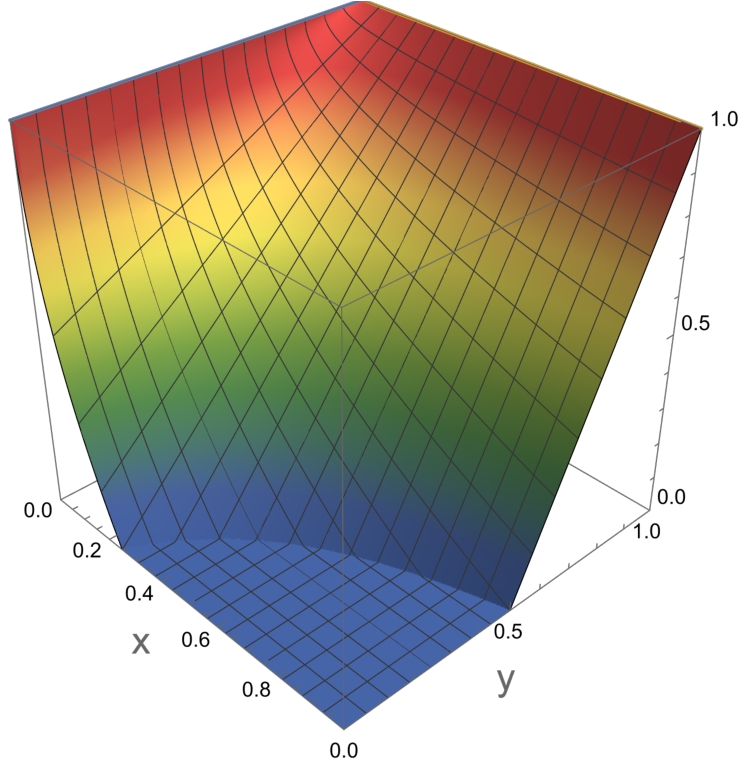
\includegraphics[width=5cm]{Ex2-1.pdf} }
		\subfloat[$I_2$]{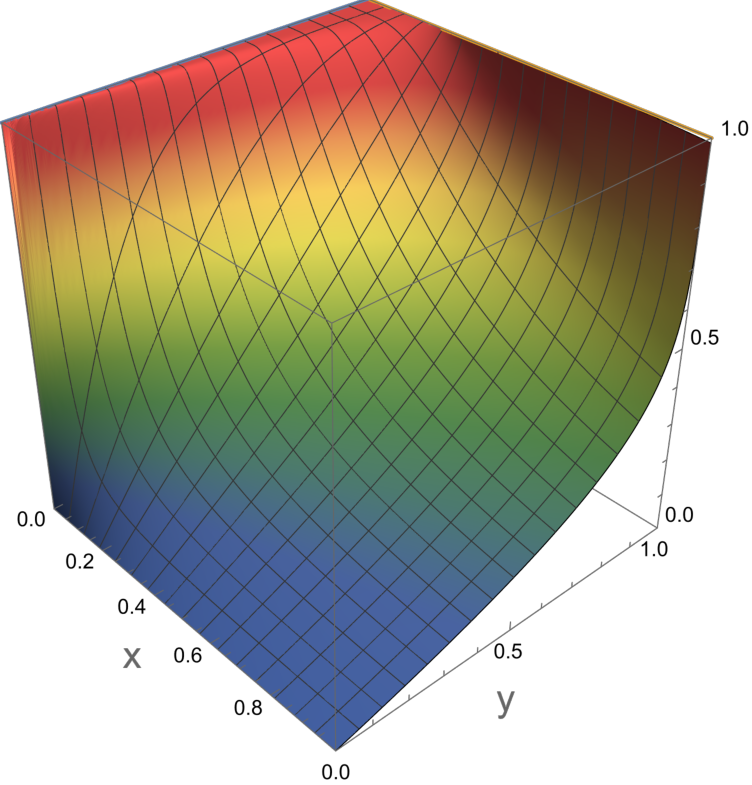
\includegraphics[width=5cm]{Ex2-2.pdf} }
		\caption[Plot of an $(f,e)$ and a $(g,e)$-implication]{Plot of fuzzy implication functions $I_{f_\lambda,e}$ and $I_{g_s,e}$ in Example \ref{example:2} with $e= \frac{1}{4}$ and $s=\lambda=2$.}\label{figure:example2}
	\end{figure}
\end{example}

At this point, we can rewrite Theorem \ref{ThmRepresentacio(h,e)} in terms of $(f,e)$ and $(g,e)$-implications using the definition of the horizontal threshold method (Theorem \ref{horizontalthreshold}) as follows.
\begin{corollary} Let $I:[0,1]^2 \to [0,1]$ be a binary function and $e \in (0,1)$. Then the following statements are equivalent:
	\begin{enumerate}[label=(\roman*)]
		\item $I$ is a generalized $(h,e)$-implication with respect to $e$, that is, $I=I^{h_g,e}$.
		\item There exists an $f$-generator and a $g$-generator with $g(1)=+\infty$ such that $I$ is given by $I=I_{I_{f,e} - I_{g,e}}$.
	\end{enumerate}
\end{corollary}

Then, in order to provide an axiomatic characterization of generalized $(h,e)$-implications based on this representation theorem, we need to study the two new families of fuzzy implication functions and provide their characterizations. Consequently, in this section we provide a further study of the properties of $(f,e)$ and $(g,e)$-implications, as particular cases of $(f,g)$ and $(g,f)$-implications. Moreover, we provide an axiomatic characterization of the two families thanks to the introduction of two new properties of fuzzy implication functions which are modifications of the standard law of importation \LI.

\subsection{Characterizations of $(f,e)$-generated implications}
In Section \ref{subsection:f-generated} we studied the additional properties of $(f,g)$-generated implications. Since $(f,e)$-generated implications are particular cases of $(f,g)$-generated implications, those results are also valid for $(f,e)$-implications. Thus, the first results of this section are corollaries which correspond to the properties of $(f,g)$-generated implications adapted to the particular case of $(f,e)$-implications. We only recall those properties that are relevant for solving the problem of the characterization of $(f,e)$-implications.

First of all, by Proposition \ref{onezonefg} we get that $(f,e)$-implications satisfy the lowest truth property, i.e., they have a trivial 1-region.

\begin{corollary}
	\label{onezone(f,e)} 
	Let $f$ be an $f$-generator and $e\in(0,1)$. Then $I_{f,e}(x,y)=1$ if and only if ($x=0$ or $y=1$).
\end{corollary}

Next, by Proposition \ref{prop:(f,g):(NP)} we recall that  $(f,e)$-generated implications do not fulfill the left neutrality principle \NP but we prove that they satisfy the modified version with $e\in(0,1)$. Observe that \NPe is also satisfied by generalized $(h,e)$-implications, strengthening the relation between the two families.

\begin{corollary} 
	Let $f$ be an $f$-generator  and $e\in(0,1)$. Then $I_{f,e}$ does not satisfy \NP, but it satisfies \NPe.
\end{corollary}
\begin{proof}
	Let be $f$ be an $f$-generator and $e \in (0,1)$. By Proposition \ref{prop:(f,g):(NP)} we obtain that $I_{f,e}$ does not satisfy \NP. On the other hand,
	$$I_{f,e}(e,x) = f^{(-1)}\left(\frac{e}{e}f(x)\right)=f^{(-1)} \circ f(x)=x, \quad \text{for all } x \in [0,1].$$
\end{proof}

Next, from Proposition \ref{negationfg} we get the expression of the natural negation of this family of fuzzy implication functions. As it will be proved later, this operator is important for characterizing $(f,e)$-implications.
\begin{corollary}
	Let $f$ be an $f$-generator and $e\in(0,1)$. The following properties hold:
	\begin{enumerate}[label=(\roman*)]
		\item If $f(0)=+\infty$, then the natural negation $N_{I_{f,e}}$ is the G\"odel or least negation $\NDOne$.
		\item If $f(0)<+\infty$, then the natural negation $N_{I_{f,e}}$ is given by
		$$N_{I_{f,e}}(x)=\left\{\begin{array}{ll} f^{-1}\left( \frac{x}{e}f(0)\right)&\hbox{if } x\leq e,\\ 0&\hbox{if } x>e.\end{array}\right.$$ 
	\end{enumerate}
	\label{negation}
\end{corollary}

Another important property of $(f,e)$-implications worthy to study is continuity, which depends on the value of the generator at zero (see Proposition \ref{prop:(f,g):continuity}).
\begin{corollary}
	\label{continuity(f,e)}
	Let $f$ be an $f$-generator  and $e\in(0,1)$. Then the following properties hold:
	\begin{enumerate}[label=(\roman*)]
		\item If $f(0)=+\infty$, then $I_{f,e}$ is continuous everywhere except at $(0,0)$.
		\item If $f(0)<+\infty$, then $I_{f,e}$ is continuous.
	\end{enumerate}
\end{corollary}

It is well known that \EP and \LI are two additional properties that are related, \LI being stronger than \EP. The following two results derived from Propositions \ref{EPfg} and \ref{prop:(f,g):(LI)} show that no $(f,e)$-implication satisfies the law of importation but, some of them satisfy the exchange principle.
\begin{corollary}
	Let $f$ be an $f$-generator and $e\in(0,1)$. Then $I_{f,e}$ satisfies \EP if and only if
	$f(0)=+\infty$.
\end{corollary}
\begin{corollary}
	Let $f$ be an $f$-generator and $e\in(0,1)$. Then $I_{f,e}$ does not satisfy \LI with any t-norm.
\end{corollary}
The last result reflects an important difference between Yager's implications and $(f,e)$-implications. It is well known that Yager's implications fulfill the law of importation \LI with respect to the product t-norm \TP. Moreover, this property plays a key role in the characterization of this family (see \cite{Massanet2012B}). Although $(f,e)$-implications do not fulfill the standard law of importation with respect to any t-norm, we prove that they satisfy two properties that resemble \LI. We provide the definition of these two new properties, which are two different modifications of the standard law of importation.

\begin{definition} 
	\label{novesli}
	A fuzzy implication function $I$ is said to satisfy
	\begin{enumerate}
		\item the \textit{$(x,ey)$-law of importation} with a t-norm $T$ for some $e \in(0,1]$, if
		$$
		I(T(x,y),z)= I(x,I(ey,z)) , \hbox{ for all } x,y,z \in [0,1].\eqno { \text{\LIey}} 
		$$
		\item the \textit{$(ex,y)$-law of importation} with a t-norm $T$ for some $e \in(0,1]$, if
		$$
		I(T(x,y),z)= I(ex,I(y,z)) , \hbox{ for all } x,y,z \in [0,1]. \eqno {\text{\LIex}}
		$$
	\end{enumerate}
\end{definition}

Notice that these two properties slightly modify the standard law of importation by limiting into $[0,e]$ the domain of one of the variables on the right-hand side of the equation. Clearly, we recover the standard law of importation when $e=1$. The motivation behind the introduction of these two properties is that we want to consider them in the characterizations of $(f,e)$-implications so they play a similar role to the one played by the standard law of importation in the characterization of Yager's implications.

The next proposition studies when the $(f,e)$-implications fulfill these two new properties. 

\begin{proposition}
	\label{LI_e(f,e)}
	Let $f$ be an $f$-generator  and $e\in(0,1)$. Then the following properties hold:
	\begin{enumerate}[label=(\roman*)]
		\item $I_{f,e}$ satisfies \LIey with respect to \TP.
		\item $I_{f,e}$ satisfies \LIex with respect to \TP if and only if $f(0)=+\infty$.
	\end{enumerate}
	\label{LIe}
\end{proposition}

\begin{proof}
	\begin{enumerate}[label=(\roman*)]
		\item On the one hand, we have
		$$I_{f,e}(xy,z)=f^{(-1)}\left(\frac{xy}{e}f(z)\right).$$
		On the other hand, we know that $f$ is strictly decreasing. Hence, for all $y,z \in [0,1]$ we get
		$$yf(z) \leq yf(0) \leq  f(0).$$
		Consequently,
		$$I_{f,e}(x,I_{f,e}(ey,z))= f^{(-1)}\left(\frac{x}{e} (f \circ f^{(-1)})(yf(z))\right) = f^{(-1)}\left(\frac{xy}{e}f(z)\right)$$
		and $I_{f,e}$ satisfies \LIey with respect to $\TP$.
		\item Let us assume that $f(0)=+\infty$. This implies that $f^{(-1)}=f^{-1}$ then, for all $x,y,z \in [0,1]$, we have
		$$I_{f,e}(ex,I_{f,e}(y,z))=f^{-1}\left(x (f\circ f^{-1})\left(\frac{y}{e}f(z)\right)\right)=f^{-1}\left(\frac{xy}{e}f(z)\right) = I_{f,e}(xy,z).$$
		Now, we assume that $f(0)< + \infty$. Consider $y,z \in [0,1]$ such that $yf(z)>ef(0)$ then we get
		$$ I_{f,e}(ex,I_{f,e}(y,z)) = f^{(-1)}\left(x (f \circ f^{(-1)})\left(\frac{y}{e}f(z)\right)\right) = f^{(-1)}(xf(0))=f^{-1}(xf(0)).$$
		Now, we can find some $x \in (0,1)$ small enough such that $xyf(z) \leq ef(0)$ and we have
		$$I_{f,e}(xy,z)=f^{(-1)}\left(\frac{xy}{e}f(z)\right) = f^{-1} \left( \frac{xy}{e}f(z)\right).$$
		Nevertheless, with the inequality $yf(z)>ef(0)$ and the strictly decreasing nature of $f^{-1}$, taking the previous considered $x \in (0,1)$ we get 
		$$ \frac{yf(z)}{e} > f(0) \Rightarrow \frac{xyf(z)}{e} > xf(0) \Rightarrow f^{-1}\left(\frac{xyf(z)}{e}\right) < f^{-1}(xf(0)).$$
		Consequently, $I_{f,e}(xy,z) \not = I_{f,e}(ex,I_{f,e}(y,z))$ and $I_{f,e}$ does not satisfy \LIex with respect to $\TP$.
	\end{enumerate}
\end{proof}

Observe that the two properties behave differently depending on the value $f(0)$. This is because of the presence of the pseudo-inverse of $f$ in the expression of these fuzzy implication functions. This fact results in the need to consider two different cases to provide the characterization of $(f,e)$-implication.


At this stage, using the preceding results we can present the characterization of $(f,e)$-generated implications with $f(0)<+\infty$.

\begin{theorem}\label{caractf0fin}
	Let $I:[0,1]^2\to [0,1]$ be a binary function and $e\in(0,1)$. Then the following statements are equivalent:
	\begin{enumerate}
		\item[(i)] $I$ is an $(f,e)$-generated implication with $f(0)<+\infty$.
		\item[(ii)] $I$ satisfies \LIey with $\TP$ and $N_I$ is a continuous fuzzy negation which is strictly decreasing in $(0,e)$ and such that $N_I(e)=0$.
	\end{enumerate}
	Moreover, in this case the $f$-generator is given by 
	\begin{equation}f(x)=N_{I}^{(-1)}(x)=\left\{\begin{array}{ll} N_I^{-1}(x)&\hbox{if } x >0,\\ e&\hbox{if } x=0.\end{array}\right.
		\label{GenFinites}
	\end{equation}
\end{theorem}

\begin{proof}
	Let $I$ be a binary function with $N_I$ a continuous fuzzy negation which is strictly decreasing in $(0,e)$ for some $e \in (0,1)$ such that $N_I(e)=0$ and satisfying \LIey with $\TP$. Let us define $f(x)=N_{I}^{(-1)}(x)$. First of all, we prove Equation (\ref{GenFinites}). Let us recall the definition of the pseudoinverse of a function
	$$N_I^{(-1)}(x) = \sup\{ z \in [0,1] ~,~ N_I(z)>x \}.$$
	Then, if $x=0$ we have
	$$N_I^{(-1)}(0)=\sup \{ z \in [0,1] ~,~ N_I(z)>0 \}=e.$$
	Otherwise, if $x>0$ as we know that $N_I$ is a bijection in $[0,e]$ and takes all the values in $[0,1]$ we obtain
	$$ N_I^{(-1)}(x)= \sup \{ z \in [0,1] ~|~ z < N_I^{-1}(x) \}=N_I^{-1}(x).$$
	Now, we see that $f$ is an $f$-generator. Since $N_I$ is a bijection in $[0,e]$ with $N_I(e)=0$, $f$ is continuous. Also, as $N_I$ is a strictly decreasing function in $[0,e]$, $f$ is strictly decreasing in $[0,1]$. In addition $f(0)=e < + \infty$ and $f(1)=N_I^{-1}(1)=0$. Now, we have
	$$ f^{-1}(x)= \left\{\begin{array}{ll} f^{-1}(x)&\hbox{if } x \in [0,f(0)],\\ 0&\hbox{if } x \in (f(0),1] ,\end{array}\right. = 
	\left\{\begin{array}{ll} N_I(x)&\hbox{if } x \in [0,e],\\ 0&\hbox{if } x \in (e,1] ,\end{array}\right.
	$$
	and then $f^{(-1)}(x)=N_I(x)$ for all $x \in [0,1]$. Finally, let us see that $I=I_{f,e}$. First, we develop the expression of $I_{f,e}$ with respect to the chosen $f$-generator. Using that $I$ satisfies \LIey with $\TP$ we get
	\begin{eqnarray*}
		I_{f,e}(x,N_I(y))&=&f^{(-1)}\left(\frac{x}{e}(f\circ f^{(-1)})(y)\right) =N_I\left(\frac{x}{e}(N_I^{(-1)} \circ N_I)(y)\right)\\
		&=& \left\{\begin{array}{ll} N_I\left(\frac{xy}{e}\right)&\hbox{if } N_I(y)>0,\\ N_I(x)&\hbox{if }N_I(y)=0 ,\end{array}\right. = \left\{\begin{array}{ll} 	I \left(\frac{xy}{e},0\right)&\hbox{if } y \in [0,e) ,\\ I(x,0) &\hbox{if }y\in [e,1] ,\end{array}\right. \\ 
		&=& \left\{\begin{array}{ll} 	I(x,I(y,0))&\hbox{if } y \in [0,e) ,\\ I(x,0) &\hbox{if }y\in [e,1] ,\end{array}\right. =
		\left\{\begin{array}{ll} 	I(x,N_I(y)) &\hbox{if } y \in [0,e) ,\\ I(x,N_I(y)) &\hbox{if }y\in [e,1] ,\end{array}\right.
	\end{eqnarray*}
	and we have that $ I_{f,e}(x,N_I(y)) = I(x,N_I(y))$ for all $y \in [0,1]$. Now, since $N_I$ takes all the values in $[0,1]$, the result follows.
	The reciprocal is guaranteed by (i)-Proposition \ref{LIe} and (ii)-Corollary \ref{negation}.
\end{proof}
\begin{remark} In order to show that the two properties considered in (ii)-Theorem \ref{caractf0fin} are independent from each other we provide the following two examples of fuzzy implication functions:
	$$I_1(x,y)= \left\{\begin{array}{ll} y^{2x}& \hbox{if } x>0 \hbox{ or } y>0,\\ 1&\hbox{if } x=0 \hbox{ and } y=0,\end{array}\right. \quad I_2(x,y)= \left\{\begin{array}{ll} 1-2x(1-y)& \hbox{if } x \in [0,0.5],\\ y&\hbox{if } x \in (0.5,1].\end{array}\right.$$
	If we consider $e=0.5$ it is easy to prove that $I_1$ satisfies \LIey with respect to $\TP$ but $N_{I_1}=\NDOne$ is not continuous. On the other hand, the natural negation of $I_2$ is the following
	$$N_{I_2}(x)=\left\{\begin{array}{ll} 1-2x& \hbox{if } x \in [0,0.5],\\ 0&\hbox{if } x \in (0.5,1].\end{array}\right.$$
	Thus, $N_{I_2}$ is continuous, strictly decreasing on $x \in [0,0.5]$ and $N_{I_2}(0.5)=0$ but $I_2$ does not satisfy \LIey with respect to $\TP$ since for $x=0.75$, $y=0.5$ and $z=0.5$ we have that
	$$I_2(\TP(0.75,0.5),0.5)=I_2(0.75 \cdot 0.5, 0.5)=0.625 < 0.75 =I_2(0.75, I_2(0.5 \cdot 0.5,0.5)).$$
\end{remark}

From this point on, we focus our attention to the case $f(0)=+\infty$. For providing the characterization of the remaining subfamily, we need to consider some other properties. First of all, we study the monotonicity of the horizontal and vertical sections of $(f,e)$-implications with  $f(0)=+\infty$.


\begin{lemma}\label{lema-previ}
	Let $f$ be an $f$-generator with $f(0)=+\infty$ and $e\in(0,1)$. Then the following properties hold:
	\begin{enumerate}[label=(\roman*)]
		\item The horizontal sections of $I_{f,e}$, $h_k(x)=I_{f,e}(x,k)$, are strictly decreasing for all $x\in[0,1]$ and $k\in(0,1)$.
		\item The vertical sections of $I_{f,e}$, $v_k(x)=I_{f,e}(k,x)$, are strictly increasing for all $x\in[0,1]$ and $k\in(0,1]$.
	\end{enumerate}
\end{lemma}

\begin{proof}
	\begin{enumerate}[label=(\roman*)]
		\item Let us assume $x_1,x_2\in [0,1]$ such that $x_1 < x_2$, then $\frac{x_1}{e}f(k) < \frac{x_2}{e}f(k)$. Now, since $f$ is strictly decreasing, $f^{-1}$ is also strictly decreasing and we get
		$$h_k(x_1)=I_{f,e}(x_1,k)=f^{-1}\left(\frac{x_1}{e} f(k)\right) > f^{-1} \left(\frac{x_2}{e}f(k)\right) = I_{f,e}(x_2,k)=h_k(x_2).$$
		
		Thus, the horizontal sections of $I_{f,e}$ are strictly decreasing for all $x \in [0,1]$ and $k\in (0,1)$.
		\item Let us assume $x_1,x_2 \in [0,1]$ such that $x_1<x_2$ then, since $f$ is strictly decreasing, we get that $\frac{k}{e}f(x_1) > \frac{k}{e}f(x_2)$ . Now because $f^{-1}$ is strictly decreasing we have
		$$v_k(x_1)=I_{f,e}(k,x_1)=f^{-1}\left(\frac{k}{e}f(x_1)\right) < f^{-1}\left(\frac{k}{e}f(x_2)\right) = I_{f,e}(k,x_2)=v_k(x_2)$$
		\noindent and the vertical sections of $I_{f,e}$ are strictly increasing for all $x\in [0,1]$ and $k \in (0,1]$.
	\end{enumerate}
\end{proof}


Before presenting the characterization of $(f,e)$-implications with $f(0)=+\infty$ we give some preliminary results. The following proposition emphasizes that the two new properties \LIey and \LIex with respect to $\TP$, in conjunction with the property that the binary operation equals $1$ if and only if ($x=0$ or $y=1$), and the continuity except at $(0,0)$, are crucial since they ensure that many other properties hold.

\begin{lemma}\label{lema-previ2} 
	Let $e\in(0,1)$ and $I:[0,1]^2\to [0,1]$ be a continuous function everywhere except at $(0,0)$ satisfying \LIey and \LIex with respect to $\TP$ and ($I(x,y)=1\Leftrightarrow x=0$ or $y=1$). Then the following properties hold:
	\begin{enumerate}[label=(\roman*)]
		\item $I(e,0)=0$.
		\item $I$ satisfies \NPe.
		\item The horizontal sections of $I$, $h_k:[0,1]\to[0,1]$ given by $h_k(x)=I(x,k)$, are strictly decreasing for all $k\in(0,1)$.
		\item $N_I=\NDOne$.
		\item The vertical sections of $I$, $v_k:[0,1]\to[0,1]$ given by $v_k(x)=I(k,x)$, are strictly increasing for all $k\in(0,1]$.
	\end{enumerate}
\end{lemma}

\begin{proof}
	\begin{enumerate}[label=(\roman*)]
		\item First of all we are going to prove that $I(e,0)=0$. On the contrary, let us suppose that $I(e,0)=a>0$ and let us get a contradiction.
		By \LIey for all $x \in [0,1]$ we get
		$$I(x,a)=I(x,I(e,0))=I(\TP(x,1),0)=I(x,0),$$
		and $N_I(x)=h_0(x)=h_a(x)$ is continuous since $h_a$ is. Now, since $I$ is continuous except at $(0,0)$ we get that all the horizontal sections of $I$ are continuous.\\
		Let us prove that the horizontal sections $h_k(x)$ are decreasing for all $k \in [0,1]$. For $k=1$ it is obvious since $h_1(x)=1$ for $x\in [0,1]$.  Otherwise, consider $x_1,x_2 \in [0,1]$ such that $x_1<x_2$ with $h_k(x_1)=h_k(x_2)$. If $h_k(x_1)=h_k(x_2)=1$ then $x_1=x_2=0$ and we get a contradiction. Then, let us assume $h_k(x_1)=h_k(x_2)<1$ with $0<x_1<x_2$ and by \LIex we get
		$$ I \left( \frac{ex_1}{x_2},h_k(x_2) \right) = I\left( \frac{ex_1}{x_2},I(x_2,k)\right) = I(x_1,k)=h_k(x_1)=h_k(x_2).$$
		Similarly, we obtain
		\begin{eqnarray*}
		 h_k(x_2) &=& I \left(\frac{ex_1}{x_2},h_k(x_2)\right) = I \left( \frac{ex_1}{x_2}, I\left( \frac{ex_1}{x_2},h_k(x_2)\right)\right) = I \left( e \left(\frac{x_1}{x_2}\right)^2,h_k(x_2) \right) \\
		 &=& I \left( e \left( \frac{x_1}{x_2}\right)^2, I(x_2,k)\right).
		 \end{eqnarray*}
		Consequently, if we iterate this process we obtain
		$$ I\left( e \left(\frac{x_1}{x_2}\right)^n , h_k(x_2)\right) = h_k(x_2),$$
		for all $n>0$. Now, if $h_k(x_2)=0$ we have
		$$ I \left( e \left(\frac{x_1}{x_2}\right)^n,a\right) = I \left( e \left(\frac{x_1}{x_2}\right)^n,0\right) =h_k(x_2)=0$$
		which is a contradiction since
		$$ \lim_{n\to+\infty}  I \left( e \left(\frac{x_1}{x_2}\right)^n,a\right) = I(0,a)=1>0.$$
		On the other hand, if $h_k(x_2)>0$ we have
		$$ h_k(x_2)=\lim_{n\to+\infty}  I \left( e \left(\frac{x_1}{x_2}\right)^n,h_k(x_2)\right) = I(0, h_k(x_2))=1 >h_k(x_2),$$
		and we also obtain a contradiction. Hence $h_k$ is injective and since $h_k(0)=I(0,k)=1$ we get that $h_k$ is decreasing and continuous for all $k \in [0,1]$. Besides, we also have that all the vertical sections are continuous since $v_0(x)= I(0,x)=1$ for all $x \in [0,1]$. Consequently, we get that $I$ is monotonic with respect to the first variable and continuous in each variable. Now by Theorem \ref{theorem:A04} we have that $I$ is, in fact, continuous so we get a contradiction.
		\item Consider $y \in (0,1)$. Since $v_e(x)$ is continuous with $v_{e}(0)=I(e,0)=0$ and $v_e(1)=1$ then there exists a $z\in (0,1)$ such that $v_e(z)=y$. Now, by \LIex we get
		$$I(e,y)=I(e,v_e(z))=I(e,I(e,z))=I(e,z)=v_e(z)=y.$$
		Also, $I(e,0)=0$ and $I(e,1)=1$. So $I$ satisfies \NPe.
		\item Consider $k \in (0,1)$ and let us prove that $h_k$ is injective considering three cases:
		\begin{itemize}
			\item  If $h_k(x_1)=h_k(x_2)=1$ then $x_1=x_2=0$.
			\item  If $0<h_k(x_1)=h_k(x_2)<1$ then necessarily $x_1,x_2>0$. Let us assume $x_1<x_2$,  by \LIex we get
			$$I \left( e\frac{x_1}{x_2}, h_k(x_2) \right) = I \left( e\frac{x_1}{x_2}, I(x_2,k) \right) = I(x_1,k)=h_k(x_1)=h_k(x_2).$$
			Consequently,
			$$ h_k(x_2) = I \left( e \frac{x_1}{x_2},h_k(x_2)\right) = I \left( e \frac{x_1}{x_2}, I \left( e \frac{x_1}{x_2}, h_k(x_2) \right) \right) = I \left( e \left(\frac{x_1}{x_2}\right)^2,h_k(x_2)\right).$$
			Following this idea we get
			$$I \left( e \left( \frac{x_1}{x_2}\right)^n,h_k(x_2) \right) = h_k(x_2),$$
			for all $n>0$. Since we have
			$$ h_k(x_2) = \lim_{n \to +\infty} I \left( e \left( \frac{x_1}{x_2}\right)^n,h_k(x_2)\right)=I(0,h_k(x_2))=1>h_k(x_2),$$
			we get a contradiction.
			\item  If $h_k(x_1)=h_k(x_2)=0$, let us assume $0 < x_1 \leq x_2$. We need to distinguish between two cases:
			\begin{itemize}
				\item  If $e> x_1$, since $h_k$ is continuous and $h_k(0)=I(0,k)=1$, there exists $x' \in (0,x_1)$ and $x^{*}\in(0,k)$ such that $h_k(x')=x^{*}$. Now, by (ii) we get that $h_k(e)=I(e,k)=k$ and there exists $x'' \in (x_1,e)$ with $h_k(x'')=x^{*}$ obtaining a contradiction as in the previous case. 
				\item  If $e \leq x_1 <x_2 \leq 1$ by \LIex we get that
				$$h_k(ex_1)=I(ex_1,k)=I(e^2,I(x_1,k))=I(e^2,h_k(x_1))=I(e^2,0),$$
				$$h_k(ex_2)=I(ex_2,k)=I(e^2,I(x_2,k))=I(e^2,h_k(x_2))=I(e^2,0),$$
				then $h_k(ex_1)=h_k(ex_2)<1$ with $ex_1 \leq ex_2 \leq e$. Now, if $h_k(ex_1)=h_k(ex_2)=0$ we get a contradiction as we have seen before and if $h_k(ex_1)=h_k(ex_2)>0$ then necessarily by a previous case $ex_1=ex_2$ and we get that $x_1=x_2$.
			\end{itemize}
		\end{itemize}
		Hence $h_k$ is injective and since $h_k(0)=I(0,k)=1$ we get that $h_k$ is strictly decreasing for all $k \in (0,1)$.
		\item First of all, let us see that $h_0(x)$ is decreasing for $x \in [0,1]$. Consider $0<x_1<x_2$ and a sequence $\{y_n\}_{n \geq 0}$ such that $y_n\in(0,1)$ and $y_n \rightarrow 0$. Then, using Point (iii) we get that
		$$h_{y_n}(x_1)=I(x_1,y_n)>I(x_2,y_n)=h_{y_n}(x_2),$$
		for all $n>0$. Then,
		$$I(x_1,0)=\lim_{n \to +\infty}I(x_1,y_n) \geq \lim_{n \to +\infty} I(x_2,y_n)=I(x_2,0).$$
		Now, we want to prove that $N_I=\NDOne$. We will see that $I(x,0)=0$ for all $x>0$. Let us assume that there exists $x_0>0$ such that $I(x_0,0)=a>0$. Then, for all $x\in(0,1)$, the sequence $\{x^n\}_{n \geq 0}$ is such that $x^n \to 0$ and by \LIex we have that
		$$ I(ex,a)=I(ex,I(x_0,0))=I(xx_0,0),$$
		$$I(ex^2,a)=I(ex,I(ex,a))=I(ex,I(xx_0,0))=I(x^2x_0,0).$$
		Consequently, for all $n>0$ we have that
		$$I(ex^n,a)=I(x^n x_0,0).$$
		Now, taking limits we get
		\begin{equation}
			\lim_{n \to +\infty} I(x^nx_0,0)=I(0,a)=1.
			\label{1}
		\end{equation}
		We will see that in this case we get a contradiction with the non-continuity of $I$ at the point $(0,0)$. Let $\{x_n\}_{n \geq 0}$ be a sequence such that $x_n>0$ and $x_n \to 0$ and $\varepsilon > 0$. By Equation (\ref{1}) there exists $n_0 \in \mathbb{N}$ such that for all $n \geq n_0$ we have that
		$$ I(x^{n}x_0,0)>1-\varepsilon.$$
		For this $n_0$ we have $x^{n_0}x_0>0$, and since $x_n \to 0$ there exists $n_1 \in \mathbb{N}$ such that $x_n \leq x^{n_0}x_0$ for all $n \geq n_1$. Then
		$$I(x_n,0) \geq I(x^{n_0}x_0,0) > 1-\varepsilon$$
		for all $n \geq n_1$. Now, we get that the sequence $\{I(x_n,0)\}_{n \geq 0}$ converges to 1 and we have that $h_0(x)$ is continuous in $x \in [0,1]$. Thus, we have a contradiction by the same argument used in Point (i). Hence, $N_I=\NDOne$.
		\item Consider $y_1 \leq y_2$ and $k \in (0,1)$ such that $v_k(y_1)=v_k(y_2)$, we will see that necessarily $y_1=y_2$ distinguishing three cases:
		\begin{itemize}
			\item  If $v_k(y_1)=v_k(y_2)=1$ then $y_1=y_2=1$.
			\item  If $v_k(y_1)=v_k(y_2)=0$ and $y_1=0$, $y_2>0$ we have two more cases:
			\begin{itemize}
				\item  If $k \in (e,1)$ then by Points (ii) and (iii) we get  $$v_k(y_1)=I(k,y_1) < I(e,y_1) =y_1=0$$
				which is a contradiction since the range of $v_k$ is $[0,1]$.
				\item  If $k \in (0,e]$ then again by Points (ii) and (iii) we have
				$$0=v_k(y_2)=I(k,y_2) \geq I(e,y_2)=y_2.$$
				Contradiction with the assumption $y_2>0$.
			\end{itemize}
			\item  If $0 \leq v_k(y_1)=v_k(y_2)<1$ and $0<y_1 \leq y_2$ then there exists an $x^{*} \in (0,1)$ such that $x^{*}<y_1 \leq y_2$ and we have that
			$$h_{x^{*}}(0)=I(0,x^{*})=1 ~,~ h_{x^{*}}(e)=I(e,x^{*})=x^{*}.$$
			Since the horizontal sections $h_k$ are continuous, there exist $x_1,x_2 \in (0,e)$ such that
			$$h_{x^*}(x_1)=I(x_1,x^{*})=y_1 ~,~ h_{x^*}(x_2)=I(x_2,x^{*})=y_2.$$
			Then, by \LIey we get
			\begin{eqnarray*}
			I\left(\frac{kx_1}{e},x^{*}\right) &=& I(k,I(x_1,x^{*}))=I(k,y_1) = I(k,y_2) \\
			&=& I(k,I(x_2,x^{*}))=I\left(\frac{kx_2}{e},x^{*}\right).
			\end{eqnarray*}
			Now, since the section $h_{x^*}$ is injective we get that
			$$\frac{kx_1}{e}=\frac{kx_2}{e} \Rightarrow x_1=x_2 \Rightarrow y_1=y_2.$$
		\end{itemize}
		Hence, the vertical sections $v_k$ are injective for $k \in (0,1)$. Now, since $v_k(1)=I(k,1)=1$ we get that $v_k$ are, in fact, strictly increasing for all $k \in (0,1)$.
	\end{enumerate}
\end{proof}

Observe that the above proposition uses the two variations of the law of importation. We remark that the property \LIex with respect to $\TP$ is not satisfied by $(f,e)$-generated implications with $f(0)<+\infty$, but it plays a capital role in the characterization of $(f,e)$-generated implications with $f(0)=+\infty$.

Lastly, we present the characterization of $(f,e)$-generated implications with $f(0)=+\infty$.

\begin{theorem}\label{caractf0inf}
	Let $I:[0,1]^2\to [0,1]$ be a binary function and $e\in(0,1)$. Then the following statements are equivalent:
	\begin{enumerate}
		\item[(i)] $I$ is an $(f,e)$-generated implication with $f(0)=+\infty$.
		\item[(ii)] $I$ satisfies \LIey and \LIex with respect to $\TP$, $I$ is continuous except at $(0,0)$ and ($I(x,y)=1 \Leftrightarrow x=0 \hbox{ or } y=1$). 
		\item[(iii)] $I$ satisfies \LIey and \LIex with respect to $\TP$, $N_I=\NDOne$, $I$ is continuous except at $(0,0)$ and there exists $k_0\in(0,1)$ such that 
		\begin{itemize}
			\item $h_k$ is strictly decreasing with $h_k(0)=1$ and $h_k(e)=k$ for all $k\in(0,k_0]$,
			\item $v_k$ are strictly increasing on the interval $[0,k_0]$ for all $k\in(0,1)$.
		\end{itemize}
		\item[(iv)] $I$ satisfies \LIey and \LIex with respect to $\TP$, $N_I=\NDOne$ and there exists $k\in(0,1)$ such that 
		\begin{itemize}
			\item $h_k$ is continuous and strictly decreasing with $h_k(0)=1$ and $h_k(e)=k$,
			\item $h_{\bullet}^{-1}(k):(0,k)\to[0,e]$ that assigns $h_y^{-1}(k)$ to some $y\in(0,k)$, is a well-defined, continuous and strictly increasing function satisfying 
			$\displaystyle \lim_{y\to 0^+}{h_y^{-1}(k)}=0$. 
		\end{itemize}
	\end{enumerate}
	Moreover, in this case the $f$-generator is given by
	\begin{equation}
		\label{fgen}
		f(x)=\left\{\begin{array}{ccl} \dfrac{h_k^{-1}(x)}{e} &\hbox{if }& k\leq x \leq 1,\\[1em] \dfrac{e}{h_x^{-1}(k)}&\hbox{if }& 0<x<k,\\[1em] +\infty &\hbox{if }& x=0.\end{array}\right.
	\end{equation}
\end{theorem}
\begin{proof}
	First, {\bf (i)$\Rightarrow$(ii)} is straightforward by Corollaries \ref{onezone(f,e)} and \ref{continuity(f,e)}  and Proposition \ref{LI_e(f,e)}.\\
	In order to prove that {\bf (ii)$\Rightarrow$(iii)} it is enough to use Lemma \ref{lema-previ2}.\\
	Let us prove {\bf(iii)$\Rightarrow$(iv)}. Consider $k=k_0$ then $h_k$ is continuous and strictly decreasing because $h_{k_0}$ is. Furthermore,
	$$h_k(0)=h_{k_0}(0)=1 ~,~ h_k(e)=h_{k_0}(e)=k=k_0.$$
	\begin{itemize}
		\item Let us prove that $h_{\bullet}^{-1}(k)$ is a well-defined function. Consider $y \in (0,k)$ then $h_y : [0,1] \to [h_y(1),1]$. Notice that $k\in [h_y(1),1]$ because we have that $h_y(0)=1$ and $h_y(e)=y$. Since $h_y$ is continuous and strictly decreasing there exists a unique $x_0 \in (0,1)$ such that $h_y(x_0)=I(x_0,y)=k$, then $h_y^{-1}(k)=x_0$.
		\item We will see that $h_{\bullet}^{-1}(k)$ is strictly increasing. Consider $0<y_1<y_2<k$, $x_1=h_{y_1}^{-1}(k)$ and $x_2=h_{y_2}^{-1}(k)$. Then by the fact that the vertical sections $v_{k'}$ are strictly increasing in $[0,k]$ for all $k' \in (0,1)$ we get that
		$$k=I(x_1,y_1)<I(x_1,y_2).$$
		Since $h_{y_2}$ is strictly decreasing we obtain that
		$$h_{y_2}(x_1)=I(x_1,y_2)>k = I(x_2,y_2)=h_{y_2}(x_2) \Rightarrow x_1 < x_2 \Rightarrow h_{y_1}^{-1}(k) < h_{y_2}^{-1}(k).$$
		\item Now, we prove that $h^{-1}_{\bullet}$ is continuous. Consider a decreasing sequence $\{y_n\}_{n \geq 0}$ with limit $y \in (0,k)$. We will see that the sequence $\{h^{-1}_{y_n}(k)\}_{n \geq 0}$ converges to $h_{y}^{-1}(k)$. Denote $x_n=h^{-1}_{y_n}(k)$ for all $n$ and let $x'$ be the limit of  $\{x_n\}_{n \geq 0}$, we know that this limit exists since $\{x_n\}_{n \geq 0}$ is bounded and strictly increasing. Now, since $I$ is continuous except at $(0,0)$ then $\{I(x_n,y_n)\}_{ n \geq 0}$ converges to $I(x',y)$. On the other hand, $I(x_n,y_n)=k$ for all $n$, then $I(x',y)=k$ and we get that $x' = h_y^{-1}(k)$. Therefore,
		$$\lim_{y_n \to y^{+}} h_{y_n}^{-1}(k)=h_y^{-1}(k).$$
		A similar argument taking an increasing sequence $\{y_n\}_{n \geq 0}$ such that $y_n \to y$ shows that
		$$ \lim_{y_n \to y^{-}} h_{y_n}^{-1}(k) =h_y^{-1}(k).$$
		Thus $h_y^{-1}(k)$ is continuous.
		\item Finally, we see that $\displaystyle \lim_{y \to 0^{+}} h_y^{-1}(k)=0$ for all $x \in [0,1]$ and $y \in (0,k)$. Consider a decreasing sequence $\{y_n\}_{n \geq 0}$ with $y_n \in (0,1)$ and $y_n \to 0$. Let $x'$ be the limit of $\{h_{y_n}^{-1}(k)\}_{n \geq 0}$. Let us assume that $x' \not = 0$, then $\{ I(h_{y_n}^{-1}(k),y_n) \}_{n \geq 0}$ converges to $I(x',0) = \NDOne(x)=0$. But we also have that $I(h^{-1}_{y_n}(k),y_n)=k$ for all $n>0$ and we get a contradiction.
	\end{itemize}
	Finally, let us prove that {\bf (iv)$\Rightarrow$(i)}. Consider the function $f$ given by Equation (\ref{fgen}) and let us prove that is an $f$-generator.
	\begin{itemize}
		\item Firstly, we will prove that $f$ is continuous and strictly decreasing. We see that $\frac{h_k^{-1}}{e}$ is continuous and strictly decreasing on the interval $[k,1]$ since $h_k$ is a continuous and strictly decreasing function. In addition $\frac{e}{h_{\bullet}^{-1}(k)}$ is also continuous and strictly decreasing since $h_x^{-1}(k) \not = 0$ for all $x \in (0,k)$ and $h_{\bullet}^{-1}(k)$ is strictly increasing. Finally, in order to see the continuity at $x=k$ we have that $ f(k)=\frac{h_k^{-1}(k)}{e}=\frac{e}{e}=1$ and
		$$\lim_{x \to k^{+}}f(x)=\lim_{x \to k } \frac{h_k^{-1}(x)}{e}= \frac{h_k^{-1}(k)}{e}=1,$$
		$$\lim_{x \to k^{-}}f(x)=\lim_{x \to k } \frac{e}{h_x^{-1}(k)}= \frac{e}{h_k^{-1}(k)}=1.$$
		\item $f(0)=+\infty$ by construction and $f(1)=\frac{h_k^{-1}(1)}{e}=0.$
	\end{itemize}
	Finally, we will prove that $I_{f,e}(x,y)=I(x,y)$ considering different cases:
	\begin{itemize}
		\item If $x \in [0,1]$ with $y \in [k,1]$ then there exists $z \in [0,e]$ such that $y=h_k(z)$ and we have
		$$I_{f,e}(x,y)=f^{-1}\left(\frac{x}{e}f(y)\right) = f^{-1} \left(\frac{x}{e}f(h_k(z))\right).$$
		Since $h_k(z) \in [h_k(e),h_k(0)]=[k,1]$ then we get
		$$I_{f,e}(x,y)=f^{-1}\left(\frac{xz}{e^2}\right).$$
		Now, we distinguish two subcases:
		\begin{itemize}
			\item If $xz \leq e^2$ then since $f^{-1}(w)=h_k(ew)$ for all $0 \leq w \leq 1$ and by \LIey we get
			$$ I_{f,e}(x,y) =h_k\left(\frac{xz}{e}\right) = I\left( \frac{xz}{e},k \right) = I(x,I(z,k))=I(x,y).$$
			\item If $xz > e^2$ then $f^{-1}\left(\frac{xz}{e^2}\right)=x'$ with $I\left(\frac{e^3}{xz},x'\right)=k$ . By \LIex, we get that
			$$I\left(\frac{e^3}{xz},I(x,y)\right)=I\left(\frac{e^2}{z},y\right) = I \left(\frac{e^2}{z},h_k(z)\right) = I\left(\frac{e^2}{z},I(z,k)\right)=I(e,k)=k.$$
			Now, since $h_{\bullet}^{-1}$ is strictly increasing we get
			$$I(x,y)=x'=I_{f,e}(x,y).$$
		\end{itemize}
		\item If $x \in [0,1]$ and $ y \in (0,k)$ we have
		$$I_{f,e}(x,y)=f^{-1}\left(\frac{x}{e}f(y)\right)=f^{-1}\left(\frac{x}{h_y^{-1}(k)}\right).$$
		Now, let us consider two more cases:
		\begin{itemize}
			\item If $ x \leq h_y^{-1}(k)$ then by \LIex we obtain that
			$$I_{f,e}(x,y)=h_k\left(\frac{ex}{h_y^{-1}(k)}\right) = I\left(\frac{ex}{h_y^{-1}(k)},k\right) = I\left(\frac{ex}{h_y^{-1}(k)}, I(h_y^{-1}(k),y)\right)=I(x,y).$$
			\item If $x> h_y^{-1}(k)$  then $f^{-1}\left(\frac{x}{h_y^{-1}(k)}\right)=x'$ such that $I\left(\frac{eh_y^{-1}(k)}{x},x'\right)=k$. Now, again by \LIex we have
			$$I \left(\frac{eh_y^{-1}(k)}{x},I(x,y)\right) = I(h_y^{-1}(k),y)=k,$$
			and again since $h_{\bullet}^{-1}$ is strictly increasing we  get that
			$$I(x,y)=x'=I_{f,e}(x,y).$$
		\end{itemize}
		\item Finally, if $x \in [0,1]$ and $y=0$ we have
		\begin{eqnarray*}
		I_{f,e}(x,0)&=&f^{-1}\left( \frac{x}{e} \cdot (+ \infty) \right)= \left\{ \begin{array}{ll}
			f^{-1}(0 \cdot (+\infty))=f^{-1}(0)=1 &   \text{if }   x=0, \\
			\\ f^{-1}\left(\frac{x}{e} \cdot (+\infty)\right)= f^{-1}(+\infty)=0 &\text{if } x>0,
		\end{array} \right. \\
		&=&\NDOne(x)=I(x,0).
		\end{eqnarray*} 
	\end{itemize}
\end{proof}
\begin{remark}\label{rmk2f}
	Recall that by Lemma \ref{lema-previ}, the horizontal sections $h_k$ and the vertical sections $v_k$ of an $(f,e)$-generated implication with $f(0)=+\infty$ are continuous and strictly decreasing or increasing, respectively, for all $k\in(0,1)$. Thus in fact any $k\in(0,1)$ can be used in order to obtain the $f$-generator through Equation (\ref{fgen}). 
\end{remark}

Notice that the previous characterization follows a similar structure to the one presented in \cite{Massanet2012B} for Yager's $f$-generated implications with $f(0)=+\infty$ using, in this case, the two modified laws of importation introduced in Definition \ref{novesli}.

In Table \ref{independence} we give some examples of functions $I:[0,1]^2\to[0,1]$ showing that none of the properties considered in (ii)-Theorem \ref{caractf0inf} is stronger than any of the others. More precisely, these examples show that none of the four properties in (ii)-Theorem \ref{caractf0inf}  can be directly deduced from one of the other properties. Perhaps the most remarkable result is that there exist binary operations in the unit interval which satisfy \LIex but do not satisfy \LIey and vice-versa. Note that these examples are not enough to ensure the independence of the four properties, to do such statement we should find binary operations which satisfy three of the properties and do not satisfy the excluding property, for each combination of cases. However, since \LIex and \LIey are two new properties in the literature, it is a difficult task to find such examples and a deeper study is needed. For instance, finding the function in the second row of Table \ref{independence} which satisfies \LIex but does not satisfy \LIey has been a challenging problem.

\begin{table}[t]
	\begin{center}
		\setlength\tabcolsep{7pt}
		\renewcommand{\arraystretch}{1.75} \large
		\begin{adjustbox}{max width=\textwidth}
			\begin{tabular}{|p{57mm}|M{30mm}|M{30mm}|M{30mm}|c|c|} \hline
				\centering \bf Function $I$  & \bf Fuzzy Impl. Funct.  & \LIey with $\TP$ for some $e \in (0,1)$ &\LIex with $\TP$ for some $e \in (0,1)$ &  \bf { $I(x,y)=1\Leftrightarrow$  $x=0$ or $y=1$} & \bf $I$ cont $\setminus\{(0,0)\}$ \\
				\hline
				$\left\{\begin{array}{ll} \dfrac{xy}{e}& \hbox{if } xy\leq e,\\ 1&\hbox{if } xy>e.\end{array}\right.$& \xmark & \cmark & \xmark & \xmark & \xmark\\
				\hline
				$\left\{ \begin{array}{ll}
					y^{\frac{x}{e}}  & \hbox{if }    x\ln(y) < -0.5e,\\
					1 &   \hbox{if }  x\ln(y) \geq -0.5e.
					
				\end{array}
				\right.$ & \cmark &\xmark & \cmark & \xmark & \xmark\\ \hline
				$\max\{1-x,y\}$ & \cmark &\xmark & \xmark & \cmark & \xmark\\ \hline
				$\left\{\begin{array}{ll} \dfrac{xy}{x^2+y^2}& \hbox{if } x,y>0,\\ 0&\hbox{if } x=y=0.\end{array}\right.$& \xmark &\xmark & \xmark & \xmark &\cmark \\ \hline
				$\left\{\begin{array}{ll} y^{x(1-y)}& \hbox{if } x>0 \hbox{ or } y>0,\\ 
					1&\hbox{if } x=y=0.\end{array}\right.$& \cmark &\xmark & \xmark & \cmark & \cmark \\ 
				\hline      
				$\left\{ \begin{array}{ll}
					1-\frac{x}{e} + \frac{xy}{e} &   \hbox{if }   y \geq 1-\frac{e}{x}, \\ 0  & \hbox{if }   y < 1-\frac{e}{x}.
				\end{array}
				\right.$ & \cmark &\cmark & \xmark & \cmark & \xmark\\ \hline
				
				$\left\{\begin{array}{ll} 1& \hbox{if } x=0 \hbox{ or } y=1 ,\\ 0& \hbox{otherwise}.\end{array}\right.$& \cmark &\cmark & \cmark & \cmark & \xmark\\ 
				\hline
				$\left\{ \begin{array}{lcc}
					y^{\frac{x}{e}} &   \hbox{if}  & x >0 \text{ or } y>0,         \\ 1  & \hbox{if}  & x=0 \text{ and } y=0.
				\end{array}
				\right.$ & \cmark &\cmark & \cmark & \cmark & \cmark\\
				\hline
			\end{tabular}
		\end{adjustbox}
	\end{center}
	\caption[Examples that prove that none of the additional properties in the characterization of $(f,e)$-implications with $f(0)=+\infty$ is stronger than any of the others.]{Some binary operations for which we have studied the four properties in (ii)-Theorem \ref{caractf0inf}.}\label{independence}
\end{table}

\subsection{Characterizations of $(g,e)$-generated implications}
The goal of this section is to characterize $(g,e)$-generated implications. In this case, since when $g(1) < +\infty$ the $(g,e)$-operation is not a fuzzy implication function, we only have the class of $(g,e)$-generated implications with $g(1)=+\infty$.

In order to characterize these fuzzy implication functions we will first study the intersection between $(f,e)$ and $(g,e)$-generated implications. Let us denote by
\begin{eqnarray*}
	\mathbb{I}_{\mathbb{F},e,\infty} &~-~& \text{the family of all } (f,e) \text{-generated implications with } f(0)=+ \infty;\\
	\mathbb{I}_{\mathbb{F},e,\aleph} &~-~& \text{the family of all } (f,e) \text{-generated implications with } f(0)<+ \infty;\\
	\mathbb{I}_{\mathbb{F},e} &=& \mathbb{I}_{\mathbb{F},e,\infty} \cup \mathbb{I}_{\mathbb{F},e,\aleph};\\
	\mathbb{I}_{\mathbb{G},e,\infty} &~-~& \text{the family of all } (g,e) \text{-generated implications with } g(1)=+ \infty.
\end{eqnarray*}
\noindent We have the following result.
\begin{proposition}
	$\mathbb{I}_{\mathbb{F},e,\infty} =\mathbb{I}_{\mathbb{G},e,\infty}$.
\end{proposition}
\begin{proof}
	Let us consider $I \in \mathbb{I}_{\mathbb{F},e,\infty}$, then there exists an $f$-generator $f$ with $f(0)=+ \infty$ and $I$ has the following form
	$$I(x,y)= f^{-1}\left(\frac{x}{e} f(y) \right), \hspace{0.5cm} x \in [0,1].$$
	Now, let us define a function $g:[0,1] \to [0,+ \infty]$ by
	$$g(x)=\frac{e}{f(x)}, \hspace{0.5cm} x \in [0,1],$$
	\noindent with the assumptions $\frac{1}{0}=+\infty$ and $ \frac{1}{+ \infty}=0$. Notice that $g$ is a $g$-generator with $g(1)=+\infty$. Moreover $g^{(-1)}(x)=g^{-1}(x)=f^{-1}(\frac{e}{x})$. Hence, for all $x,y \in [0,1]$, we have that
	$$I_{g,e}(x,y)=g^{-1}\left(\frac{e}{x}g(y)\right)=g^{-1}\left(\frac{e^2}{x}\frac{1}{f(y)}\right) = f^{-1}\left(\frac{x}{e}f(y)\right)=I(x,y).$$
	Conversely, if $I \in \mathbb{I}_{\mathbb{G},e,\infty}$ then there exists a $g$-generator with $g(1)=+ \infty$ with which $I$ has the following form
	$$I(x,y) = g^{-1}\left(\frac{e}{x}g(y)\right), \hspace{0.5cm} x,y \in [0,1].$$
	Now, we define a function $f:[0,1] \to [0,+\infty]$ by
	$$f(x)=\frac{1}{eg(x)}, \hspace{0.5cm} x \in [0,1],$$ 
	\noindent with the same assumptions as before. Then $f$ is an $f$-generator with $f(0)= + \infty$ and $f^{(-1)}(x)=f^{-1}(x)=g^{-1}(\frac{1}{ex})$. Now, for every $x,y \in [0,1]$ we get
	$$I_{f,e}(x,y) =f^{-1}\left(\frac{x}{e}f(y)\right) = f^{-1}\left(\frac{x}{e^2}\frac{1}{g(y)}\right)=g^{-1}\left(\frac{e}{x}g(y)\right)=I(x,y).$$
\end{proof}

In the proof of the last result we see the relationship between the $g$-generators with $g(1)=+\infty$ and $f$-generators with $f(0)=+\infty$. Specifically, given an $f$-generator with $f(0)=+\infty$ then the function
$$g(x)=\frac{1}{ef(x)}, \quad \text{for all } x \in [0,1],$$
is a $g$-generator with $g(1)=+\infty$. Consequently, the following characterization of $(g,e)$-implications can be directly deduced from Theorem \ref{caractf0inf}.

\begin{theorem}\label{caractg1fin}
	Let $I:[0,1]^2\to [0,1]$ be a binary function and $e\in(0,1)$. Then the following statements are equivalent:
	\begin{enumerate}
		\item[(i)] $I$ is a $(g,e)$-generated implication with $g(1)=+\infty$.
		\item[(ii)] $I$ satisfies \LIey and \LIex with respect to $\TP$, $I$ is continuous except at $(0,0)$ and ($I(x,y)=1 \Leftrightarrow x=0 \hbox{ or } y=1$). 
		\item[(iii)] $I$ satisfies \LIey and \LIex with respect to $\TP$, $N_I=\NDOne$, $I$ is continuous except at $(0,0)$ and there exists $k_0\in(0,1)$ such that 
		\begin{itemize}
			\item $h_k$ is strictly decreasing with $h_k(0)=1$ and $h_k(e)=k$ for all $k\in(0,k_0]$,
			\item $v_k$ are strictly increasing on the interval $[0,k_0]$ for all $k\in(0,1)$.
		\end{itemize}
		\item[(iv)] $I$ satisfies\LIey and \LIex with respect to $\TP$, $N_I=\NDOne$ and there exists $k\in(0,1)$ such that 
		\begin{itemize}
			\item $h_k$ is continuous and strictly decreasing with $h_k(0)=1$ and $h_k(e)=k$,
			\item $h_{\bullet}^{-1}(k):(0,k)\to[0,e]$ that assigns $h_y^{-1}(k)$ to some $y\in(0,k)$, is a well-defined, continuous and strictly increasing function satisfying 
			$\displaystyle \lim_{y\to 0^+}{h_y^{-1}(k)}=0$. 
		\end{itemize}
	\end{enumerate}
	Moreover, in this case the $g$-generator is given by
	\begin{equation}
		\label{ggen}
		g(x)=\left\{\begin{array}{ccl} \dfrac{1}{h_k^{-1}(x)} &\hbox{ if }& k\leq x \leq 1,\\[1em] \dfrac{h_x^{-1}(k)}{e^2}&\hbox{ if }& 0<x<k,\\[1em] 0 &\hbox{ if }& x=0.\end{array}\right.
	\end{equation}
\end{theorem}

\section{Representations of $(f,e)$ and $(g,e)$-implications}\label{section:representation(f,e)}

In \cite{Vemuri2014} equivalence classes on the set $\mathbb{I}$ of all fuzzy implication functions were defined in order to obtain representations of the families of Yager's $f$ and $g$-generated implications. Along this section, we present an analogous argument with the aim of obtaining representations of the two new families introduced in this chapter, the $(f,e)$ and $(g,e)$-implications.\\


First, let us introduce the definition of a $\varphi$-pseudo conjugate of a fuzzy implication function. We denote by $\Phi$ the family of all increasing bijections from $[0,1]$ to $[0,1]$.

\begin{definition}[\textbf{\cite[Definition 4.7]{Vemuri2014}}] If $I$,$J \in \mathbb{I}$ are related as $J(x,y) = \varphi ( I (x, \varphi^{-1}(y)))$ for all $x,y \in [0,1]$ for some $\varphi \in \Phi$, we say that $J$ is a $\varphi$-pseudo conjugate of $I$, or equivalently, $I$ is a $\varphi^{-1}$-pseudo conjugate of $J$.
\end{definition}

Thanks to the last definition, we are able to define in a simple way the equivalence classes on the set $\mathbb{I}$ based on the pseudo-conjugacy of fuzzy implication functions.

\begin{definition}[\textbf{\cite[Remark 4.6]{Vemuri2014}}]
	If $I \in \mathbb{I}$, the equivalence class containing $I$ can be given by
	$$ [I] = \{ J \in \mathbb{I} ~|~ J \text{ is a } \varphi\text{-pseudo conjugate of } I \}.$$
\end{definition}
\begin{remark} Since an $(f,e)$-implication is a particular case of an $(f,g)$-implication, if $f$ is an $f$-generator such that $f(0)<+\infty$, then the function $f_1:[0,1] \to [0,1]$ defined by
	$$ f_1(x)=\frac{f(x)}{f(0)}, \hspace{0.5cm} x\in[0,1],$$
	is a well-defined $f$-generator such that $f(0)=1$ and $I_{f,e} = I_{f_1,e}$. Then, if $\mathbb{I}_{\mathbb{F},e,1}$ is the set of all $(f,e)$-implications with $f(0)=1$, we have that $\mathbb{I}_{\mathbb{F},e,1}=\mathbb{I}_{\mathbb{F},e,\aleph}$.
\end{remark}
\begin{remark}[\textbf{\cite[Remark 5.3]{Vemuri2014}}] Note that for every $f$-generator $f$, the function $ f \circ \varphi : [0,1] \to [0, +\infty]$ is strictly decreasing and $(f \circ \varphi)(1)=0$ for all $ \varphi \in \Phi$. Thus $f \circ \varphi$ is also an $f$-generator for every $\varphi \in \Phi$.
\end{remark}

The first result shows that if $I$ is an $(f,e)$-implication then any $\varphi$-pseudo conjugate of $I$ is also an $(f,e)$-implication.

\begin{lemma} Let $I\in \mathbb{I}$ and $J \in [I]$. Then $ I \in \mathbb{I}_{\mathbb{F},e} \Leftrightarrow J \in \mathbb{I}_{\mathbb{F},e}$.
	\label{lemclaseqIfe}
\end{lemma}
\begin{proof}
	Let $I\in \mathbb{I}_{\mathbb{F},e}$ and $J \in [I]$. Then $I(x,y)=f^{(-1)}(\frac{x}{e}f(y))$ for some $f$-generator $f$. Now, we have that
	\begin{eqnarray*}
	J(x,y) &=& \varphi (I(x,\varphi^{-1}(y)) = \varphi \left(f^{(-1)}\left(\frac{x}{e} f ( \varphi^{-1}(y))\right) \right) \\
	&=& (f \circ \varphi^{-1})^{(-1)}\left(\frac{x}{e}(f \circ \varphi^{-1})(y)\right) = I_{f \circ \varphi^{-1},e}(x,y).
	\end{eqnarray*}
	Then $J$ is an $(f,e)$-implication. The converse can be proved analogously.
\end{proof} 

The next result shows that the previous lemma can be stronger in the sense that it is also true for the two subfamilies considered of $(f,e)$-implications.

\begin{lemma} Let $I \in \mathbb{I}$ and $J \in [I]$. Then the following statements hold:
	\begin{enumerate}[label=(\roman*)]
		\item $I \in \mathbb{I}_{\mathbb{F},e,\infty} \Leftrightarrow J \in \mathbb{I}_{\mathbb{F},e,\infty}$.
		\item $I \in \mathbb{I}_{\mathbb{F},e,1} \Leftrightarrow J \in \mathbb{I}_{\mathbb{F},e,1}$.
	\end{enumerate}
	\label{lemaclas}
\end{lemma}
\begin{proof}
	Let $I$ be an $(f,e)$-implication and $J \in [I]$. From Lemma \ref{lemclaseqIfe} we know that $J=I_{f \circ \varphi^{-1},e}$ for some $\varphi \in \Phi$. Since $ f \circ \varphi^{-1}$ is an $f$-generator and
	$$(f \circ \varphi^{-1})(0)=f(\varphi^{-1}(0))=f(0),$$
	\noindent then the result follows.
\end{proof}


As we have already mentioned, in \cite{Vemuri2014} a representation for the family of generated $f$-implications based on these equivalence classes was presented. Specifically, it was proved that the set of all $f$-generated implications is equal to $[\IYG]\cup [\IRC]$. In our case, we prove a similar result for the $(f,e)$-implications choosing different representatives for the classes. For this purpose we consider the $(f,e)$-implications related to the $f$-generators $f_1(x)=-\ln x$ and $f_2(x)=1-x$ for all $x \in [0,1]$ given by
$$I_{\bf YG}^e(x,y)= \left\{ \begin{array}{lcc}
	y^{\frac{x}{e}} &   \hbox{if}  & x >0 \text{ or } y>0,         \\ 1  & \hbox{if}  & x=0 \text{ and } y=0,
\end{array}
\right.
\hspace{0.5cm}
I_{\bf RC}^e(x,y)= \left\{ \begin{array}{lcc}
	1-\frac{x}{e} + \frac{xy}{e} &   \hbox{if}  & y \geq 1-\frac{e}{x}, \\ 0  & \hbox{if}  & y < 1-\frac{e}{x}.
\end{array}
\right.
$$
Now, we prove that every $(f,e)$-implication is a a $\varphi$-pseudo conjugate of either $I_{\bf YG}^e$ or $I_{\bf RC}^e$.
\begin{theorem} $\mathbb{I}_{\mathbb{F},e,\infty} = [I_{\bf YG}^e]$.
\end{theorem}

\begin{proof}
	We know by construction that $I_{\bf YG}^e \in \mathbb{I}_{\mathbb{F},e,\infty}$. Now, by (i)-Lemma \ref{lemaclas} if $J \in [I_{\bf YG}^e]$ then $J \in \mathbb{I}_{\mathbb{F},e,\infty}$ and consequently $[I_{\bf YG}^e]\subseteq \mathbb{I}_{\mathbb{F},e,\infty}$.
	On the other hand, let $I \in \mathbb{I}_{\mathbb{F},e,\infty}$  then $I=I_{f,e}$ for some $f$-generator with $f(0)=+\infty$. Let us take $\varphi(x)=f^{-1}(-\ln x)$, then $\varphi(0)=0$ and $\varphi(1)=1$. Furthermore, $\varphi$ is  an increasing bijection on $[0,1]$ and hence $\varphi \in \Phi$. Now, if we consider $f_1(x)=-\ln x$ we have that
	$$(f_1 \circ \varphi^{-1})(x)=f_1(e^{-f(x)})=- \ln ( e^{-f(x)})=f(x),$$
	\noindent thus $I=I_{f,e}=I_{f_1 \circ \varphi^{-1},e}$. Then, $I \in [I_{\bf YG}^e]$ and therefore, $ \mathbb{I}_{\mathbb{F},e,\infty} \subseteq [I_{\bf YG}^e]$.
\end{proof}

\begin{theorem} $\mathbb{I}_{\mathbb{F},e,1} = [I_{\bf RC}^e]$.
\end{theorem}
\begin{proof}
	We know that $I_{\bf RC}^e$ is an $(f,e)$-implication with the $f$-generator $f(x)=1-x$. Since $f(0)=1 < + \infty$ then $I_{\bf RC}^e \in \mathbb{I}_{\mathbb{F},e,1}$. Now, let us consider $J \in [I_{\bf RC}^e]$, then from (ii)-Lemma \ref{lemaclas} it follows that $J \in \mathbb{I}_{\mathbb{F},e,1}$ and we have $[I_{\bf RC}^e] \subseteq \mathbb{I}_{\mathbb{F},e,1}$. On the other hand, if $I \in \mathbb{I}_{\mathbb{F},e,1}$ then $I=I_{f,e}$ for some $f$-generator $f$ with $f(0) = 1$. Let us consider $\varphi(x)=f^{-1}(1-x)$. It is straightforward that $\varphi(0)=0$, $\varphi(1)=1$ and $\varphi(x)$ is an increasing bijection on $[0,1]$. Now, if we take $f_2(x)=1-x$ then we have that
	$$(f_2 \circ \varphi^{-1})(x)=f_2(1-f(x))=f(x)$$
	thus $I=I_{f,e}=I_{f_2 \circ \varphi^{-1}}$ and we get that $I \in [I_{\bf RC}^e]$.
\end{proof}


\begin{remark} Since $\mathbb{I}_{\mathbb{F},e,\infty} = \mathbb{I}_{\mathbb{G},e,\infty}$, it is straightforward that $\mathbb{I}_{\mathbb{G},e,\infty} = [I_{\bf YG}^e]$. Then, we have also obtained a representation for the $(g,e)$-implications.
\end{remark}

\begin{example} In Figure \ref{(f,e)conj} we can see the plot of the function $I_{\bf RC}^e$ with respect to $e=\frac{1}{4}$ jointly with two of their pseudo-conjugates, which we know that are also $(f,e)$-implications with respect to an $f$-generator with $f(0)<+\infty$. Notice that the natural negations of these fuzzy implication functions are strictly decreasing in $[0, \frac{1}{4}]$ with $N\left(\frac{1}{4}\right)=0$, fact that is straightforward from the characterization of $(f,e)$-implications when $f(0)<+\infty$ (Theorem \ref{caractf0fin}).
	\begin{figure}[t]
		\centering
		\subfloat[$I_{\bf RC}^{\frac{1}{4}}$]{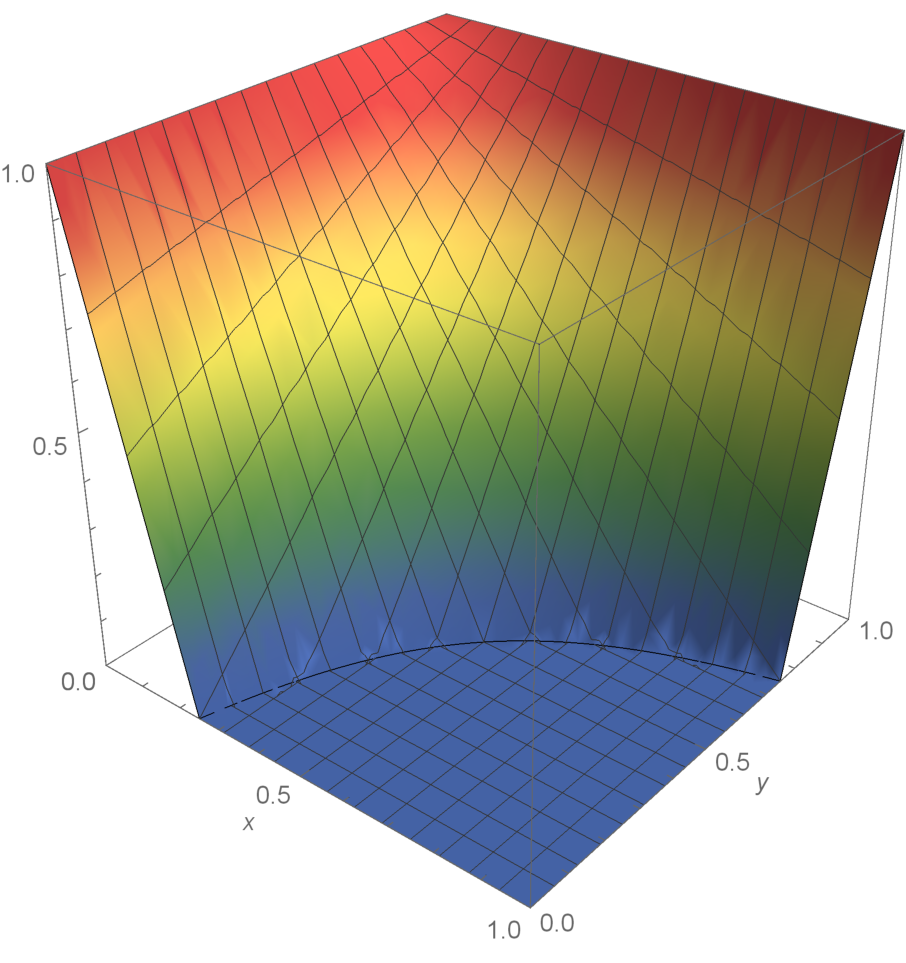
\includegraphics[width=4cm]{c1.pdf} } \quad
		\subfloat[$(I_{\bf RC}^{\frac{1}{4}})_{\varphi}$ with $\varphi(x)=x^2$]{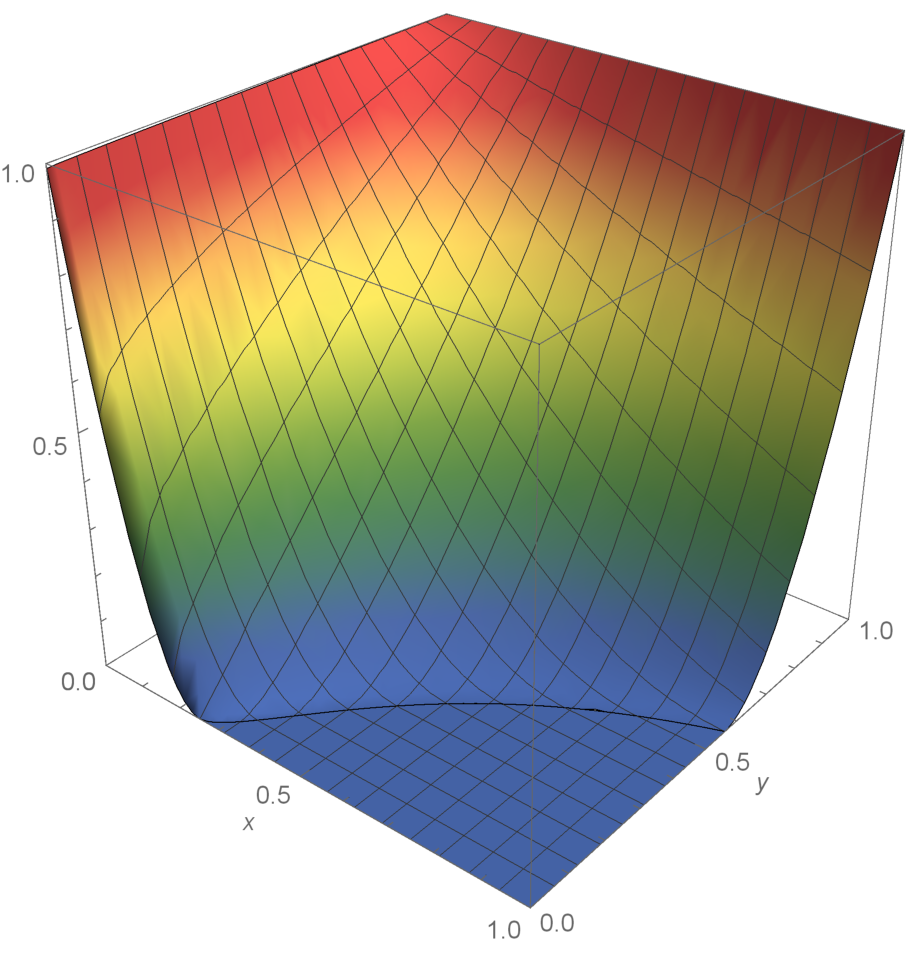
\includegraphics[width=4cm]{c2.pdf} } \quad
		\subfloat[$(I_{\bf RC}^{\frac{1}{4}})_{\varphi}$ with $\varphi(x)=\sqrt{x}$]{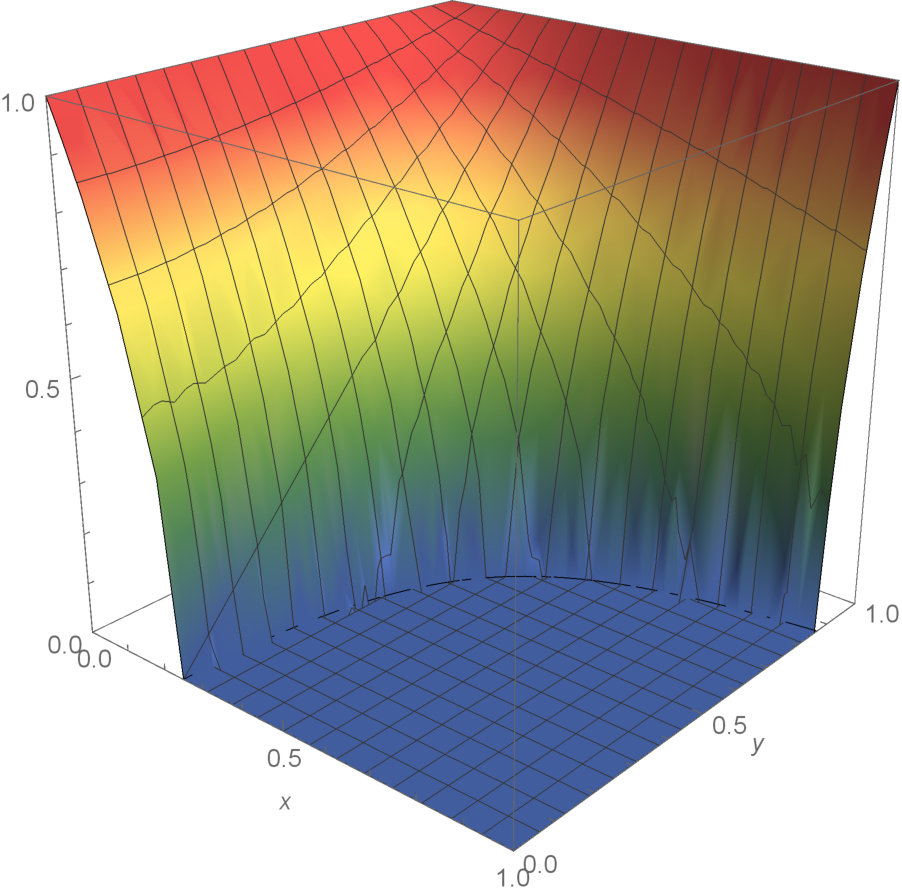
\includegraphics[width=4cm]{c3.pdf} }\\
		\caption{Plot of the fuzzy implication function $I_{\bf RC}^e$ with $e=\frac{1}{4}$ jointly with two of its $\varphi$-pseudo conjugates.}\label{(f,e)conj}
	\end{figure}
\end{example}

\section{Characterizations of generalized $(h,e)$-implications}\label{section:characterization(h,e)}

In this section we use the representation theorem of generalized $(h,e)$-implications and the characterizations of $(f,e)$ and $(g,e)$-implications presented in Section \ref{section:characterizations(f,e)&(g,e)} in order to provide an axiomatic characterization for generalized $(h,e)$-implications.

The idea of the proofs is to translate the properties that appear in the characterizations of the $(f,e)$ and $(g,e)$-implications to properties related to generalized $(h,e)$-implications by using the representation theorem of this family. We have seen that the characterization of $(f,e)$-implications is significantly different when $f(0)$ is finite or not. For this reason, we distinguish two cases also for the characterization of generalized $(h,e)$-implications.

First of all, we need to study when the generalized $(h,e)$-implications satisfy the new properties of fuzzy implication functions introduced in this work, \LIex and \LIey with respect to the product t-norm $\TP$.

\begin{proposition} Let $h$ be a generalized $h$-generator and $e \in (0,1)$. Then
	
	\begin{enumerate}[label=(\roman*)]
		\item $I^{h_g,e}$ satisfies \LIey with respect to $\TP$.
		\item It holds that $I^{h_g,e}(xy,z)=I^{h_g,e}(ex,I^{h_g,e}(y,z))$ for all $x,y \in [0,1]$ and $z \in [e,1]$.
		\item $I^{h_g,e}$ satisfies \LIex with respect to $\TP$ if and only if $h(0)=-\infty$.
	\end{enumerate}
	\label{propietats2(h,e)}
\end{proposition}
\begin{proof} Let us consider $e\in (0,1)$, $I$ a generalized $(h,e)$-implication and $h$ a generator of $I$.
	\begin{enumerate}[label=(\roman*)] 
		\item On the one hand,
		$$I(xy,z)= \left\{ \begin{array}{lcl}
			1 &   \hbox{if}  & x=0 \hbox{ or } y=0, \\
			h^{(-1)}\left( \frac{xy}{e}h(z) \right) &   \hbox{if}  & x,y>0 \hbox{ and } z \leq e, \\
			h^{-1}\left( \frac{e}{xy}h(z) \right) &   \hbox{if}  & x,y>0 \hbox{ and } z > e. \\
		\end{array}
		\right.
		$$
		Now, in order to prove the equality $I(xy,z)=I(x,I(ey,z))$ let us distinguish different cases:
		\begin{itemize}
			\item If $x=0$ we have that
			$$I(0,z)=1=I(0,I(ey,z)), \hspace{0.5cm} \text{ for all } y,z \in [0,1].$$
			\item If $y=0$ it holds that
			$$I(0,z)=1=I(x,1)=I(x,I(0,z)), \hspace{0.5cm} \text{ for all } y,z \in [0,1].$$
			\item If $x,y>0$ and $z \leq e$ then
			$$I(x,I(ey,z))=I(x,h^{(-1)}(yh(z))).$$
			We have that $yh(z) \geq h(z) > h(0)$ and consequently $h^{(-1)}(yh(z))=h^{-1}(yh(z))$. Moreover, since $h$ is strictly increasing, $h^{-1}$ is increasing in $(h(0),0]$ and 
			$$h(z) \leq h(e)=0 \Rightarrow yh(z) \leq 0 \Rightarrow h^{-1}(yh(z)) \leq h^{-1}(0)=e.$$
			Thus,
			\begin{eqnarray*}
			I(x,I(ey,z)) &=& I(x,h^{-1}(yh(z))) = h^{(-1)} \left( \frac{x}{e}(h \circ h^{-1})(yh(z))\right) \\
			&=& h^{(-1)} \left( \frac{xy}{e}h(z)\right) = I(xy,z).
			\end{eqnarray*}
			\item If $x,y>0$ and $z>e$ then
			$$I(x,I(ey,z))=I\left(x,h^{-1}\left(\frac{h(z)}{y}\right)\right).$$
			Again, by the strictly increasing nature of $h$, $h^{-1}$ is strictly increasing in $(0,+\infty)$ and then
			$$ \frac{1}{y} \geq 1 \Rightarrow \frac{h(z)}{y} \geq h(z) > h(e)=0 \Rightarrow h^{-1} \left( \frac{h(z)}{y}\right) > h^{-1}(0)=e.$$
			Hence,
			\begin{eqnarray*}
			I(x,I(ey,z))&=&I\left(x,h^{-1}\left(\frac{h(z)}{y}\right)\right) = h^{-1}\left(\frac{e}{x}(h \circ h^{-1})\left(\frac{h(z)}{y}\right)\right)\\
			&=&I\left(\frac{e}{xy}h(z)\right)=I(xy,z).
			\end{eqnarray*}
		\end{itemize}
		\item We have to prove that $I(xy,z)=I(ex,I(y,z))$ for all $x,y\in [0,1]$ and $z\geq e$.
		\begin{itemize}
			\item If $x=0$ we have that
			$$I(0,z)=1=I(0,I(y,z)), \hspace{0.5cm} \text{ for all } y,z \in [0,1].$$
			\item If $y=0$ it holds that
			$$I(0,z)=1=I(ex,1)=I(ex,I(0,z)), \hspace{0.5cm} \text{ for all } y,z \in [0,1].$$
			\item If $x,y>0$ and $z=e$ then since $h(e)=0$ we have that
			$$I(ex,I(y,e))=I\left(ex,h^{(-1)}\left(\frac{y}{e}h(e)\right)\right) = I(ex,e)=h^{(-1)}(xh(e))=e.$$
			On the other hand, $I(xy,e)=h^{(-1)}\left(\frac{xy}{e}h(e)\right)=e$.
			\item If $x,y>0$ and $z>e$ then
			$$I(ex,I(y,z)) = I\left(ex, h^{-1} \left(\frac{e}{y}h(z)\right)\right).$$
			Now, since $h$ is strictly increasing, $h^{-1}$ is strictly increasing in $(0,+\infty)$ and we get that
			$$\frac{e}{y} \geq e \Rightarrow \frac{e}{y}h(z) \geq eh(z) > eh(e) =0 \Rightarrow h^{-1}\left(\frac{e}{y}h(z)\right) > h^{-1}(0)=e,$$
			and then
			\begin{eqnarray*}
			I(ex,I(y,z)) &=& I\left(ex, h^{-1} \left(\frac{e}{y}h(z)\right)\right) = I\left(\frac{1}{x}(h \circ h^{-1})\left(\frac{e}{y}h(z)\right)\right) \\
			&=& I\left(\frac{e}{xy}h(z)\right)=I(xy,z).
			\end{eqnarray*}
		\end{itemize}
		\item First, let $h$ be a generalized $h$-generator with $h(0) > -\infty$. Let us consider $x \in (0,1)$, $y \in (0,1]$ and $z \in [0,e)$ such that $yh(z) < eh(0)$, then
		$$I(ex,I(y,z))=I\left(ex,h^{(-1)}\left(\frac{y}{e}h(z)\right)\right) = I(ex,0)=h^{(-1)}(xh(0))=h^{-1}(xh(0)).$$
		On the other hand, we can find an $x\in(0,1)$ small enough such that $xyh(z)>eh(0)$ and we get that
		$$I(xy,z)=h^{(-1)}\left(\frac{xy}{e}h(z)\right)=h^{-1}\left(\frac{xy}{e}h(z)\right).$$
		But since $h^{-1}$ is strictly increasing in $[h(0),0)$ we have that
		$$\frac{yh(z)}{e} < h(0) \Rightarrow \frac{xyh(z)}{e} <xh(0) \Rightarrow h^{-1}\left(\frac{xyh(z)}{e}\right) < h^{-1}(xh(0)).$$
		Thus, $I$ does not satisfy \LIex with respect to $\TP$. On the other hand, consider $h$ a generalized $h$-generator with $h(0)=-\infty$, then $h^{(-1)}=h^{-1}$. Considering Point (ii), we only need to prove that $I$ satisfies $I(xy,z)=I(ex,I(y,z))$ for all $x,y\in[0,1]$ and $z \in [0,e)$. First
		$$I(ex,I(y,z))= I\left(ex,h^{-1}\left(\frac{y}{e}h(z)\right)\right).$$
		Now, since $\frac{y}{e}h(z) \leq 0$, we have that $h^{-1}\left(\frac{y}{e}h(z)\right) \leq h^{-1}(0)=e$ due to the increasingness of $h^{-1}$. Thus,
		\begin{eqnarray*}
		I(ex,I(y,z)) &=& I\left(ex,h^{-1}\left(\frac{y}{e}h(z)\right)\right) = h^{-1}\left(x (h \circ h^{-1})\left(\frac{y}{e}h(z)\right)\right)\\
		&=&h^{-1}\left(\frac{xy}{e}h(z)\right)=I(xy,z).
		\end{eqnarray*}
	\end{enumerate}
\end{proof}

At this point and using the previous results, we can obtain the characterization of generalized $(h,e)$-implications in both cases.

First of all, we will consider the case of a generalized $(h,e)$-implication with $h(0) > - \infty$. 

\begin{theorem}\label{charach(h,e)fin} Let $I:[0,1]^2 \to [0,1]$ be a binary function and $ e \in (0,1)$. Then the following statements are equivalent:
	
	\begin{enumerate}[label=(\roman*)]
		\item $I$ is a generalized $(h,e)$-implication with respect to $e$ with $h(0)> - \infty$.
		\item $I$ satisfies the following properties:
		
		\begin{enumerate}[label=\arabic*.]
			\item $I$ is continuous on the points $(x,y)$ with $x> 0$ and $y\geq e$ and $(0,y)$ with $y>e$.
			\item $I(x,y)=1 \Leftrightarrow x=0 \text{ or } y=1$.
			\item For all $k \in (0,1]$, $I(k,y)$ is strictly increasing for all $y \in[0,1]$ with $I(k,e)=e$.
			\item $N_I$ is a fuzzy negation such that $N_I(e)=0$, continuous on $(0,e]$, strictly decreasing in $(0,e)$ and $\displaystyle \lim_{x \to 0^+}N_I(x)=e$.
			\item $I$ satisfies \LIey with respect to $\TP$.
			\item $I$ satisfies $I(xy,z)=I(ex,I(y,z))$ for all $x,y \in [0,1]$ and $z\geq e$.
		\end{enumerate}
	\end{enumerate}
	Moreover, in this case the generalized $h$-generator is given by
	$$h(x)=\left\{ \begin{array}{lcl}
		-e &   \hbox{if}  & x=0, \\[0.7em]
		-N_I^{-1}(x) &  \hbox{if} & 0<x \leq e, \\[0.7em]
		\displaystyle \frac{h_x^{-1}(k)}{e^2}&  \hbox{if}  & e<x<k, \\[0.7em]
		\displaystyle \frac{1}{h_k^{-1}(x)}  &  \hbox{if}  & k \leq x \leq 1,
	\end{array}
	\right.
	$$
	for some $k \in (e,1)$ where $h_k(x)=I(x,k)$ and $h_{\bullet}^{-1}(k):(e,k)\to [0,e]$ is the function that assigns $h_y^{-1}(k)$ to some $ y \in (e,k)$.
\end{theorem}
\begin{proof}
	{\bf (ii)$\Rightarrow$(i)} Let us define the following functions $I_1,I_2:[0,1]^2 \to [0,1]$ given by
	$$I_1(x,y)=\left\{ \begin{array}{ccl}
		1 &   \hbox{if}  & x=0, \\
		\displaystyle \frac{I(x,ey)}{e} &  \hbox{if} & x>0, \\
	\end{array}
	\right.
	\hspace{0.5cm}
	I_2(x,y)=\left\{ \begin{array}{ccl}
		1 &   \hbox{if}  & x=0, \\
		\displaystyle \frac{I(x,e+(1-e)y)-e}{1-e} &  \hbox{if} & x>0. \\
	\end{array}
	\right.
	$$
	First, let us check that $I_1$ is an $(f,e)$-implication with $f(0)< +\infty$:
	\begin{itemize}
		\item $I_1$ is a well-defined function. Indeed, $\frac{I(x,ey)}{e} \geq 0$ and $\frac{I(x,ey)}{e}\leq 1$ since $I(x,ey) \leq e$ by Property (ii)-3.
		\item $N_{I_1}$ is given by
		$$N_{I_1}(x)=\left\{ \begin{array}{ccl}
			1 &   \hbox{if}  & x=0, \\
			\frac{N_I(x)}{e} &  \hbox{if} & x>0, \\
		\end{array}
		\right.
		$$
		and it is a fuzzy negation since $N_{I_1}(0)=1$ by construction, $N_{I_1}(1)=\frac{N_I(1)}{e}=0$ by Property (ii)-4 and it is decreasing due to the decreasingness of $N_I$ guaranteed also by Property (ii)-4.
		\item $N_{I_1}$ is continuous for all $x>0$ by Property (ii)-4 and at $x=0$ because $N_{I_1}(0)=1$ and 
		$$\lim_{x \to 0^+}N_{I_1}(x)=\lim_{x \to 0^+}\frac{N_I(x)}{e}=\frac{e}{e}=1,$$
		by Property (ii)-4.
		\item  $N_{I_1}$ is strictly decreasing in $(0,e)$ since $N_I$ is strictly decreasing in $(0,e)$ also by Property (ii)-4. 
		\item $N_{I_1}(e)=\frac{N_I(e)}{e}=\frac{0}{e}=0$ by Property (ii)-4.
		\item Let us prove that $I_1$ satisfies \LIey with respect to $\TP$. Let us first consider $x,y,z\in [0,1]$ with $x,y>0$. Since $I$ satisfies \LIey with respect to $\TP$ we have that
		\begin{eqnarray*}
		I_1(xy,z) &=& \frac{I(xy,ez)}{e} = \frac{I(x,I(ey,ez))}{e} = \frac{I\left(x, \frac{eI(ey,ez)}{e}\right)}{e}\\
		&=&\frac{I(x,eI_1(ey,z))}{e} =I_1(x,I_1(ey,z)).
		\end{eqnarray*}
		Finally, note that if $x=0$, $I_1(xy,z)=I_1(0,z)=1=I_1(0,I_1(ey,z))=I_1(x,I_1(ey,z))$, and if $y=0$, $I_1(xy,z)=I_1(0,z)=1=I_1(x,1)=I_1(x,I_1(0,z))=I_1(x,I_1(ey,z))$. Notice that in this last equality we have used that $I_1(x,1)=\frac{I(x,e)}{e}=\frac{e}{e}=1$ by Property (ii)-3.
	\end{itemize}
	Thus, we have proved by Theorem \ref{caractf0fin} that $I_1$ is an $(f,e)$-implication with $f(0) < +\infty$. In this case, moreover, we have that the $f$-generator is given by
	$$f(x)=N_{I_1}^{(-1)}(x)= \left\{ \begin{array}{ccl}
		N_{I_1}^{-1}(x) &   \hbox{if}  & x>0, \\
		e &  \hbox{if} & x=0,
	\end{array}
	\right. =
	\left\{ \begin{array}{ccl}
		N_{I}^{-1}(ex) &   \hbox{if}  & x>0, \\
		e &  \hbox{if} & x=0.
	\end{array}
	\right.
	$$
	Let us check now that $I_2$ is a $(g,e)$-implication with $g(1)=+\infty$.
	\begin{itemize}
		\item $I_2$ is a well-defined function since by Property (ii)-3, $I(x,e+(1-e)y)\geq e$.
		\item Let us prove that $I_2$ is continuous except at $(0,0)$. Since $I(x,e+(1-e)y)$ is continuous for all $x>0$ by Property (ii)-1, $I_2$ is continuous for all $x>0$. Moreover $I_2$ is also continuous on $(0,y)$ with $y>0$ since in this case, $I_2(0,y)=1$ and $\displaystyle \lim_{x \to 0^+}I_2(x,y)=\frac{1-e}{1-e}=1$ due to the continuity of $I$ at points $(0,y)$ with $y>e$. On the other hand, $I_2$ is not continuous on $(0,0)$ because $I_2(0,0)=1$ but $\displaystyle \lim_{x \to 0^+} I_2(x,0)=\lim_{x \to 0^+}\frac{I(x,e)-e}{1-e}=0$ by Property (ii)-3.
		\item Let us prove that $I_2(x,y)=1 \Leftrightarrow x=0 \hbox{ or } y=1$. First, if $x=0$, $I_2(0,y)=1$ by construction. Now, if $x>0$, we have that
		$$I_2(x,y)=1 \Leftrightarrow I(x,e+y(1-e))-e=1-e \Leftrightarrow I(x,e+y(1-e))=1.$$
		By Property (ii)-2, this happens if and only if $x=0$ or $e+y(1-e)=1 \Leftrightarrow y=1$.
		\item $I_2$ satisfies \LIex with respect to \TP. Indeed, by using Property (ii)-6, for $x,y,z \in [0,1]$ with $x,y>0$ we have that
		\begin{eqnarray*}
			I_2(xy,z) &=&  \frac{I(xy,e+(1-e)z)-e}{1-e} =  \frac{I(ex,I(y,e+(1-e)z))-e}{1-e} \\
			&=& \frac{I(ex,e+(1-e)I_2(y,z))-e}{1-e} = I_2(ex,I_2(y,z)).
		\end{eqnarray*}
		Note again that if $x=0$, $I_2(0,I_2(y,z))=1=I_2(0,z)$ and if $y=0$, $I_2(ex,I_2(0,z))=I_2(ex,1)=1=I_2(0,z)$. Then $I_2$ satisfies \LIex with \TP.
		\item Finally, let us prove that $I_2$ satisfies \LIey with respect to $\TP$. By Property (ii)-5, for $x,y,z \in [0,1]$ with $x,y>0$ we have that
		\begin{eqnarray*}
			I_2(xy,z)&=& \frac{I(xy,e+(1-e)z)-e}{1-e} =\frac{I(x,I(ey,e+(1-e)z))-e}{1-e} \\
			&=&\frac{I(x,e+(1-e)I_2(ey,z))-e}{1-e} = I_2(x,I_2(ey,z)).
		\end{eqnarray*}
		If $x=0$, $I_2(0,I_2(ey,z))=1=I_2(0,z)$ and if $y=0$, $I_2(x,I_2(0,z))=I_2(x,1)=1=I_2(0,z)$. Then $I_2$ satisfies \LIey with \TP.
	\end{itemize}
	Thus, we have proved by Theorem \ref{caractg1fin} that $I_2$ is a $(g,e)$-implication with $g(1)=+ \infty$. In this case, moreover, we have that the $g$-generator is given by
	$$g(x)=\left\{ \begin{array}{ccl}
		\displaystyle \frac{1}{\hat{h}_k^{-1}(x)} &   \hbox{if}  & k \leq x \leq 1, \\[1em]
		\displaystyle\frac{\hat{h}_x^{-1}(k)}{e^2} &  \hbox{if} & 0<x<k, \\[1em]
		0 &  \hbox{if} & x=0, 
	\end{array}
	\right.
	$$
	where $k\in(0,1)$, $\hat{h}_k(x)=I_2(x,k)=\frac{I(x,e+(1-e)k)-e}{1-e}$ and $\hat{h}_{\bullet}^{-1}(k):(0,k)\to [0,e]$ is the function that assigns $\hat{h}_y^{-1}(k)$ to some $ y \in (0,k)$. Let us rewrite $g$ in terms of $I$:
	\begin{itemize}
		\item  Consider $ k \leq x \leq 1$, then we have that
		\begin{eqnarray*}
			\hat{h}_k^{-1}(x)=x' &\Leftrightarrow & I_2(x',k)=x \Leftrightarrow \frac{I(x',e+(1-e)k)-e}{1-e}=x \\
			&\Leftrightarrow& I(x',e+(1-e)k)=e+(1-e)x  \\
			&\Leftrightarrow&  h^{-1}_{e+(1-e)k}(e+(1-e)x)=x'.
		\end{eqnarray*}
		where $h_k(x)=I(x,k)$.
		\item Let us assume $0<x<k$, we get that $\hat{h}_x^{-1}(k)=h_{e+(1-e)x}(e+(1-e)k)$ analogously.
	\end{itemize}
	Thus,
	$$g(x)=\left\{ \begin{array}{ccl}
		\displaystyle \frac{1}{h_{e+(1-e)k}^{-1}(e+(1-e)x)} &   \hbox{if}  & k \leq x \leq 1, \\[1em]
		\displaystyle \frac{h_{e+(1-e)x}^{-1}(e+(1-e)k)}{e^2} &  \hbox{if} & 0<x<k, \\[1em]
		0 &  \hbox{if} & x=0, 
	\end{array}
	\right.
	$$
	for some $k \in (0,1)$ where $h_k(x)=I(x,k)$.\\
	
	Taking into account these two fuzzy implication functions, it can be easily verified that $I$ can be written as
	$$I(x,y)= \left\{ \begin{array}{lcl}
		1 &   \hbox{if}  & x=0, \\
		eI_1(x,\frac{y}{e}) &  \hbox{if} & x>0 \hbox{ and } y \leq e, \\
		e+(1-e)I_2\left(x,\frac{y-e}{1-e}\right) &  \hbox{if} & x>0 \hbox{ and } y>e. \\
	\end{array}
	\right.
	$$
	Hence by Theorem \ref{ThmRep(h,e)} we know that $I$ is a generalized $(h,e)$-implication with respect to e with $h(0)> - \infty$. Moreover, the generalized $h$-generator is given by
	$$h(x)=\left\{ \begin{array}{ccl}
		-e &   \hbox{if}  & x=0, \\[1em]
		-N_{I}^{-1}(x) &   \hbox{if}  & 0<x \leq e, \\[1em]
		\displaystyle \frac{h_x^{-1}(e+(1-e)k)}{e^2} &   \hbox{if}  & e<x<e+(1-e)k, \\[1em]
		\displaystyle \frac{1}{h_{e+(1-e)k}^{-1}(x)} &   \hbox{if}  & e+(1-e)k\leq x\leq 1, \\
	\end{array}
	\right.
	$$
	for some $k\in (0,1)$. Equivalently, for some $k\in (e,1)$, $h$ is given by
	$$h(x)=\left\{ \begin{array}{ccl}
		-e &   \hbox{if}  & x=0, \\[1em]
		-N_{I}^{-1}(x) &   \hbox{if}  & 0<x \leq e, \\[1em]
		\displaystyle \frac{h_x^{-1}(k)}{e^2} &   \hbox{if}  & e<x<k, \\[1em]
		\displaystyle \frac{1}{h_{k}^{-1}(x)} &   \hbox{if}  & k\leq x\leq 1. \\[1em]
	\end{array}
	\right.
	$$
	
	{\bf (i)$ \Rightarrow$(ii)} Let us consider $I$ a generalized $(h,e)$-implication with respect to $e$ with $h(0)>-\infty$. We know that $I$ satisfies the Properties (ii)-1 to (ii)-6 by Theorem \ref{th:AddProp(h,e)} and Proposition \ref{propietats2(h,e)}.
\end{proof}

On the other hand, we have a similar characterization theorem for $(h,e)$-implications with $h(0)=-\infty$ considering the characterization of $(f,e)$-implications with $f(0)=+\infty$.\\

\begin{theorem}\label{th:(h,e)h(0)-inf} Let $I:[0,1]^2 \to [0,1]$ be a binary function and $e \in (0,1)$. Then the following statements are equivalent:	\begin{enumerate}[label=(\roman*)]
		\item $I$ is a generalized $(h,e)$-implication with respect to $e$ with $h(0)= - \infty$.
		\item $I$ satisfies the following properties:
		\begin{enumerate}[label = \arabic*.]
			\item $I$ is continuous except at the points $(0,y)$ with $y\leq e$.
			\item $I(x,y)=1 \Leftrightarrow x=0 \text{ or } y=1$.
			\item For all $k \in (0,1]$, $I(k,x)$ is strictly increasing with $I(k,e)=e$.
			\item $\displaystyle \lim_{x \to 0^+} I(x,y)=e$ for all $0<y \leq e$.
			\item $I$ satisfies \LIey and \LIex with respect to $\TP$ for all $x,y,z \in [0,1]$.
		\end{enumerate}
	\end{enumerate}
		Moreover, in this case the $h$ generalized $h$-generator is given by
		$$h(x)=\left\{ \begin{array}{ccl}
			- \infty &  \hbox{if} & x=0, \\[1em]             
			\displaystyle -\frac{e}{h_{x}^{-1}(k_1)} &  \hbox{if} & 0<x<k_1, \\[1em]
			\displaystyle -\frac{h_{k_1}^{-1}(x)}{e} &   \hbox{if}  & k_1 \leq x \leq e, \\[1em]
			\displaystyle \frac{h_x^{-1}(k_2)}{e^2} &   \hbox{if}  & e<x<k_2, \\[1em]
			\displaystyle \frac{1}{h_{k_2}^{-1}(x)} &   \hbox{if}  & k_2\leq x\leq 1, \\[1em]
		\end{array}
		\right.
		$$
		for some $k_1 \in (0,e)$ and $k_2 \in (e,1)$ where $h_{k_i}(x)=I(x,k_i)$ for $i \in \{1,2\}$, $h_{\bullet}^{-1}(k_1):(0,k_1)\to [0,e]$ is the function that assigns $h_y^{-1}(k_1)$ to some $ y \in (0,k_1)$, and $h_{\bullet}^{-1}(k_2):(e,k_2)\to [0,e]$ is the function that assigns $h_y^{-1}(k_2)$ to some $ y \in (e,k_2)$.
\end{theorem}
\begin{proof}
	\begin{description}
	\item[(ii) $\Rightarrow$ (i)] Let us define the functions $I_1,I_2:[0,1] \to [0,1]$ given by
	$$I_1(x,y)=\left\{ \begin{array}{ccl}
		1 &   \hbox{if}  & x=0, \\
		\displaystyle \frac{I(x,ey)}{e} &  \hbox{if} & x>0, \\
	\end{array}
	\right.
	\hspace{0.5cm}
	I_2(x,y)=\left\{ \begin{array}{ccl}
		1 &   \hbox{if}  & x=0, \\
		\displaystyle \frac{I(x,e+(1-e)y)-e}{1-e} &  \hbox{if} & x>0. \\
	\end{array}
	\right.
	$$
	Now, let us prove that $I_1$ is an $(f,e)$-implication with $f(0) = +\infty$:
	\begin{itemize}
		\item $I_1$ is a well-defined function since we have that $\frac{I(x,ey)}{e}\geq 0$ and by Property (ii)-3, $\frac{I(x,ey)}{e} \leq 1$.
		\item $I_1$ is continuous except at $(0,0)$. Since $I(x,ey)$ is continuous for all $x>0$ by Property (ii)-1, $I_1$ is continuous for all $x>0$. Furthermore, $I_1$ is also continuous on $(0,y)$ with $y>0$ since $I(0,y)=1$ and by Property (ii)-4 we have that 
		$$\lim_{x \to 0^+} I_1(x,y)= \lim_{x \to 0^+} \frac{I(x,ey)}{e} = \frac{e}{e}=1.$$
		On the other hand $I_1$ is not continuous on $(0,0)$ since $I$ is not continuous on $(0,0)$ and
		$$ \lim_{(x,y) \to (0,0)} I_1(x,y) = \lim_{(x,y) \to (0,0)} \frac{I(x,ey)}{e}.$$
		\item  $I_1(x,y)=1 \Leftrightarrow x=0 \hbox{ or } y=1$. First, if $x=0$, $I_1(0,y)=1$ by construction. Now, if $x>0$, we have that
		$$I_1(x,y)=1 \Leftrightarrow I(x,ey)=e.$$
		By Property (ii)-3, this holds if, and only if, $y=1$.
		\item  Let us prove that $I_1$ satisfies \LIex with respect to $\TP$.  For $x,y,z \in[0,1]$ with $x,y>0$, by Property (ii)-5, we have that
		\begin{eqnarray*}
		I_1(xy,z) &=& \frac{I(xy,ez)}{e} = \frac{I\left(ex,I(y,ez)\right)}{e} = \frac{I\left(ex,e\frac{I(y,ez)}{e}\right)}{e}\\
		&=&\frac{I(ex,eI_1(y,z))}{e} = I_1(ex,I_1(y,z)).
		\end{eqnarray*}
		Note that if $x=0$, $I_1(0,I_1(y,z))=1=I_1(0,z)$ and if $y=0$, $I_1(ex,I_1(0,z))=I_1(ex,1)=1=I_1(0,z)$. Then $I_1$ satisfies  \LIex with respect to $\TP$.
		\item  Finally, let us prove that $I_1$ satisfies \LIey with respect to $\TP$. If we consider $x,y,z \in [0,1]$ such that $x,y>0$, again considering Property (ii)-5 we have that
		\begin{eqnarray*}
		I_1(xy,z) &=& \frac{I(xy,ez)}{e} = \frac{I\left(x,I(ey,ez)\right)}{e} = \frac{I\left(x,e\frac{I(ey,ez)}{e}\right)}{e} \\
		&=& \frac{I(x,eI_1(ey,z))}{e} = I_1(x,I_1(ey,z)).
		\end{eqnarray*}
		Again we have that if $x=0$, $I_1(0,I_1(ey,z))=1=I_1(0,z)$ and if $y=0$, $I_1(x,I_1(0,z))=I_1(x,1)=1=I_1(0,z)$. Thus, $I_1$ satisfies \LIey with respect to $\TP$.
	\end{itemize}
	Then, we have proved by Theorem \ref{caractf0inf} that $I_1$ is an $(f,e)$-implication with $f(0)= +\infty$. In this case, moreover, we have that the $f$-generator is given by
	$$f(x)=\left\{ \begin{array}{ccl}
		\displaystyle \frac{\Hat{h}_k^{-1}(x)}{e} &   \hbox{if}  & k \leq x \leq 1, \\[1em]
		\displaystyle \frac{e}{\Hat{h}_x^{-1}(k)} &  \hbox{if} & 0<x<k, \\[1em]
		+ \infty &  \hbox{if} & x=0, \\
	\end{array}
	\right.
	$$
	for some $k\in(0,1)$ where $\Hat{h}_k(x)=I_1(x,k)=\frac{I(x,ek)}{e}$. Now, let us rewrite $f$ in terms of $I$.
	\begin{itemize}
		\item  If $ k \leq x \leq 1$ then
		$$ \Hat{h}_k^{-1}(x)=x' \Leftrightarrow I_1(x',k)=x \Leftrightarrow I(x',ek)=ex \Leftrightarrow h_{ek}^{-1}(ex)=x',$$
		with $h_k(x)=I(x,k).$
		\item  If $ 0 \leq x \leq k$ then analogously we obtain that $\Hat{h}_x^{-1}(k)=h^{-1}_{ex}(ek)$.
	\end{itemize}
	Then,
	$$f(x)=\left\{ \begin{array}{ccl}
		\displaystyle\frac{h_{ek}^{-1}(ex)}{e} &   \hbox{if}  & k \leq x \leq 1, \\[1em]
		\displaystyle \frac{e}{h_{ex}^{-1}(ek)} &  \hbox{if} & 0<x<k, \\[1em]
		+ \infty &  \hbox{if} & x=0, \\
	\end{array}
	\right.
	$$
	for some $k \in (0,1)$ and $h_k(x)=I(x,k)$.
	
	On the other hand, in order to check that $I_2$ is a $(g,e)$-implication with $g(1)=+\infty$  we can consider the same corresponding argument as in the proof of Theorem \ref{charach(h,e)fin}.
	
	Now, considering the fuzzy implication functions $I_1$ and $I_2$, we have that $I$ can be written as follows
	$$I(x,y)= \left\{ \begin{array}{lcl}
		1 &   \hbox{if}  & x=0, \\
		eI_1(x,\frac{y}{e}) &  \hbox{if} & x>0 \hbox{ and } y \leq e, \\
		e+(1-e)I_2\left(x,\frac{y-e}{1-e}\right) &  \hbox{if} & x>0 \hbox{ and } y>e. \\
	\end{array}
	\right.
	$$
	Thus, by Theorem \ref{ThmRep(h,e)} we obtain that $I$ is a generalized $(h,e)$-implication with respect to $e$ with $h(0)=-\infty$. Moreover, the generalized $h$-generator is given by
	$$h(x)=\left\{ \begin{array}{ccl}
		- \infty &  \hbox{if} & x=0, \\[1em]
		\displaystyle -\frac{e}{h_{x}^{-1}(ek_1)} &  \hbox{if} & 0<x<ek_1, \\[1em]
		\displaystyle -\frac{h_{ek_1}^{-1}(x)}{e} &   \hbox{if}  & ek_1 \leq x \leq e, \\[1em]        
		\displaystyle \frac{h_x^{-1}(e+(1-e)k_2)}{e^2} &   \hbox{if}  & e<x<e+(1-e)k_2, \\[1em]
		\displaystyle \frac{1}{h_{e+(1-e)k_2}^{-1}(x)} &   \hbox{if}  & e+(1-e)k_2\leq x\leq 1, \\
	\end{array}
	\right.
	$$
	where $k_1,k_2 \in (0,1)$ and $h_k(x)=I(x,k)$. Equivalently, for some $k_1 \in (0,e)$ and $k_2 \in (e,1)$, $h$ is given by
	$$h(x)=\left\{ \begin{array}{ccl}
		- \infty &  \hbox{if} & x=0, \\  [1em]           
		\displaystyle -\frac{e}{h_{x}^{-1}(k_1)} &  \hbox{if} & 0<x<k_1, \\[1em]
		\displaystyle -\frac{h_{k_1}^{-1}(x)}{e} &   \hbox{if}  & k_1 \leq x \leq e, \\[1em]
		\displaystyle \frac{h_x^{-1}(k_2)}{e^2} &   \hbox{if}  & e<x<k_2, \\[1em]
		\displaystyle \frac{1}{h_{k_2}^{-1}(x)} &   \hbox{if}  & k_2\leq x\leq 1. \\[1em]
	\end{array}
	\right.
	$$
	\item[(i)$\Rightarrow$(ii)] Let us consider $I$ a generalized $(h,e)$-implication with respect to $e$ with $h(0)= -\infty$. Then, $I$ satisfies Properties 1 to 5 by Theorem \ref{th:AddProp(h,e)} and Proposition \ref{propietats2(h,e)}.
	\end{description}
\end{proof}

To conclude this section we provide an example that shows how Theorems \ref{caractg1fin} and \ref{th:(h,e)h(0)-inf} can be used to prove that a function $I: [0,1]^2 \to [0,1]$ is a generalized $(h,e)$-implication and to obtain the corresponding generator.

\begin{example}\label{example:characterization(h,e)-implications}
	Let us consider the function $I: [0,1]^2 \to [0,1]$ given by
	$$
	I(x,y)=\left\{ \begin{array}{cl}
		1 &   \hbox{if }   x=0, \\
		\frac{y^{2x}}{(1-y)^{2x}+y^{2x}} &   \hbox{if }   x>0 \text{ and } y \leq \frac{1}{2}, \\
		\frac{y^{\frac{1}{2x}}}{(1-y)^{\frac{1}{2x}} + y^{\frac{1}{2x}}} &   \hbox{if }    x>0 \text{ and } y > \frac{1}{2}. 
	\end{array}
	\right.
	$$
	It is easy to check that this function fulfills all the properties in (ii)-Theorem \ref{th:(h,e)h(0)-inf} with $e=\frac{1}{2}$ so it is a generalized $(h,e)$-implication with respect to $\frac{1}{2}$. On the other hand, if we consider $k_1 \in \left(0,\frac{1}{2}\right)$ and $k_2 \in \left(\frac{1}{2},1\right)$ we have
	$$
	h_{k_1}(x)=I(x,k_1) =\left\{ \begin{array}{cl}
		1 &   \hbox{if }   x=0, \\
		\frac{k_1^{2x}}{(1-k_1)^{2x}+k_1^{2x}} &   \hbox{if }   x>0, \\
	\end{array}
	\right.
	\quad
	h_{k_1}^{-1}(x)= \left\{ \begin{array}{cl}
		0 &   \hbox{if }   x=1, \\
		\frac{1}{2 \cdot \ln \left(\frac{k_1}{1-k_1}\right)} \ln \left(\frac{x}{1-x}\right)&   \hbox{if }   x<1, \\
	\end{array}
	\right.
	$$
	$$
	h_{k_2}(x)=I(x,k_2) =\left\{ \begin{array}{cl}
		1 &   \hbox{if }   x=0, \\
		\frac{k_2^{\frac{1}{2x}}}{(1-k_2)^{\frac{1}{2x}} + k_2^{\frac{1}{2x}}} &   \hbox{if }   x>0, \\
	\end{array}
	\right.
	\quad
	h_{k_2}^{-1}(x)= \left\{ \begin{array}{cl}
		0 &   \hbox{if }   x=1, \\
		\frac{1}{2 \cdot \ln \left(\frac{x}{1-x}\right)} \ln \left(\frac{k_2}{1-k_2}\right) &   \hbox{if }   x<1, \\
	\end{array}
	\right.
	$$
	$$
	h_{x}^{-1}(k_1)= 	\frac{1}{2 \cdot \ln \left(\frac{x}{1-x}\right)} \ln \left(\frac{k_1}{1-k_1}\right),
	\quad
	h_{x}^{-1}(k_2)= \frac{1}{2 \cdot \ln \left(\frac{k_2}{1-k_2}\right)} \ln \left(\frac{x}{1-x}\right).
	$$
	Therefore, according to Theorem \ref{th:(h,e)h(0)-inf} an $h$-generator of $I$ is given by
	$$
	h(x)=\left\{ \begin{array}{cl}
		-\infty & \hbox{if } x=0, \\
		- \frac{1}{\ln \left( \frac{k_1}{1-k_1}\right)} \ln \left(\frac{x}{1-x}\right) &   \hbox{if }   0 < x \leq \frac{1}{2}, \\
		\frac{2}{\ln \left( \frac{k_2}{1-k_2}\right)} \ln \left(\frac{x}{1-x}\right) &   \hbox{if }   \frac{1}{2} < x \leq 1. \\
	\end{array}
	\right.
	$$
	Now, by the unicity of $h$-generators except by two multiplicative constants, if we select $c_1 = - \ln \left( \frac{k_1}{1-k_1}\right)$ and $c_2 = \frac{\ln \left( \frac{k_2}{1-k_2}\right)}{2}$ we have that an $h$-generator of $I$ is 
	$$
	\tilde{h}(x)
	=
	\left\{ \begin{array}{cl}
		c_1h(x) & \hbox{if } 0 \leq x < \frac{1}{2} \\
		c_2h(x) & \hbox{if } \frac{1}{2} \leq x \leq 1 \\	
	\end{array}
	\right.
	= \ln \left(\frac{x}{1-x}\right),
	$$
	which was the generator considered in \cite{Hlinena2013} to construct this generalized $(h,e)$-implication.
\end{example}

\section{Conclusions and future work}\label{section:conclusionshe}

In this chapter, we have provided the axiomatic characterization of the family of generalized $(h,e)$-implications. Although these fuzzy implication functions were first defined in \cite{Massanet2011A}, we have considered the more general definition given in \cite{Hlinena2013} and hence, all the results provided in \cite{Massanet2011A} have been adapted to this definition. Then, we have proved the representation theorem for $(h,e)$-implications presented in \cite{Massanet2013B}. This theorem fully determines the structure of a generalized $(h,e)$-implication given an $f$ and $g$-generator with $g(1)=+\infty$. However, in order to properly study this structure, the necessity of defining two novel families of fuzzy implication functions which are generalizations of Yager's implications has been exposed. In this sense, some additional properties of these two families of fuzzy implication functions, namely $(f,g)$ and $(g,f)$-implications, have been fully investigated. Although these properties were already presented in \cite{Massanet2013B} without proof, in this chapter we have proved all the results. Moreover, some of the results in  \cite{Massanet2013B} were not fully correct and therefore, these results have been fixed.

Further, two subfamilies of $(f,g)$ and $(g,f)$-implications, called $(f,e)$ and $(g,e)$-implications, have been deeply studied and their respective axiomatic characterization has been presented. These two families are of particular interest since we can rewrite the representation theorem for generalized $(h,e)$-implications in order to prove that a generalized $(h,e)$-implication is given by an $(f,e)$ and a $(g,e)$-implication via the horizontal threshold method. These characterizations follow a similar structure to the characterizations of Yager's implications but are based on two new properties, \LIex and \LIey, which are modifications of the law of importation. Thanks to these results, an axiomatic characterization of generalized $(h,e)$-implications has been provided. This characterization has consisted in considering the properties of generalized $(h,e)$-implications which ensure the structure provided by the representation theorem. That is to say, the characterization presented is based on those properties of generalized $(h,e)$-implications which, taking into account the characterizations of $(f,e)$ and $(g,e)$-implications, ensure that a generalized $(h,e)$-implication behaves like an $(f,e)$-implication for $x>0$ and $y \leq e$ and like a $(g,e)$-implication for $x>0$ and $y>e$.

On the other hand, thanks to the concept of pseudo-conjugate of a fuzzy implication function, a representation theorem for the family of $(f,e)$-implications has been presented. Specifically, it has been proved that $(f,e)$-implications can be considered as the union of two equivalence classes represented by the $(f,e)$-implications with generators $f_1(x)=-\ln x$ and $f_2(x)= 1-x$. This result emphasizes the importance of the perspective introduced in \cite{Vemuri2014} since it has also been useful to find another way to describe $(f,e)$-implications. Further, since in this chapter it is proved that $(g,e)$-implications are equivalent to the subfamily of $(f,e)$-implications with $f(0)=+\infty$ this study is also valid for $(g,e)$-implications.

A possible research line for the future is to study the new properties of fuzzy implication functions presented in this chapter, namely \LIex and \LIey. A further study of these two properties could provide enough information to complete the independence of the properties in the characterization of $(f,e)$-implications with $f(0)=+\infty$. Moreover, the characterization of $(f,g)$ and $(g,f)$-implications remains and open problem. Besides, a representation for the families of $(f,g)$ and $(g,f)$-implications could be studied following a similar approach to the one considered in this chapter for $(f,e)$ and $(g,e)$-implications.